\documentclass[11pt]{article}

% Add packages
\usepackage[top=50mm, bottom=50mm, left=50mm, right=50mm]{geometry}
% Add my packages

\usepackage{lineno}                 % Line numbers
\usepackage{amssymb}                % Math
\usepackage{amsmath}                % Math
\usepackage{amsthm}                 % Math
\usepackage{mathrsfs}               % Math, \mathscr{}
\usepackage{epsfig}                 % eps figures
\usepackage{graphicx}               % Figures
\usepackage{graphics}               % ?
\usepackage{float}                  % 
%\usepackage{subfigure}             % Sub-figures (does not go with subcaption)
\usepackage{multirow}               % 
\usepackage{color}                  %
\usepackage{fullpage}               %
\usepackage[normalem]{ulem}         % 
\usepackage{makeidx}                %
\usepackage{xspace}                 %
\usepackage{wrapfig}                %

\usepackage{url}                    % simple URL typesetting
\usepackage{booktabs}               % professional-quality tables
\usepackage{amsfonts}               % blackboard math symbols
\usepackage{nicefrac}               % compact symbols for 1/2, etc.
\usepackage{microtype}              % microtypography

\usepackage{caption}                %
\usepackage{enumitem}               %
\usepackage[export]{adjustbox}      %
\usepackage{comment}                %
\usepackage{xstring}                %
%\usepackage{cite}                   %
\usepackage{amsfonts}               %
\usepackage{subcaption}             %
\usepackage{tikz}                   % 
\usepackage{pgfplots}               %
\usepackage{pgfplotstable}          %
\usepackage[breakable]{tcolorbox}
\usepackage[title]{appendix}

\usepackage[affil-it]{authblk}                % author and affiliations 

\usepackage[citestyle=numeric-comp,sorting=none,backend=biber]{biblatex}
\addbibresource{references.bib}
% Add my definitions

% Keywords command
\providecommand{\keywords}[1]
{
  \small	
  \textbf{\textit{Keywords: }} #1
}

% Set pgf compatibility
\pgfplotsset{compat=1.16}

% Line numbers
\linenumbers
\modulolinenumbers[5]

% Theorem environment
\newtheorem{theorem}{Theorem}
\newtheorem{Definition}{Definition}
\newtheorem{corollary}{Corollary}
\newtheorem{Theorem}{Theorem}
\newtheorem{Lemma}{Lemma}
\newtheorem{Claim}{Claim}
\newtheorem{Notation}{Notation}
\newtheorem{Algorithm}{Algorithm}
\newtheorem{Observation}{Observation}

% ---------------------------------------------------------------------------- %
%  Problems, theorems, lemmas
% ---------------------------------------------------------------------------- %
\newtheorem{problem}{Problem}
\newtheorem{dproblem}{Discrete Problem}
\newtheorem{vproblem}{Variational Problem}
\newtheorem{remark}{Remark}

\tcbset{problemstyle/.style={title={},breakable, title after break={Problem \thevproblem\ (continued)}}}
\AtBeginEnvironment{problem}{\vspace{1em}\begin{tcolorbox}[problemstyle]}%
\AtEndEnvironment{problem}{\end{tcolorbox}}%  

\tcbset{vproblemstyle/.style={title={},breakable, title after break={Variational Problem \thevproblem\ (continued)}}}
\AtBeginEnvironment{vproblem}{\vspace{1em}\begin{tcolorbox}[vproblemstyle]}%
\AtEndEnvironment{vproblem}{\end{tcolorbox}}%  

\tcbset{dproblemstyle/.style={title={},breakable, title after break={Discrete Problem \thedproblem\ (continued)}}}
\AtBeginEnvironment{dproblem}{\vspace{1em}\begin{tcolorbox}[dproblemstyle]}%
\AtEndEnvironment{dproblem}{\end{tcolorbox}}%    

\tcbset{remarkstyle/.style={title={},breakable, title after break={Remark \theremark\ (continued)}}}
\AtBeginEnvironment{remark}{\vspace{1em}\begin{tcolorbox}[remarkstyle]}%
\AtEndEnvironment{remark}{\end{tcolorbox}}%

% Definition
\newcommand\mydef{:=}

% Bold for tensors
\def\bsigma{\hbox{\boldmath$\sigma$}}
\def\bepsilon{\hbox{\boldmath$\epsilon$}}
\def\bnabla{\hbox{\boldmath$\nabla$}}

% Solid Mechanics
\def\disp{\hbox{$u$}}
\def\bdisp{\hbox{$\mathbf{u}$}}
\def\tdisp{\hbox{$\text{u}$}}
\def\testbdisp{\hbox{$\delta\mathbf{u}$}}
\def\etensor{\hbox{$\mathbb{E}$}}
\def\strain{\hbox{$\bepsilon$}}
\def\strainpos{\hbox{$\bepsilon^+$}}
\def\strainneg{\hbox{$\bepsilon^-$}}
\def\stress{\hbox{$\bsigma$}}
\def\stresspos{\hbox{$\bsigma^+$}}
\def\stressneg{\hbox{$\bsigma^-$}}
\newcommand{\lame}[1]{%
    \IfEqCase{#1}{%
        {1}{\lambda}%
        {2}{\mu}%
    }[\PackageError{lame}{Undefined option to lame: #1}{}]%
}% Lame constants

% Phase-field
\def\pf{\hbox{$\varphi$}}
\def\testpf{\hbox{$\delta\varphi$}}
\def\l{\hbox{$l$}}
\def\gc{\hbox{$G_c$}}

% Micromorphic phase-field
\def\mpf{\hbox{$d$}}
\def\testmpf{\hbox{$\delta\mpf$}}

% Slack variable
\def\slk{\hbox{$\theta$}}

% Domain, surface and tractions (takes input arguments)
\def\dom{\hbox{$\Omega$}}
\def\surf{\hbox{$\Gamma$}}
\newcommand{\domarg}[2]{\hbox{$\dom_{#1}^{\scriptsize{#2}}$}}
\newcommand{\surfarg}[2]{\hbox{$\surf_{#1}^{\scriptsize{#2}}$}}
\newcommand{\trac}[1]{\hbox{$\mathbf{t}_{p}^{\scriptsize{#1}}$}}

% Fracture/crack surface
\def\surfcrack{\hbox{$\mathcal{C}$}}

% For homogenization (overbars, angular brackets)
\newcommand{\overbar}[1]{\mkern 1.5mu\overline{\mkern-1.5mu#1\mkern-1.5mu}\mkern 1.5mu} %overbar

%%%%%%%%% TikZ Stuff %%%%%%%%%%%%%%%%
\usetikzlibrary{external}
\usetikzlibrary{fadings}
\usetikzlibrary{patterns}
\tikzfading[name=fade out, 
    inner color=transparent!0,
    outer color=transparent!100]
\usetikzlibrary{shapes}
\usetikzlibrary{decorations.pathreplacing}
\usetikzlibrary{arrows}
\usepgfplotslibrary{fillbetween}

\tikzexternalize[prefix=figs/, shell escape=-enable-write18]
%%%%%%%%%%%%%%%%%%%%%%%%%%%%%%%%%%%%%%%

% font size for captions
\DeclareCaptionFont{mysize}{\fontsize{9}{9.6}\selectfont}
\captionsetup{font=mysize}

% no indent for paragraphs
\setlength\parindent{0pt}


\makeindex


%--------------------- BEGIN DOCUMENT ----------------------------------%

\begin{document}

\title{A micromorphic phase-field model for brittle and quasi-brittle fracture }

\author[1]{Ritukesh Bharali}
\author[1]{Fredrik Larsson}
\author[2]{Ralf J\"anicke}
\affil[1]{Department of Industrial and Material Science, Chalmers University of Technology}
\affil[2]{Institute of Applied Mechanics, Technische Universit\"at Braunschweig}

\date{}

\maketitle

\section*{Highlights}
\begin{itemize}
    \item Micromorphic brittle and quasi-brittle phase-field fracture model for linear elastic and porous media.
    \item Phase-field becomes a local quantity and a micromorphic variable regularises the problem.
    \item Model admits point-wise (local) treatment of fracture irreversibility with system precision.
    \item Dimension of the problem remains same as conventional phase-field models.
    \item Coupling of fracture dependent coefficients using the micromorphic field is admissible.
    \item Numerical experiments carried out on benchmark linear elastic and porous media problems.
\end{itemize}

\bigskip

\begin{abstract}
\noindent In this manuscript, a robust and variationally consistent technique is proposed for local treatment of the phase-field fracture irreversibility. This technique involves an extension of the phase-field fracture energy functional through a micromorphic approach. Consequently, the phase-field is transformed into a local variable, while a micromorphic variable regularizes the problem. The local nature of the phase-field variable enables an easier implementation of its irreversibility using a pointwise `\textit{max}' with system level precision. Unlike the popular history variable approach, which also enforces local fracture irreversibility, the micromorphic approach yields a variationally consistent framework. The efficacy of the micromorphic approach in phase-field fracture modelling is demonstrated in this work with numerical experiments on benchmark brittle and quasi-brittle fracture problems in linear elastic media. Furthermore, the extensibility of the micromorphic phase-field fracture model towards multiphysics problems is demonstrated. To that end, a theoretical extension is carried out for modelling hydraulic fracture, and relevant numerical experiments exhibiting crack merging are presented. The source code as well as the data set accompanying this work would be made available on GitHub (\url{https://github.com/ritukeshbharali/falcon}).
\end{abstract}


% keywords can be removed
\keywords{phase-field fracture, brittle, quasi-brittle, micromorphic, monolithic, fracture irreversibility}

\newpage

\section{Introduction}\label{sec1}

The phase-field fracture model emerged from the the variational treatment of the Griffith fracture criterion in \cite{Francfort1998}, and its numerical adaptation in \cite{Bourdin2000,Bourdin2007}. The model introduces an auxiliary scalar variable, the phase-field, which interpolates between intact and fully broken (fractured) material states. In the recent decade, the model has been adopted as a promising alternative to discrete fracture modelling techniques (for instance, XFEM \cite{sukumar2000extended,moes2002extended} and cohesive zone models \cite{DUGDALE1960100,BARENBLATT196255,elices2002cohesive}). This is due to ability of the phase-field fracture model in handling topologically complex fractures (branching, kinking and merging) on a fixed mesh, solely based on energy minimization.

The development of a thermodynamically consistent phase-field fracture framework in \cite{miehe2010b} spurred its popularity. Following this development, the model has been extended towards ductile fracture \cite{miehe2015486,ambati2015ductile}, anisotropic fracture \cite{TEICHTMEISTER20171,BLEYER2018213}, hydraulic fracture \cite{WILSON2016264,HEIDER201738}, desiccation cracking \cite{cajuhi2018phase,HU2020113106}, corrosion \cite{MARTINEZPANEDA2018742,KRISTENSEN2020104093}, fracture in thin films \cite{Mesgarnejad2013}, to cite a few applications. While most literature pertaining to the phase-field fracture is confined to brittle fracture, \cite{wu2017} proposed a unified phase-field fracture model, encompassing both brittle and quasi-brittle fracture. The unified phase-field fracture model has been applied in the investigation of size effect of concrete \cite{FENG201866}, hydrogen assisted cracking \cite{WU2020112614}, electro-mechanical fracture in piezo-electric solids \cite{WU2021114125} , and fracture of thermo-elastic solids \cite{MANDAL2021113648}, to cite a few applications. Furthermore, the phase-field fracture models have also been investigated in a multi-scale modelling context, both in concurrent multi-scale modelling \cite{patil2019multiscale,gerasimov2018non,nguyen2019multiscale,triantafyllou2020generalized} and hierarchical multi-scale modelling \cite{he2020numerical,Bharali2021}.

The popularity of the phase-field fracture models, however, comes at the cost of minimising a non-convex energy functional. In this context, monolithic solution techniques like the Newton-Raphson (NR) method demonstrate a poor convergence behaviour. This has led to active research in the development of solution techniques for phase-field fracture models. For instance, \cite{Gerasimov2016} proposed the use of both positive and negative line-search directions to improve convergence of the NR method, while \cite{kopanivcakova2020recursive} advocated the use of trust region methods. Other efforts at developing monolithic solution techniques for phase-field fracture models include modified NR methods \cite{wick2017modified}, arc-length method with dissipation-based arc-length constraints \cite{vignollet2014phase,may2015numerical,singh2016fracture,BHARALI2022114927} and quasi-Newton (secant-based) methods \cite{WU2020112704,KRISTENSEN2020102446}. In yet another approach, a convexification strategy for the system of equations was proposed in \cite{Heister2015}. Therein, the phase-field for the momentum balance equation is extrapolated from that obtained in the last two (pseudo) time steps. This strategy not only improves the convergence behaviour of the NR method but also offers an ease of implementation in existing finite element frameworks. As such, the extrapolation technique in \cite{Heister2015} is adopted in this manuscript. At this point, the authors would like to emphasize that this manuscript does not focus on the development of monolithic solution techniques. Rather, the focus is on another computational challenge in phase-field fracture models, the treatment of variational inequality.

Minimisation of the phase-field fracture energy functional, in conjunction with the notion of fracture irreversibility results in a variational inequality Euler-Lagrange equation for the phase-field \cite{de2020numerical}. Since the phase-field is a global field variable with higher regularity, enforcing its irreversibility via the Karush-Kuhn-Tucker (KKT) conditions is not trivial. This has led to several methods being proposed by different researchers, the simplest of them is the penalisation approach \cite{Gerasimov2016,GERASIMOV2019990}. Other techniques include the primal-dual active set method \cite{Heister2015}, Augmented Lagrangian formulation based on the Moreau-Yoshida indicator function \cite{Wick2017a,wick2017modified}, and the history variable approach \cite{Miehe2010}. Among all techniques, the penalisation approach and the history variable approach remain popular, owing to their ease in implementation into existing finite element frameworks. However, the penalisation approach has the potential to render a stiffness matrix ill-conditioned, particularly when a stricter irreversibility tolerance is desired. This is clear from the expressions for the penalty term derived in Section 3.3.3 in \cite{GERASIMOV2019990}. The history variable approach enforces KKT conditions locally (in pointwise sense) on the fracture driving energy. However, this not only results in the loss of variational consistency but also introduces an error which has so far never been quantified. In order to circumvent the aforementioned issues pertaining to the penalisation approach and the history variable approach, a micromorphic approach towards phase-field fracture model is proposed in this manuscript. Leveraging on the micromorphic theory \cite{forest2009micromorphic}, this approach admits local KKT conditions on the phase-field, albeit in a variationally consistent framework. Moreover, the fracture irreversibility is enforced with system level precision.

The theory of micromorphic media was introduced for gradient elasticity, viscoplasticity and damage in \cite{forest2009micromorphic}. Since then, it has been extended towards crystal plasticity \cite{Forest2014,ASLAN20111311,LINDROOS2022103187}, small and finite deformation plasticity coupled with damage \cite{GRAMMENOUDIS2010140,GRAMMENOUDIS2009957}, and ductile phase-field fracture \cite{Miehe2016micromorphic}, to cite a few. To the best of authors' knowledge, a micromorphic phase-field framework for brittle and quasi-brittle fracture have not yet been proposed for the more basic problem of linear elasticity. Another important application for which the micromorphic regularization has not been addressed is that of fracture in porous media. This manuscript addresses the above research gaps, specifically, exploiting the micromorphic theory to enable a variationally consistent local fracture irreversibility enforcement technique(local KKT conditions). To this end, the phase-field fracture energy functional is extended in the spirit of \cite{forest2009micromorphic}. This transforms the phase-field into a local quantity, while introducing a `\textit{new}' micromorphic variable that regularises the problem. The local nature of the phase-field enables a simpler KKT treatment\footnote{in comparison to enforcing phase-field irreversibility in the $H^1$ space} at material integrations points, for enforcing the fracture irreversibility. Thereafter, the micromorphic phase-field fracture energy functional is extended towards porous media, specifically in the context of hydraulic fracturing. A fluid transport equation is then added to the system of equations for modelling fluid content variation within the computational specimen. The ease of introducing fracture dependent coefficients is discussed adopting a dual permeability model \cite{Gerke1993dualporosity,Lee1999}, where the fracture intrinsic permeability is computed through the phase-field adaption of the cubic law \cite{Witherspoon1980cubic}, presented in \cite{MIEHE2015186Biot}. A scaling function with the micromorphic variable as its argument is introduced to iterate between bulk and fracture intrinsic permeabilities. The efficacy of the novel micromorphic phase-field fracture model is demonstrated with linear elastic and porous media benchmark problems, exhibiting both brittle and quasi-brittle fracture. These include a single edge notched specimen under tension and shear, the Winkler L-panel experiment \cite{winkler2001traglastuntersuchungen}, the three-point bending experiment carried out in \cite{Rots1988}, and hydraulic fracturing experiments presented in \cite{Mikelic2015fluidfrac}.

This manuscript is structured as follows: Section \ref{sec2} introduces the reader to the phase-field model for fracture, its underlying energy functional and pertinent Euler-Lagrange equations. The main contribution of this manuscript, the micromorphic phase-field fracture model for linear elastic and porous media are presented in Section \ref{sec3} and \ref{sec:porousFracture}, respectively. The numerical benchmark problems are addressed in Section \ref{sec4}, followed by concluding remarks in Section \ref{sec5}.

\section{Phase-field fracture model}\label{sec2}

\subsection{The energy functional}\label{sec2:energyFunc}

Let $\dom \in \mathbb{R}^2$ be a 2D domain occupied by a fracturing continuum, as shown in Figure \ref{fig:sec2:continuumpotato}. The fracture is represented by a diffused band of finite width $\l>0$. Within this band, the phase-field, $\pf \in [0,1]$ interpolates between intact and fully broken (fractured) material states. Furthermore, the external surface of the domain $\dom$ is split into a Dirichlet boundary $\surfarg{D}{u}$ and a Neumann boundary $\surfarg{N}{u}$, such that $\surf = \surfarg{D}{u} \cup \surfarg{N}{u}$ and $\surfarg{D}{u} \cap \surfarg{N}{u} = \emptyset$.

\begin{figure}[ht]
    \centering
    \begin{tikzpicture}[scale=0.75]
    \coordinate (K) at (0,0);
    % Potato
    \draw [fill=black!10,line width=1pt] (K) plot [smooth cycle,tension=0.7] %coordinates {(3,1) (5,1.2) (7,1) (8,3) (7,4.5) (5,4.5) (2,4) (1.7,2.5)};
    coordinates {(3,1) (7,1) (8,3) (7,4.475) (5,4.5) (2,4) (1.7,2.5)};
    \node[ ] at (3.25,2.15) {$\dom$};
    % Crack Surface
    \fill[black, path fading=fade out, draw=none] (5,2.5) circle (0.3);
    \draw[line width=0.1pt,black] (5,0.75) to (5,2.5);
    \draw[line width=0.1pt,black] (5,0.75) to (5,2.5);
    \shade [top color=black,bottom color=black!10,shading angle=90] (5,0.77) rectangle (5.3,2.5);
    \shade [top color=black!10,bottom color=black,shading angle=90] (4.7,0.77) rectangle (5,2.5);
    \draw[->,line width=1pt,black] (4.3,1.7) to (4.85,1.7);
    \draw[<-,line width=1pt,black] (5.15,1.7) to (5.7,1.7);
    \node[ ] at (5.85,1.7) {$\l$};
    %\draw[line width=0.5pt,black] (5,2.5) to (5.5,2.8);
    %\node[ ] at (6,2.9) {$\surfpfreg$};
    % Dirichlet Boundary
    \draw (K) [line width=2.5pt,black] plot [smooth, tension=0.8] coordinates {(3,4.3) (1.7,3.7) (1.7,2.5)};
    \node[ ] at (1.15,4) {$\surfarg{D}{u}$};
    % Neumann Boundary
    %\draw (K) [line width=2.5pt,black] plot [smooth, tension=0.7] coordinates {
    %(7.95,3.4) (7.05,4.5) (5.05,4.5)};
    \node[ ] at (6.75,5.05) {$\surfarg{N}{u}$};
    \end{tikzpicture}
  \caption{A fracturing continuum $\dom \in \mathbb{R}^2$ embedded a diffused (smeared) crack. Dirichlet and Neumann boundaries are indicated as $\surfarg{D}{u}$ and $\surfarg{N}{u}$ respectively. Figure reproduced from \cite{Bharali2021}.}
    \label{fig:sec2:continuumpotato}
\end{figure}

The energy functional for the (phase-field) fracturing continuum in Figure \ref{fig:sec2:continuumpotato} is given by,

\begin{equation}{\label{eqn:sec2:EFunc}}
    \displaystyle E(\bdisp,\pf) = \int_{\dom}^{} g(\pf)  \Psi^+(\strain[\bdisp]) \: \text{d}\dom + \int_{\dom}^{} \Psi^-(\strain[\bdisp]) \: \text{d}\dom - \int_{\surfarg{N}{\bdisp}}^{} \trac{\disp} \: \bdisp \: \normalfont \text{d}\surf + \int_{\dom}^{} \dfrac{\gc}{c_w \l} \left( w(\pf) + \l^2 |\bnabla \pf|^2 \right) \: \text{d}\dom,
\end{equation}

\noindent accounting for prescribed external traction $\trac{\bdisp}$. Here, the strain energy density is decomposed into a fracture driving part $\Psi^+$, and residual part $\Psi^-$. The strain energy densities are a function of $\strain[\bdisp]$, the symmetric part of the deformation gradient, with $\bdisp$ as the displacement. A monotonically decreasing degradation function $g(\pf)$ is attached to $\Psi^+$ to account for the loss of bulk energy upon fracture.   Furthermore, the last integral in the above equation represents the fracture energy, where $\gc$ and $\l$ are the Griffith fracture energy and the fracture length-scale respectively. The normalisation constant, $c_w$ is associated with the choice of the locally dissipated fracture energy function $w(\pf)$. The phase-field fracture model allows great flexibility in choosing the degradation function $g(\pf)$ and the locally dissipated fracture energy function $w(\pf)$. This has led to several variants being proposed by different researchers. Table \ref{sec2:table:brittleQuasiModelsParams} presents some of these phase-field fracture model variants.

\begingroup
\renewcommand{\arraystretch}{1.3}
\begin{table}[ht!]
    \centering
    \setlength\fboxsep{0pt}
    %\vskip-\topsep%
    \begin{tabular}{lllc} \hline
    Fracture model  & $w(\pf)$ & $c_w$ & $g(\pf)$  \\ \hline
    Brittle AT1 \cite{pham2011} & $\pf$  & 8/3 & $(1-\pf)^2$ \\ 
    Brittle AT2 \cite{Bourdin2000}  & $\pf^2$ & 2 &  $(1-\pf)^2$ \\ 
    Quasi-brittle \cite{wu2017}  & $2\pf-\pf^2$ & $\pi$ & $\dfrac{(1-\pf)^p}{(1-\pf)^p + a_1\pf + a_1 a_2 \pf^2 + a_1 a_2 a_3 \pf^3}$ \\ \hline
    \end{tabular}
    \caption{Brittle and quasi-brittle phase-field fracture models.}
    \label{sec2:table:brittleQuasiModelsParams}
\end{table}
\endgroup

In Table \ref{sec2:table:brittleQuasiModelsParams}, it is observed that the quasi-brittle phase-field fracture model requires additional parameters $p$, $a_1$, $a_2$ and $a_3$ in the degradation function. These parameters are user-defined quantities, and are chosen such that different traction-separation laws may be obtained. Following \cite{wu2017}, the constant $a_1$ is given by,

\begin{equation}
    a_1 = \dfrac{4 E_0 \gc}{\pi \l f_t^2},
\end{equation}

\noindent where, the newly introduced parameters $E_0$ and $f_t$ represent the Young's Modulus and the material tensile strength respectively. The other parameters ($p$, $a_2$ and $a_3$) vary depending on chosen traction-separation law, as observed from Table \ref{sec2:table:quasiBrittleParams}.

\begingroup
\renewcommand{\arraystretch}{1.2}
\begin{table}[ht!]
    \centering
    \begin{tabular}{llll} \hline
     Traction-separation (softening) law & $p$  & $a_2$  & $a_3$ \\ \hline
    Linear    & $2$  & $-0.5$  & $0$ \\ 
    Exponential    & $2.5$  & $2^{5/3}-3$  & $0$ \\ 
    Cornelissen et. al.\cite{cornelissen1986experimental}  & $2$  & $1.3868$  & $0.6567$ \\ \hline
    \end{tabular}
    \caption{Quasi-brittle phase-field fracture model parameters for different traction-separation laws \cite{wu2017}.}
    \label{sec2:table:quasiBrittleParams}
\end{table}
\endgroup

Furthermore, the flexibility of the phase-field fracture models also extends to the choice of fracture driving and residual strain energy densities. Table \ref{sec2:table:energySplits} presents some of commonly adopted strain energy density decompositions in the phase-field literature. Here, $\lambda$, $\mu$ represent the Lame constants, and $K$ is the bulk modulus of the material. Furthermore, $\strain^{\pm}$ represents the tensile/compressive strains obtained through spectral decomposition, $\strain_{dev}$ is the deviatoric strain, $tr$ is a trace operator, and $\langle\bullet\rangle_{\pm}$ indicates the positive/negative Macaulay brackets.

\begingroup
\renewcommand{\arraystretch}{1.3}
\begin{table}[ht!]
    \centering
    \setlength\fboxsep{0pt}
    %\vskip-\topsep%
    \begin{tabular}{lll} \hline
    Energy split  & $\Psi^+$ & $\Psi^-$  \\ \hline
    No Split \cite{Bourdin2000} & $\frac{1}{2} \lambda tr^2(\strain) + \mu \, \strain \colon \strain$  & 0  \\ 
    Spectral \cite{Miehe2010}  & $\frac{1}{2} \lambda \langle tr(\strain) \rangle_+^2 + \mu \, \strain^+ \colon \strain^+$ & $\frac{1}{2} \lambda \langle tr(\strain) \rangle_-^2 + \mu \, \strain^- \colon \strain^-$  \\ 
    Vol-Dev \cite{amor2009regularized}  & $\frac{1}{2} K \langle tr(\strain) \rangle_+^2 + \mu ( \strain_{dev} \colon \strain_{dev} )$ & $\frac{1}{2} K \langle tr(\strain) \rangle_-^2$ \\ \hline
    \end{tabular}
    \caption{Strain energy density decompositions in phase-field fracture models.}
    \label{sec2:table:energySplits}
\end{table}
\endgroup

\noindent Given the strain energy decompositions in Table \ref{sec2:table:energySplits}, the fracture driving and residual stresses maybe obtained as 

\begin{equation}\label{sec2:eqn:stressDef}
    \stress^{\pm} \mydef \dfrac{\partial \Psi^{\pm}}{\partial \strain},
\end{equation}

\noindent where the function argument $\strain[\bdisp]$ in $\Psi^{\pm}$ as well as in $\stress^{}\pm$ is dropped henceforth.

\subsection{Euler-Lagrange equations}

In order to simulate the initiation and propagation of fracture(s) in a continuum, the energy functional (\ref{eqn:sec2:EFunc}) is minimised w.r.t. its field variables, vector-valued displacements $\bdisp$ and scalar-valued phase-field $\pf$. This results in the set of Euler-Lagrange equations. Adopting the stress definition in (\ref{sec2:eqn:stressDef}), along with appropriately defined test and trial spaces, they result in the following problem: 


\begin{vproblem}\label{Problem1}
Find ($\bdisp$, $\pf$) $\in \mathbb{U} \times \mathbb{P}$ with

\begin{subequations}
\begin{align}
\int_{\dom}^{} \Big( g(\pf) \stresspos + \stressneg \Big) \colon\strain[\testbdisp] \: \normalfont \text{d} \dom - \int_{\surfarg{N}{\bdisp}}^{} \trac{\disp} \: \testbdisp \: \normalfont \text{d}\surf &= 0  & \: \forall \: \testbdisp \in \mathbb{U}^0, \label{eqn:sec2:EL_momentumbalance} \\
\int_{\dom}^{} \dfrac{\gc}{c_w \l} \left( w'(\pf) \, (\hat{\pf}-\pf) + 2\l^2 \, \bnabla \pf\cdot \bnabla (\hat{\pf}-\pf) \right) \normalfont \text{d}\dom + \int_{\dom}^{} g'(\pf) \Psi^+ (\hat{\pf}-\pf) \: \text{d}\dom & \geq 0 & \: \forall \: \hat{\pf} \in \mathbb{P}, \label{eqn:sec2:pf_evolution} 
\end{align}
\end{subequations}
\noindent using pertinent time-dependent Dirichlet boundary conditions $\bdisp^p$ on $\surfarg{D}{u}$ and $\pf^p$ on $\surfarg{D}{\pf}$, and Neumann boundary condition $\trac{\bdisp}$ on $\surfarg{N}{\bdisp}$. The trial and test spaces are defined as
\begin{subequations}
\begin{align}
\mathbb{U} & = \{ \bdisp \in [H^1(\dom)]^{\normalfont\text{dim}}| \bdisp = \bdisp^p \text{ on } \surfarg{D}{u} \},  {\label{eqn:sec2:disp_space}} \\ 
\mathbb{U}^0 & = \{ \bdisp \in [H^1(\dom)]^{\normalfont\text{dim}}| \bdisp = \mathbf{0} \text{ on } \surfarg{D}{u} \},  {\label{eqn:sec2:test_disp_space}} \\
\mathbb{P} & = \{ \pf \in [H^1(\dom)]^1 | \pf \geq {}^{n}\pf |\pf = \pf^p \text{ on } \surfarg{D}{\pf} \}.  {\label{eqn:sec2:pf_space}}
\end{align}
\end{subequations}
Note that the requirement $\pf \geq {}^{n}\pf$ in (\ref{eqn:sec2:pf_space}) ensures fracture irreversibility, with $n$ referring to the previous time-step. {\color{black}\hfill $\blacksquare$}
\end{vproblem}


\subsection{Treatment of variational inequality}

The variational inequality phase-field evolution equation (\ref{eqn:sec2:pf_evolution}), observed in Problem \ref{Problem1} stems from the fracture irreversibility constraint, $\dot{\pf} \geq 0$. Consequently, special solution techniques are required to treat the variational inequality in a computational efficient way. Some of the popular techniques adopted for the phase-field fracture model are presented in this section.

\subsubsection{Relaxed `crack-set' irreversibility}

The relaxed `crack-set' irreversibility technique, proposed in \cite{Bourdin2000,Bourdin2007} introduces a crack-set,

\begin{equation}
S_{n} \mydef \{ \mathbf{x} \in \dom | \pf_{n} \geq \pf_{tol} \}.
\end{equation}

Here, $n$ refers to the previous time-step and $0 \ll \pf_{tol} < 1$. For all $\mathbf{x} \in S_{n}$, a Dirichlet constraint $\pf = 1$ is applied. Consequently, fracture irreversibility constraint holds only for $\pf \geq \pf_{tol}$. In all other cases, healing of cracks is allowed.

\subsubsection{Penalisation}

The penalisation technique proposed in \cite{GERASIMOV2019990} augments the phase-field fracture energy functional (\ref{eqn:sec2:EFunc}) with,

\begin{equation}\label{eqn:penaltyGerasimov}
P(\pf) \mydef \dfrac{\gamma}{2} \int_{\dom} \langle \pf_n - \pf \rangle^2 \, \text{d}\dom,
\end{equation}

where, $\gamma$ is an appropriately chosen penalty parameter and $n$ refers to the previous time-step. For $\gamma \longrightarrow \infty$, Problem \ref{Problem1} is recovered. Although, the penalisation technique is easier to implement in existing finite element software, it has a potential to render the problem ill-conditioned when a high value of $\gamma$ is used. Furthermore, \cite{Wick2017a} reported possible stability issues with the penalization technique in (\ref{eqn:penaltyGerasimov}), and proposed the augmentation of the Moreau-Yosida approximation of the fracture irreversibility indicator function,

\begin{equation}\label{eqn:penaltyWick}
P(\pf) \mydef \dfrac{1}{2 \gamma} \int_{\dom} \langle \Sigma + \gamma (\pf - \pf_{n}) \rangle^{2}_{-} \, \text{d}\dom,
\end{equation}

to the phase-field fracture energy functional (\ref{eqn:sec2:EFunc}) instead. Here, $\gamma > 0$ is a penalty parameter, $\Sigma \in L^2(\dom)$ is an additional unknown and $\langle \cdot \rangle_{-}$ indicates a negative Macauley bracket. However, the introduction of the Moreau-Yosida indication function introduces an additional field $\Sigma$, which increases the dimension of the problem.

\subsubsection{Semi-smooth Newton-Raphson method}

The semi-smooth Newton-Raphson method was proposed in \cite{Hintermuller2002}, and extended to phase-field fracture models in \cite{Heister2015}. The method incorporates the fracture irreversibility constraint $\dot{\pf} \geq 0$ using a Lagrange multiplier. The resulting system of equations is then treated using a primal-dual active set strategy \cite{Hintermuller2002}. An active set $\mathcal{A}_k$ in the $k^{th}$ Newton-Raphson iteration is defined as,

\begin{equation}\label{eqn:activeSet}
\mathcal{A}_k = \{ i | (\mathbf{B}^{-1})_{ii} (\mathbf{R}_k)_i + c ( \mathbf{U}^{k} + \delta \mathbf{U}^k - \mathbf{U}^n )_i < 0 \},
\end{equation}

where, $i$ represents a phase-field Degree Of Freedom (DOF) in the discrete system of equations, $\mathbf{B}$ is a fictitious lumped mass matrix with unit density, $\mathbf{R}$ being the residual, a scalar constant $c$, and the discrete solution vector and its increment represented by $\mathbf{U}$ and $\delta \mathbf{U}$ respectively. Furthermore, $n$ refers to the previous time-step. For every Newton-Raphson iteration, the active set DOFs are eliminated from the system of equations. Convergence is achieved when the norm of the residual is below a certain tolerance limit and the active set does not change. Although, this technique circumvents the need for any user-defined parameters, the explicit tracking of the active and inactive sets increases the computational expense \cite{de2020numerical}.

\subsubsection{History-variable approach}

The history-variable approach was proposed in \cite{Miehe2010}, based on a local phase-field evolution, i.e., (\ref{eqn:sec2:pf_evolution}) without the gradient term. The fracture driving energy $\Psi^+$ is then identified as the `\textit{load term}' driving the phase-field. With this assumption, a local history field is introduced as

\begin{equation}
\mathcal{H} = max ( \mathcal{H}_{n}, \Psi^+(\strain[\bdisp]) )
\end{equation}

where, $n$ refers to the previous time-step. Thereafter, in the phase-field evolution equation (\ref{eqn:sec2:pf_evolution}), the history field $\mathcal{H}$ replaces $\Psi^+$, resulting in an equality-based equation, with relaxed test and trial space. Although, the history variable approach offers an ease in implementation and has been popular in the phase-field literature, the variational consistency of the problem is lost \cite{de2020numerical}. 

\section{Micromorphic phase-field fracture model}\label{sec3}

In this section, a micromorphic phase-field fracture model is developed as an alternative variational inequality treatment technique. The model is based on an extension of the phase-field fracture energy functional (\ref{eqn:sec2:EFunc}) in the spirit of \cite{forest2009micromorphic}. Consequently, the phase-field $\pf$ becomes a local quantity, and a new micromorphic field variable $\mpf$ is introduced to regularise the problem. This enables a local treatment of phase-field irreversibility constraint with system level precision in a variationally consistent fashion.

\subsection{The energy functional}

The energy functional for the micromorphic phase-field fracture model is an extension of the (\ref{eqn:sec2:EFunc}) in the spirit of \cite{forest2009micromorphic}, 

\begin{align}
\Tilde{E}(\bdisp,\pf,\mpf) & = \int_{\dom}^{} g(\pf) \Psi^+(\strain[\bdisp]) \: \text{d}\dom + \int_{\dom}^{} \Psi^-(\strain[\bdisp]) \: \text{d}\dom  {\label{eqn:sec3:microE1}} \\ 
& + \int_{\dom}^{} \dfrac{\gc}{c_w \l} \left( w(\pf) + \l^2 |\bnabla \mpf|^2 \right) \: \text{d}\dom + \int_{\dom}^{} \frac{\eta}{2} (\pf-\mpf)^2 \: \text{d}\dom. \nonumber
\end{align}

Here, $\mpf$ is a `\textit{new}' micromorphic field variable, and $\alpha$ is an interaction parameter. Theoretically, in the limit, the interaction parameter, $\alpha \rightarrow \infty$, the original energy functional (\ref{eqn:sec2:EFunc}) is recovered. Comparing (\ref{eqn:sec3:microE1}) with (\ref{eqn:sec2:EFunc}), it is observed that the micromorphic variable replaces the phase-field in the gradient term. Consequently, the regularity requirements on the phase-field w.r.t. the existence of its derivatives is circumvented. In other words, the phase-field becomes a local quantitiy.

\subsection{Euler-Lagrange equations}\label{sec:ELLinElast}

The set of Euler-Lagrange equations for the micromorphic phase-field fracture model is obtained upon minimising the energy functional (\ref{eqn:sec3:microE1}) w.r.t. its solution variables $\bdisp$, $\pf$ and $\mpf$. Adopting the stress definition in (\ref{sec2:eqn:stressDef}), along with appropriately defined test and trial spaces, it results in the following problem:


\begin{vproblem}\label{Problem2}
Find ($\bdisp$, $\pf$, $\mpf$) $\in \mathbb{U} \times \mathbb{P} \times \mathbb{D}$ with

\begin{subequations}
\begin{align}
\int_{\dom}^{} \Big( g(\pf) \stresspos + \stressneg \Big) \colon\strain[\testbdisp] \: \normalfont \text{d} \dom - \int_{\surfarg{N}{\bdisp}}^{} \trac{\disp} \: \testbdisp \: \normalfont \text{d}\surf & = 0  & \: \forall \: \testbdisp \in \mathbb{U}^0, \label{eqn:P2:EL_momentumbalance} \\
\int_{\dom}^{} g'(\pf) \Psi^+ (\hat{\pf}-\pf) \normalfont \: \text{d}\dom + \int_{\dom}^{} \dfrac{\gc}{c_w \l} w'(\pf) (\hat{\pf}-\pf) \: \text{d}\dom + \int_{\dom}^{} \eta (\pf-\mpf) (\hat{\pf}-\pf) \: \text{d}\dom & \geq 0 & \: \forall \: \hat{\pf} \in \mathbb{P}, \label{eqn:P2:pf_evolution} \\
\int_{\dom}^{} \dfrac{2 \gc \l}{c_w} \, \bnabla \mpf\cdot \bnabla \testmpf \normalfont \: \text{d}\dom - \int_{\dom}^{} \eta (\pf-\mpf) \testmpf \: \text{d}\dom & = 0 & \: \forall \: \testmpf \in \mathbb{D}, \label{eqn:P2:mpf_evolution}
\end{align}
\end{subequations}

\noindent using pertinent time-dependent Dirichlet and Neumann boundary conditions, $\bdisp^p$ on $\surfarg{D}{u}$, and $\trac{\bdisp}$ on $\surfarg{N}{\bdisp}$ respectively. The trial and test spaces are given by,

\begin{subequations}
\begin{align}
\mathbb{U} & = \{ \bdisp \in [H^1(\dom)]^{\normalfont\text{dim}} \,|\, \bdisp = \bdisp^p \text{ on } \surfarg{D}{u} \},  {\label{eqn:P2:disp_space}} \\ 
\mathbb{U}^0 & = \{ \bdisp \in [H^1(\dom)]^{\normalfont\text{dim}} \,|\, \bdisp = \mathbf{0} \text{ on } \surfarg{D}{u} \},  {\label{eqn:P2:test_disp_space}} \\
\mathbb{D} & = \{ \mpf \in [H^1(\dom)]^1] \},  {\label{eqn:P2:mpf_space}} \\ 
\mathbb{P} & = \{ \pf \in [L^2(\dom)] \,|\, \pf \geq {}^{n}\pf \}.  {\label{eqn:P2:pf_space}}
\end{align}
\end{subequations}

{\color{black}\hfill $\blacksquare$}
\end{vproblem}


\subsection{Treatment of variational inequality}\label{sec:VarIneqLinElast}

The micromorphic phase-field fracture model yields a local variational inequality phase-field evolution equation (\ref{eqn:P2:pf_evolution}), as observed in Problem \ref{Problem2}. As such, (\ref{eqn:P2:pf_evolution}) is assumed to hold `point-wise' in the computational domain $\dom$. In other words, a local phase-field $\pf$ is obtained as the root(s) of the possibly nonlinear scalar equation,

\begin{equation}\label{eqn:sec:2-4:localPfEqn}
    g'(\pf) \Psi^+(\strain[\bdisp]) + \dfrac{\gc}{c_w \l} w'(\pf) + \eta (\pf - \mpf) = 0,
\end{equation}

\noindent for ${}^{n}\pf < \pf < 1$. With locally computed phase-field $\pf$, a two-field micromorphic phase-field problem is stated as:


\begin{vproblem}\label{Problem3}
Find ($\bdisp$, $\mpf$) $\in \mathbb{U} \times \mathbb{D}$ with

\begin{subequations}
\begin{align}
\int_{\dom}^{} \Big( g(\pf) \stresspos + \stressneg \Big) \colon\strain[\testbdisp] \: \normalfont \text{d} \dom - \int_{\surfarg{N}{\bdisp}}^{} \trac{\disp} \: \testbdisp \: \normalfont \text{d}\surf &= 0  & \: \forall \: \testbdisp \in \mathbb{U}^0, \label{eqn:P3:EL_momentumbalance} \\
\int_{\dom}^{} \dfrac{2 \gc \l}{c_w} \, \bnabla \mpf\cdot \bnabla \testmpf \normalfont \: \text{d}\dom - \int_{\dom}^{} \eta (\pf-\mpf) \testmpf \: \text{d}\dom & = 0 & \: \forall \: \testmpf \in \mathbb{D}, \label{eqn:P3:mpf_evolution}
\end{align}
\end{subequations}

\noindent using pertinent time-dependent Dirichlet boundary conditions $\bdisp^p$ on $\surfarg{D}{u}$, and Neumann boundary condition $\trac{u}$ on $\surfarg{N}{u}$. The trial and test spaces are defined as
\begin{subequations}
\begin{align}
\mathbb{U} & = \{ \bdisp \in [H^1(\dom)]^{\normalfont\text{dim}} \,|\, \bdisp = \bdisp^p \text{ on } \surfarg{D}{u} \},  {\label{eqn:P3:disp_trialspace}} \\ 
\mathbb{U}^0 & = \{ \bdisp \in [H^1(\dom)]^{\normalfont\text{dim}} \,|\, \bdisp = \mathbf{0} \text{ on } \surfarg{D}{u} \},  {\label{eqn:P3:disp_testspace}} \\
\mathbb{D} & = \{ \mpf \in [H^1(\dom)] \},  {\label{eqn:P3:trialspace}}
\end{align}
\end{subequations} 

with the local phase-field $\pf$ computed using (\ref{eqn:sec:2-4:localPfEqn}). {\color{black}\hfill $\blacksquare$}
\end{vproblem}


It is worth mentioning that the local phase-field evolution (\ref{eqn:sec:2-4:localPfEqn}) is linear for Brittle AT1 and AT2 fracture models. This is due to the quadratic nature of the degradation function $g(\pf) = (1-\pf)^2$ coupled with linear/quadratic locally dissipated fracture energy function $w(\pf) = \pf$ and $\pf^2$ for the AT1 and AT2 models respectively. This yield explicit expressions for the local phase-field variable,

\begin{equation}\label{eqn:sec3-2:explicitPfAT1}
    \pf = \operatorname{min} \Bigg( \operatorname{max} \bigg( \dfrac{2 \Psi^+ + \eta \mpf - \frac{3 G_c}{8 l}}{2 \Psi^+ + \alpha}, {}^{n}\pf \bigg), 1 \Bigg),
\end{equation}

\noindent for AT1, and

\begin{equation}\label{eqn:sec3-2:explicitPfAT2}
    \pf = \operatorname{min} \Bigg( \operatorname{max} \bigg( \dfrac{2 \Psi^+ + \eta \mpf}{2 \Psi^+ + \eta + \frac{G_c}{l}}, {}^{n}\pf \bigg), 1 \Bigg).
\end{equation}

\noindent for AT2 model respectively. In the case of quasi-brittle phase-field fracture model, the rational nature of the degradation function (see Table \ref{sec2:table:brittleQuasiModelsParams}) results in nonlinear scalar equation for the local phase-field variable. The equation is then solved using the Newton-Raphson method.

\begin{remark}
The irreversibility constraint on the locally computed phase-field $\pf$, $\pf \geq \pf_n$ may be enforced with system level precision.
\end{remark}

\subsection{Convexification via extrapolation}\label{sec:ConvexifyLinElast}

Similar to the conventional phase-field fracture mode, the energy functional corresponding to the micromorphic phase-field fracture model is also non-convex. This renders monolithic solution techniques, like the Newton-Raphson method ineffective. In order to circumvent this issue, the convexification strategy was proposed in \cite{Heister2015} for conventional phase-field fracture model is adapted to the micromorphic phase-field fracture model. To this end, the micromorphic variable is extrapolated from the two previous converged (time) steps as,

\begin{subequations}
\begin{equation}\label{eqn:mpfExtrapolation}
\hat{\mpf} = \mpf^{n-1} + \dfrac{\Delta t + \Delta t^n}{\Delta t^n} (\mpf^{n} - \mpf^{n-1}).
\end{equation}

The extrapolated micromorphic variable, $\hat{\mpf}$ is then used to compute an approximated local phase-field $\hat{\pf}$ for the momentum balance equation (\ref{eqn:P2:EL_momentumbalance}) using,

\begin{equation}\label{eqn:sec:2-4:localExPfEqn}
    g'(\hat{\pf}) \Psi^+(\strain[\bdisp]) + \dfrac{\gc}{c_w \l} w'(\hat{\pf}) + \eta (\hat{\pf} - \hat{\mpf}) = 0,
\end{equation}
\end{subequations}

where, $n$ and $n-1$ represents the two previous converged (time) steps. However, for the micromorphic variable evolution equation (\ref{eqn:P3:mpf_evolution}), the local phase-field $\pf$ is computed using the current micromorphic variable $\mpf$, and not the extrapolated variable $\hat{\mpf}$. In order to emphasize this difference, the computation of the local phase-field without extrapolation, (\ref{eqn:sec:2-4:localPfEqn}) is restated,

\begin{equation}\label{eqn:sec:2-4:localPfEqnrepeat}
    g'(\pf) \Psi^+(\strain[\bdisp]) + \dfrac{\gc}{c_w \l} w'(\pf) + \eta (\pf - \mpf) = 0.
\end{equation}

On applying the above convexification strategy to Problem \ref{Problem3}, its convex variant is obtained as:


\begin{vproblem}\label{Problem4}
For pre-computed $\hat{\pf}$ using (\ref{eqn:mpfExtrapolation},\ref{eqn:sec:2-4:localExPfEqn}), find ($\bdisp$, $\mpf$) $\in \mathbb{U} \times \mathbb{D}$ with

\begin{subequations}
\begin{align}
\int_{\dom}^{} \Big( g(\hat{\pf}) \stresspos + \stressneg \Big) \colon\strain[\testbdisp] \: \normalfont \text{d} \dom - \int_{\surfarg{N}{\bdisp}}^{} \trac{\disp} \: \testbdisp \: \normalfont \text{d}\surf &= 0  & \: \forall \: \testbdisp \in \mathbb{U}^0, \label{eqn:P4:EL_momentumbalance} \\
\int_{\dom}^{} \dfrac{2 \gc \l}{c_w} \, \bnabla \mpf\cdot \bnabla \testmpf \normalfont \: \text{d}\dom - \int_{\dom}^{} \eta (\pf-\mpf) \testmpf \: \text{d}\dom & = 0 & \: \forall \: \testmpf \in \mathbb{D}, \label{eqn:P4:mpf_evolution}
\end{align}
\end{subequations}

\noindent where $\pf$ is computed using (\ref{eqn:sec:2-4:localPfEqnrepeat}), and pertinent time-dependent Dirichlet boundary conditions $\bdisp^p$ on $\surfarg{D}{u}$ and Neumann boundary condition $\trac{u}$ on $\surfarg{N}{u}$ are enforced. The corresponding trial and test spaces are defined as
\begin{subequations}
\begin{align}
\mathbb{U} & = \{ \bdisp \in [H^1(\dom)]^{\normalfont\text{dim}} \,|\, \bdisp = \bdisp^p \text{ on } \surfarg{D}{u} \},  {\label{eqn:P4:disp_trialspace}} \\ 
\mathbb{U}^0 & = \{ \bdisp \in [H^1(\dom)]^{\normalfont\text{dim}} \,|\, \bdisp = \mathbf{0} \text{ on } \surfarg{D}{u} \},  {\label{eqn:P4:disp_testspace}} \\
\mathbb{D} & = \{ \mpf \in [H^1(\dom)] \},  {\label{eqn:P4:trialspace}}
\end{align}
\end{subequations} 

{\color{black}\hfill $\blacksquare$}
\end{vproblem}


\begin{remark}
The convexification strategy through extrapolation is adopted for the micromorphic phase-field fracture model in this manuscript due to the ease in implementation. Other strategies maybe implemented ...
\end{remark}

\subsection{Discrete equations}\label{sec:DELinElast}

In this manuscript, the Euler-Lagrange equations of the micromorphic phase-field fracture Problem \ref{Problem4} is discretized using the finite element method \cite{zienkiewicz1977finite,hughes2012finite}, using triangular (T3) elements. This allows assuming the displacement and the micromorphic fields at the nodes ($\tilde{\bdisp}_i,\tilde{\mpf}_i$) are considered as the primary unknowns, with the corresponding continuous fields ($\bdisp$, $\mpf$) approximated as, 

\begin{equation}\label{eqn:discrete_disp_mpf}
  \bdisp = \sum\limits_{i = 1}^m {N_i^{\boldsymbol{u}}\tilde{\boldsymbol{u}}_i}\;\;\;\text{ , }
\mpf = \sum\limits_{i = 1}^m N_i^{d}\tilde{\mpf}_i.
\end{equation}

\noindent In the above equation, $N_i^{\boldsymbol{u}}$ and $N_i^{d}$ are the interpolation functions for the displacement and the micromorphic phase-field, associated with the $i^{\text{th}}$ node. The spatial derivatives of the interpolation functions $N_i^{\boldsymbol{u}}$ and $N_i^{\mpf}$ in a two-dimensional case are given by,

\begin{equation}\label{eqn:Bmatrices}
    \mathbf{B}_i^{\boldsymbol{u}} = \left[ {\begin{array}{*{20}{c}}
  {\begin{array}{*{20}{c}}
  {{N_{i,x}}} \\ 
  0 \\ 
  {{N_{i,y}}}\\
\end{array}}&{\begin{array}{*{20}{c}}
  0 \\ 
  {{N_{i,y}}} \\ 
  {{N_{i,x}}} \\
\end{array}}
\end{array}} \right] \text{ , } 
\mathbf{B}_i^{d}  = \left[ {\begin{array}{*{20}{c}}
  {{N_{i,x}}} \\ 
  {{N_{i,y}}}
\end{array}} \right].
\end{equation}

\noindent Here, the subscripts $,x$ and $,y$ indicate spatial derivatives in $x$ and $y$ directions respectively. Using (\ref{eqn:Bmatrices}), the strain $\strain$, and the gradient of the micromorphic variable $\bnabla\mpf$ are defined as,

\begin{equation}\label{eqn:strain_gradpf}
  \boldsymbol{\epsilon} = \sum\limits_{i = 1}^m {\mathbf{B}_i^{\boldsymbol{u}} \tilde{\boldsymbol{u}}_i}\;\;\;\text{ , }
\bnabla\mpf = \sum\limits_{i = 1}^m {\mathbf{B}_i^{d} \tilde{\mpf}}.
\end{equation}

\noindent The discrete phase-field fracture problem is obtained upon inserting (\ref{eqn:discrete_disp_mpf}-\ref{eqn:strain_gradpf}) in the Euler-Lagrange equations from Problem \ref{Problem4}. Thereafter, (\ref{eqn:P4:EL_momentumbalance}) and (\ref{eqn:P4:mpf_evolution}) are assumed as the internal forces, and stiffness matrix derived from its derivative. This notation is consistent with \cite{de2012nonlinear}, and allows the presentation of the phase-field fracture problem in the incremental iterative framework as:


\begin{dproblem}\label{Problem5}
Compute the solution increment ($\Delta\tilde{\bdisp}$, $\Delta\tilde{\mpf}$)$_{i+1}$ in the current iteration $i+1$ using

\begin{subequations}
\begin{equation}\label{dproblem2:discExSystem}
\underbrace{
\begin{bmatrix}
\mathbf{K}^{\boldsymbol{uu}} & \mathbf{K}^{\boldsymbol{u}d} \\ 
\mathbf{K}^{d\boldsymbol{u}} & \mathbf{K}^{dd}
\end{bmatrix}_{i}}_{\text{Stiffness matrix}} \begin{Bmatrix}
\Delta \tilde{\bdisp} \\ 
\Delta \tilde{\mpf}
\end{Bmatrix}_{i+1}  =  \underbrace{\begin{Bmatrix}
\mathbf{f}^{ext,\boldsymbol{u}} \\ 
\mathbf{f}^{ext,d}
\end{Bmatrix}_{i} - \begin{Bmatrix}
\mathbf{f}^{int,\boldsymbol{u}} \\ 
\mathbf{f}^{int,d}
\end{Bmatrix}_{i}}_{\text{Residual}},
\end{equation}
\noindent and update the solution fields,
\begin{equation}\label{dproblem1:solUpdate}
\begin{Bmatrix}
\tilde{\bdisp} \\ 
\tilde{\mpf}
\end{Bmatrix}_{i+1} = \begin{Bmatrix}
\tilde{\bdisp} \\ 
\tilde{\mpf}
\end{Bmatrix}_{i} +
\begin{Bmatrix}
\Delta \tilde{\bdisp} \\ 
\Delta \tilde{\mpf}
\end{Bmatrix}_{i+1},    
\end{equation}
\noindent until a certain convergence measure is fulfilled. The local element stiffness matrices are computed as:

\begin{equation}\label{eq:stiff_comp2}
\displaystyle
    \begin{split}
        \mathbf{K}^{\boldsymbol{uu}} & = \int_{\Omega} \left[\mathbf{B}^{\boldsymbol{u}}\right]^T \bigg( \underbrace{g(\hat{\pf}) \dfrac{\partial \stress^+}{\partial \strain} + \dfrac{\partial \stress^-}{\partial \strain}}_{\mathbf{D}} \bigg) \left[\mathbf{B}^{\boldsymbol{u}}\right]\,d\Omega, \\
        \mathbf{K}^{\boldsymbol{u}d} & =  \mathbf{0}, \\
        \mathbf{K}^{d\boldsymbol{u}} & 
        = - \int_{\Omega} \left[N^{d}\right]^T \bigg( \eta \dfrac{\partial \pf}{\partial \strain} \bigg) \left[\mathbf{B}^{\boldsymbol u}\right]\;d\Omega, \\
        \mathbf{K}^{dd} & = 
        \int_{\Omega}\left\{\left[\mathbf{B}^{d}\right]^T \left( \dfrac{2 \gc \l}{c_w} \right) \left[\mathbf{B}^{d}\right] + \left[N^{d}\right]^T \eta \left( 1 - \dfrac{\partial \pf}{\partial \mpf} \right) \left[N^{d}\right] \right\} \;d\Omega, \\
    \end{split}
\end{equation}
\noindent and the local internal force vectors are computed as
\begin{equation}\label{eq:fint_comp}
    \begin{split}
        \mathbf{f}^{int,\boldsymbol{u}} & = \int_{\Omega} \left[\mathbf{B}^{\boldsymbol{u}}\right]^T \big( g(\hat{\pf}) \stress^+ + \stress^- \big) \,d\Omega,\\
        \mathbf{f}^{int,d} & = 
        \int_{\Omega}\left\{\left[\mathbf{B}^{d}\right]^T \left( \dfrac{2 \gc \l}{c_w} \right) \left[\mathbf{B}^{d}\right] \tilde{\mpf} - \left[N^{d}\right]^T \eta \left( \pf - \mpf \right) \right\} \;d\Omega.
    \end{split}
\end{equation}
The local phase-fields $\hat{\pf}$ and $\pf$ are computed using (\ref{eqn:sec:2-4:localExPfEqn}) and (\ref{eqn:sec:2-4:localPfEqnrepeat}) respectively. The external force vectors $\mathbf{f}^{ext,\boldsymbol{u}}$ and $\mathbf{f}^{ext,d}$ are considered equal to zero. The material stiffness matrix $\normalfont \mathbf{D}$ depends on the chosen strain energy density split (see Table \ref{sec2:table:energySplits}). {\color{black}\hfill $\blacksquare$}
\end{subequations}
\end{dproblem}


\section{Extension towards fracture in porous media}\label{sec:porousFracture}

In this section, the micromorphic phase-field fracture model is extended towards modelling fracture in porous media, specifically, hydraulic fracturing. To that end, a biphasic porous rock material is assumed, comprising of a solid matrix and fluid filling up the pore space. Modelling such a material requires the extension of the energy functional (\ref{eqn:sec3:microE1}) with an additional fluid contribution term. Furthermore, a fluid transport equation is added to the system of equations to account for variation in the fluid content. The following subsections explain these modelling choices in detail, and derives the corresponding Euler-Lagrange and discrete finite element equations.

%To that end, the energy functional (\ref{eqn:sec3:microE1}) is extended with an additional term involving the fluid contribution. A fluid transport equation is then added to account for the change in fluid content within the system.


\subsection{The energy functional and the fluid transport equation}\label{sec:hydfracEFuncTransport}

The micromorphic phase-field fracture model, developed in the previous section, allows a straightforward extension towards modelling fracture in porous media. Upon incorporating the contribution of the fluid phase, the energy functional in (\ref{eqn:sec3:microE1}) assumes the form,

%Considering the underlying porous media as a biphasic\footnote{comprising of solid and fluid phases} material at constant atmospheric pressure, the energy functional (\ref{eqn:sec3:microE1}) is extended as,

\begin{align}
\Tilde{E}(\bdisp,\pf,\mpf) & = \int_{\dom}^{} g(\pf) \Psi^+(\strain[\bdisp]) \: \text{d}\dom + \int_{\dom}^{} \Psi^-(\strain[\bdisp]) \: \text{d}\dom - \underbrace{\int_{\dom}^{}  \alpha \, p \, \bnabla \cdot \bdisp \: \text{d}\dom}_{\text{fluid phase contribution}}  {\label{eqn:sec4:microEPorous}} \\ 
& + \int_{\dom}^{} \dfrac{\gc}{c_w \l} \left( w(\pf) + \l^2 |\bnabla \mpf|^2 \right) \: \text{d}\dom + \int_{\dom}^{} \frac{\eta}{2} (\pf-\mpf)^2 \: \text{d}\dom. \nonumber
\end{align}

The coefficient in the fluid phase contribution term, $\alpha$ represents the Biot coefficient. Since, the energy functional corresponds to a fixed pressure, a fluid transport equation is added to account for the variation in fluid phase content. Following \cite{zienkiewicz1999computational}, the fluid transport equation for saturated porous media is stated as,

\begin{equation}\label{eqn:sec4:transport}
\Bigg[\dfrac{\alpha - n}{K_s} + \dfrac{n}{K_f} \Bigg] \dfrac{\partial p}{\partial t} + \alpha \dfrac{\partial \strain_{vol}}{\partial t} + \bnabla \cdot \Bigg[- \dfrac{k_i}{\mu_{f}} ( \bnabla p - \rho_{f} \mathbf{g} ) \Bigg] = 0.
\end{equation}

Here, $K_s$ and $K_f$ are the solid grain and fluid bulk stiffness, $n$ is the initial porosity, $\strain_{vol}$ is the volumtric strain, $\kappa_i$ is the intrinsic permeability of the material, $\mu_f$ is the fluid dynamic viscosity, $\rho_f$ is the density of the fluid, $\mathbf{g}$ is vectorial representation of the acceleration due to gravity.

Furthermore, the effect of fracture on the intrinsic permeability of the porous media is accounted for, using a dual permeability model \cite{,Gerke1993dualporosity,Lee1999}. To that end, the intrinsic permeability $k_i(\mpf)$ is assumed to be comprising of a bulk contribution $k_{i,b}$ and a fracture contribution $k_{i,f}$,

\begin{equation}
k_i(\mpf) = [1 - h(d)] \: k_{i,b} + h(d) \: k_{i,f}.
\end{equation}

A micromorphic variable dependent scaling function $h(d)$ is introduced as,

\begin{equation}
h(d) = \langle 25 ( d - 0.8)^2 \rangle_{+},
\end{equation}

such that the effect of the fracture intrinsic permeability begins at $\mpf = 0.8$ and reaches it maximum value at $\mpf = 1$. Note that $\mpf$ is used as an argument instead of the local phase-field variable $\pf$ under the assumption $d \approx \pf$. The bulk intrinsic permeability is considered a material property, while the fracture intrinsic permeability is computed based on a Poiseullie type flow between the parallel fractured surfaces, first proposed in \cite{Witherspoon1980cubic}. The original work in \cite{Witherspoon1980cubic} considered discrete fractures, however, it was adapted for the phase-field fracture model in \cite{MIEHE2015186Biot}. Following \cite{MIEHE2015186Biot}, the fracture intrinsic permeability is defined as,

\begin{equation}
k_{i,f} = \dfrac{w_h^2}{12}.
\end{equation}

where, $w_h$ is an approximate fracture aperture, given by,

\begin{equation}
w_h \mydef || h_{el} ( 1 + \mathbf{n}_{d} \cdot \strain[\bdisp] \cdot \mathbf{n}_{d} ) ||,
\end{equation}

using the characteristic element size $h_{el}$, and the normalized gradient of the micromorphic variable $\mathbf{n}_{d}$.

\begin{remark}
The micromorphic phase-field fracture model offers flexibility in parametrization of model parameters/coefficients w.r.t. both, the local phase-field $\pf$ and the micromorphic variable $d$. For a sufficiently high value of the interaction parameter, $\pf \approx d$, and the parametrization choice does not affect the solution. The only difference between the choice $\pf$ or $d$ is that the former results in additional derivatives w.r.t. the strain and the micromorphic variable, while the latter circumvents these derivatives. 
\end{remark}

\subsection{Euler-Lagrange equations}\label{sec:ELPorous}

The set of Euler-Lagrange equations pertaining to micromorphic phase-field modelling of hydraulic fracturing is obtained upon minimising the energy functional (\ref{eqn:sec4:microEPorous}) w.r.t. its solution variables $\bdisp$, $\pf$ and $\mpf$, and incorporating an Euler-Lagrange equation for the fluid transport. Adopting the strategy demonstrated in Sections  \ref{sec:ELLinElast} and \ref{sec:VarIneqLinElast}, the local phase-field evolution equation (\ref{eqn:sec:2-4:localPfEqn}) is obtained. However, in order to obtain a convex problem, the strategy proposed in \cite{Heister2015} and demonstrated in Section \ref{sec:ConvexifyLinElast} is adopted. This results in a local phase-field evolution equation (\ref{eqn:sec:2-4:localExPfEqn}) for the momentum balance equation. Next, the fluid transport equation  (\ref{eqn:sec4:transport}) is, however, stated in its strong form. A Bubnov-Galerkin procedure is adopted to obtained the corresponding Euler-Lagrange equation. Finally, a three-field problem is stated as:


\begin{vproblem}\label{Problem6}
For pre-computed $\hat{\pf}$ using (\ref{eqn:mpfExtrapolation},\ref{eqn:sec:2-4:localExPfEqn}), find ($\bdisp$, p, $\mpf$) $\in \mathbb{U} \times \mathbb{P} \times \mathbb{D}$ with

\begin{subequations}
\begin{align}
\int_{\dom}^{} \Big( g(\hat{\pf}) \stresspos + \stressneg - \alpha \, p \, \mathbf{I} \Big) \colon\strain[\testbdisp] \: \normalfont \text{d} \dom - \int_{\surfarg{N}{\bdisp}}^{} \trac{\disp} \: \testbdisp \: \normalfont \text{d}\surf &= 0  & \: \forall \: \testbdisp \in \mathbb{U}^0, \label{eqn:P6:EL_momentumbalance} \\
\delta p \Bigg[\dfrac{\alpha - n}{K_s} + \dfrac{n}{K_f} \Bigg] \dfrac{\partial p}{\partial t} + \delta p \, \alpha \dfrac{\partial \strain_{vol}}{\partial t} + \bnabla \delta p  \cdot \Bigg[ \dfrac{k_i(d)}{\mu_{f}} ( \bnabla p - \rho_{f} \mathbf{g} ) \Bigg] & & \nonumber \\ 
- \int_{\surfarg{N}{p}}^{}  q^{p} \: \delta p \: \normalfont \text{d}\surf &= 0, & \: \forall \: \delta p \in \mathbb{P}^0, \label{eqn:P6:EL_transport} \\
\int_{\dom}^{} \dfrac{2 \gc \l}{c_w} \, \bnabla \mpf\cdot \bnabla \testmpf \normalfont \: \text{d}\dom - \int_{\dom}^{} \eta (\pf-\mpf) \testmpf \: \text{d}\dom & = 0 & \: \forall \: \testmpf \in \mathbb{D}, \label{eqn:P6:mpf_evolution}
\end{align}
\end{subequations}

\noindent where $\pf$ is computed using (\ref{eqn:sec:2-4:localPfEqnrepeat}), and pertinent time-dependent Dirichlet boundary conditions $\bdisp^p$ on $\surfarg{D}{u}$, $p^p$ on $\surfarg{D}{p}$ and $d^p$ on $\surfarg{D}{d}$, and Neumann boundary conditions $\trac{u}$ on $\surfarg{N}{u}$ and $q^{p}$ on $\surfarg{N}{p}$ are enforced. The trial and test spaces are defined as
\begin{subequations}
\begin{align}
\mathbb{U} & = \{ \bdisp \in [H^1(\dom)]^{\normalfont\text{dim}} \,|\, \bdisp = \bdisp^p \text{ on } \surfarg{D}{u} \},  {\label{eqn:P6:disp_trialspace}} \\ 
\mathbb{U}^0 & = \{ \bdisp \in [H^1(\dom)]^{\normalfont\text{dim}} \,|\, \bdisp = \mathbf{0} \text{ on } \surfarg{D}{u} \},  {\label{eqn:P6:disp_testspace}} \\
\mathbb{P} & = \{ p \in [H^1(\dom)] \,|\, p = p^p \text{ on } \surfarg{D}{p} \},  {\label{eqn:P6:pres_trialspace}} \\ 
\mathbb{P}^0 & = \{ p \in [H^1(\dom)] \,|\, p = \mathbf{0} \text{ on } \surfarg{D}{p} \},  {\label{eqn:P6:pres_testspace}} \\
\mathbb{D} & = \{ d \in [H^1(\dom)] \,|\, d = d^p \text{ on } \surfarg{D}{d} \},  {\label{eqn:P6:micro_trialspace}} \\ 
\mathbb{D}^0 & = \{ d \in [H^1(\dom)] \,|\, d = \mathbf{0} \text{ on } \surfarg{D}{d} \},  {\label{eqn:P6:micro_testspace}}
\end{align}
\end{subequations} 

{\color{black}\hfill $\blacksquare$}
\end{vproblem}


\subsection{Discrete equations}\label{sec:DEPorous}

The set of Euler-Lagrange equations pertaining to hydraulic fracturing (see Problem \ref{Problem6}) is discretized using the finite element method \cite{zienkiewicz1977finite,hughes2012finite}, with triangular (T3) elements. Following the strategy in Section \ref{sec:DELinElast}, the displacement, fluid pressure, and the micromorphic fields at the nodes ($\tilde{\bdisp}_i$,$\tilde{p}_i$, $\tilde{\mpf}_i$) are considered as the primary unknowns. The corresponding continuous fields ($\bdisp$, $p$, $\mpf$) are approximated as,  

\begin{equation}\label{eqn:discrete_disp_mpf2}
  \bdisp = \sum\limits_{i = 1}^m {N_i^{\boldsymbol{u}}\tilde{\boldsymbol{u}}_i,}\;\;\;
  p = \sum\limits_{i = 1}^m {N_i^{p}\tilde{p}_i,}\;\;\;
\mpf = \sum\limits_{i = 1}^m N_i^{d}\tilde{\mpf}_i.
\end{equation}

\noindent In the above equation, $N_i^{\boldsymbol{u}}$, $N_i^{p}$ and $N_i^{d}$ are the interpolation functions for the displacement, the fluid pressure and the micromorphic phase-field, associated with the $i^{\text{th}}$ node. The spatial derivatives of the interpolation functions $N_i^{\boldsymbol{u}}$, $N_i^{p}$, and $N_i^{\mpf}$ in a two-dimensional case are given by,

\begin{equation}\label{eqn:Bmatrices2}
    \mathbf{B}_i^{\boldsymbol{u}} = \left[ {\begin{array}{*{20}{c}}
  {\begin{array}{*{20}{c}}
  {{N_{i,x}}} \\ 
  0 \\ 
  {{N_{i,y}}}\\
\end{array}}&{\begin{array}{*{20}{c}}
  0 \\ 
  {{N_{i,y}}} \\ 
  {{N_{i,x}}} \\
\end{array}}
\end{array}} \right] \text{ , } 
\mathbf{B}_i^{p}  = \left[ {\begin{array}{*{20}{c}}
  {{N_{i,x}}} \\ 
  {{N_{i,y}}}
\end{array}} \right] \text{ , }  
\mathbf{B}_i^{d}  = \left[ {\begin{array}{*{20}{c}}
  {{N_{i,x}}} \\ 
  {{N_{i,y}}}
\end{array}} \right].
\end{equation}

\noindent Here, the subscripts $,x$ and $,y$ indicate spatial derivatives in $x$ and $y$ directions respectively. Using (\ref{eqn:Bmatrices}), the strain $\strain$, and the gradient of the fluid pressure $\bnabla p$ and the micromorphic variable $\bnabla\mpf$ are defined as,

\begin{equation}\label{eqn:strain_gradpf2}
  \boldsymbol{\epsilon} = \sum\limits_{i = 1}^m {\mathbf{B}_i^{\boldsymbol{u}} \tilde{\boldsymbol{u}}_i}\;\;\;\text{ , }
\bnabla p = \sum\limits_{i = 1}^m {\mathbf{B}_i^{p} \tilde{p}}\;\;\;\text{ , }
\bnabla\mpf = \sum\limits_{i = 1}^m {\mathbf{B}_i^{d} \tilde{\mpf}}.
\end{equation}

\noindent The discrete problem is obtained upon inserting (\ref{eqn:discrete_disp_mpf2}-\ref{eqn:strain_gradpf2}) in the Euler-Lagrange equations from Problem \ref{Problem6}. Thereafter, Equations (\ref{eqn:P6:EL_momentumbalance}), (\ref{eqn:P6:EL_transport}) and (\ref{eqn:P6:mpf_evolution}) are assumed as the internal forces, and the stiffness matrix is derived from their derivatives. This notation is consistent with \cite{de2012nonlinear}, and allows the presentation of the micromorphic phase-field fracture problem in the incremental iterative framework as:


\begin{dproblem}\label{Problem7}
Compute the solution increment ($\Delta\tilde{\bdisp}$, $\Delta\tilde{p}$, $\Delta\tilde{\mpf}$)$_{i+1}$ in the current iteration $i+1$ using

\begin{subequations}
\begin{equation}\label{dproblem3:discExSystem}
\underbrace{
\begin{bmatrix}
\mathbf{K}^{\boldsymbol{uu}} & \mathbf{K}^{\boldsymbol{u}p} & \mathbf{K}^{\boldsymbol{u}d} \\
\mathbf{K}^{p\boldsymbol{u}} & \mathbf{K}^{pp} & \mathbf{K}^{pd} \\
\mathbf{K}^{d\boldsymbol{u}} & \mathbf{K}^{dp} & \mathbf{K}^{dd}
\end{bmatrix}_{i}}_{\text{Stiffness matrix}} \begin{Bmatrix}
\Delta \tilde{\bdisp} \\ 
\Delta \tilde{p}   \\
\Delta \tilde{\mpf}
\end{Bmatrix}_{i+1}  =  \underbrace{\begin{Bmatrix}
\mathbf{f}^{ext,\boldsymbol{u}} \\ 
\mathbf{f}^{ext,p} \\
\mathbf{f}^{ext,d}
\end{Bmatrix}_{i} - \begin{Bmatrix}
\mathbf{f}^{int,\boldsymbol{u}} \\ 
\mathbf{f}^{int,p} \\
\mathbf{f}^{int,d}
\end{Bmatrix}_{i}}_{\text{Residual}},
\end{equation}
\noindent and update the solution fields,
\begin{equation}\label{dproblem3:solUpdate}
\begin{Bmatrix}
\tilde{\bdisp} \\ 
\tilde{p} \\
\tilde{\mpf}
\end{Bmatrix}_{i+1} = \begin{Bmatrix}
\tilde{\bdisp} \\ 
\tilde{p} \\
\tilde{\mpf}
\end{Bmatrix}_{i} +
\begin{Bmatrix}
\Delta \tilde{\bdisp} \\ 
\Delta \tilde{p} \\
\Delta \tilde{\mpf}
\end{Bmatrix}_{i+1},    
\end{equation}
\noindent until a certain convergence measure is fulfilled. The local element stiffness matrices are computed as:

\begin{equation}\label{eq:stiff_comp3}
\displaystyle
    \begin{split}
        \mathbf{K}^{\boldsymbol{uu}} & = \int_{\Omega} \left[\mathbf{B}^{\boldsymbol{u}}\right]^T \bigg( \underbrace{g(\hat{\pf}) \dfrac{\partial \stress^+}{\partial \strain} + \dfrac{\partial \stress^-}{\partial \strain}}_{\mathbf{D}} \bigg) \left[\mathbf{B}^{\boldsymbol{u}}\right]\,d\Omega, \\
        \mathbf{K}^{\boldsymbol{u}p} & =  - \int_{\Omega} \left[\mathbf{B}^{\boldsymbol{u}}\right]^T \big( \alpha p \mathbf{I} \big) \left[\mathbf{N}^{p}\right]\,d\Omega, \\
        \mathbf{K}^{p\boldsymbol{u}} & =  - \dfrac{1}{\Delta t} \left[\mathbf{K}^{\boldsymbol{u}p}\right]^T \\
        \mathbf{K}^{pp} & = \int_{\Omega} \left[ \mathbf{N}^{p}\right]^T \bigg( \dfrac{\alpha - n}{K_s} + \dfrac{n}{K_f} \bigg) \left[\mathbf{N}^{p}  \right] + \left[ \mathbf{B}^{p}\right]^T \bigg( \dfrac{k_i(d)}{\mu_f} \bigg) \left[\mathbf{B}^{p}  \right]\,d\Omega, \\
        \mathbf{K}^{d\boldsymbol{u}} & = - \int_{\Omega} \left[\mathbf{N}^{d}\right]^T \bigg( \eta \dfrac{\partial \pf}{\partial \strain} \bigg) \left[\mathbf{B}^{\boldsymbol u}\right]\;d\Omega, \\
        \mathbf{K}^{dd} & = 
        \int_{\Omega}\left\{\left[\mathbf{B}^{d}\right]^T \left( \dfrac{2 \gc \l}{c_w} \right) \left[\mathbf{B}^{d}\right] + \left[\mathbf{N}^{d}\right]^T \eta \left( 1 - \dfrac{\partial \pf}{\partial \mpf} \right) \left[\mathbf{N}^{d}\right] \right\} \;d\Omega, \\
        \mathbf{K}^{\boldsymbol{u}d} & = \mathbf{K}^{dp} = \mathbf{K}^{pd} =  \mathbf{0}, \\
    \end{split}
\end{equation}
\noindent and the local internal force vectors are computed as
\begin{equation}\label{eq:fint_comp3}
    \begin{split}
        \mathbf{f}^{int,\boldsymbol{u}} & = \int_{\Omega} \left[\mathbf{B}^{\boldsymbol{u}}\right]^T \big( g(\hat{\pf}) \stress^+ + \stress^- \big) \,d\Omega,\\
        \mathbf{f}^{int,p} & = 
        \int_{\Omega}\left\{\left[\mathbf{N}^{p}\right]^T \left( \bigg[\dfrac{\alpha - n}{K_s} + \dfrac{n}{K_f}\bigg] \dfrac{\Delta p}{\Delta t} + \alpha \dfrac{\Delta \strain_{vol}}{\Delta t} \right)  + \left[\mathbf{B}^{p}\right]^T \dfrac{k_i(d)}{\mu_f}( \bnabla p - \rho \mathbf{g}) \right\} \;d\Omega, \\
        \mathbf{f}^{int,d} & = 
        \int_{\Omega}\left\{\left[\mathbf{B}^{d}\right]^T \left( \dfrac{2 \gc \l}{c_w} \right) \left[\mathbf{B}^{d}\right] \tilde{\mpf} - \left[\mathbf{N}^{d}\right]^T \eta \left( \pf - \mpf \right) \right\} \;d\Omega.
    \end{split}
\end{equation}
The local phase-fields $\hat{\pf}$ and $\pf$ are computed using (\ref{eqn:sec:2-4:localExPfEqn}) and (\ref{eqn:sec:2-4:localPfEqnrepeat}) respectively. The external force vectors $\mathbf{f}^{ext,\boldsymbol{u}}$ and $\mathbf{f}^{ext,d}$ are considered equal to zero. The material stiffness matrix $\normalfont \mathbf{D}$ depends on the chosen strain energy density split (see Table \ref{sec2:table:energySplits}). Note that $\mathbf{K}^{pd} = \mathbf{0}$ indicates that the true tangent stiffness is not assembled. This is a modelling choice adopted in this manuscript. {\color{black}\hfill $\blacksquare$}
\end{subequations}
\end{dproblem}


\color{black}

\section{Numerical Study}\label{sec4}

In this section, numerical experiments are carried out on benchmark brittle and quasi-brittle phase-field fracture problems in linear elastic and poroelastic media. For each problem, the geometry, loading conditions as well as the additional model parameters are presented in the respective sub-sections. Unless mentioned otherwise, all geometries are discretised with three-noded triangular element with a single integration point. The phase-field fracture topology in the final step of the analysis, the fluid pressure distribution, and the load-displacement curves are also shown, wherever relevant, therein.

All problems are solved in a fully coupled (monolithic) sense, adopting the Newton-Raphson method. The iterative procedure is terminated when an error measure defined as ratio of the norm of the residual in the current iteration to that of the first iteration is less than $1e-4$. The linear problem within each iteration is solved using the Intel Pardiso solver. Moreover, for all numerical experiments, the interaction parameter $\eta$ is parametrized as

\begin{equation}
\eta = \beta \dfrac{\gc}{\l},
\end{equation}

with $\beta$ being a user-defined non-dimensional scalar.

\subsection{Single Edge Notched specimen under Tension (SENT)}\label{sec4:SENtension}

The single edge notched specimen \cite{Miehe2010} has been studied extensively under tensile and shear loading in the phase-field fracture literature. The geometry consists of a unit square (in mm) embedded with a horizontal notch, midway along height and equal to half of the edge length as shown in Figure \ref{sec4:fig:tension}. The notch is modelled explicitly in the finite element mesh. A quasi-static loading is applied at the top boundary in the form of prescribed displacement increment $\Delta\disp = 1e-4$[mm] for the first $55$ steps, following which it is changed to $1e-6$[mm]. The bottom boundary remains fixed. The model parameters are presented in Table \ref{sec4:table:miehe_tension}.

\begin{figure}[ht]
\begin{minipage}[b]{0.45\linewidth}
\centering
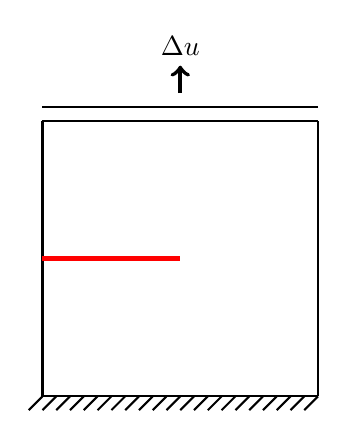
\begin{tikzpicture}[scale=0.7]
    \coordinate (K) at (0,0);
    % Square
    \draw[line width=0.75pt,black] (-2.5,-2.5) to (2.5,-2.5);
    \draw[line width=0.75pt,black] (2.5,-2.5) to (2.5,2.5);
    \draw[line width=0.75pt,black] (2.5,2.5) to (-2.5,2.5);
    \draw[line width=0.75pt,black] (-2.5,2.5) to (-2.5,-2.5);
    \draw[line width=1.5pt,red] (-2.5,0) to (0,0);
    % Top Boundary
    \draw[line width=0.75pt,black] (2.5,2.75) to (-2.5,2.75);
    \draw[->,line width=1.5pt,black] (0.0,3.0) to (0.0,3.5);
    \node[ ] at (0,3.85) {$\Delta\disp$};
    % Bottom Boundary
    \draw[line width=0.75pt,black] (-2.5,-2.5) to (-2.75,-2.75);
    \draw[line width=0.75pt,black] (-2.25,-2.5) to (-2.5,-2.75);
    \draw[line width=0.75pt,black] (-2.0,-2.5) to (-2.25,-2.75);
    \draw[line width=0.75pt,black] (-1.75,-2.5) to (-2.0,-2.75);
    \draw[line width=0.75pt,black] (-1.5,-2.5) to (-1.75,-2.75);
    \draw[line width=0.75pt,black] (-1.25,-2.5) to (-1.5,-2.75);
    \draw[line width=0.75pt,black] (-1.0,-2.5) to (-1.25,-2.75);
    \draw[line width=0.75pt,black] (-0.75,-2.5) to (-1.0,-2.75);
    \draw[line width=0.75pt,black] (-0.5,-2.5) to (-0.75,-2.75);
    \draw[line width=0.75pt,black] (-0.25,-2.5) to (-0.5,-2.75);
    \draw[line width=0.75pt,black] (0.0,-2.5) to (-0.25,-2.75);
    \draw[line width=0.75pt,black] (0.25,-2.5) to (0.0,-2.75);
    \draw[line width=0.75pt,black] (0.5,-2.5) to (0.25,-2.75);
    \draw[line width=0.75pt,black] (0.75,-2.5) to (0.5,-2.75);
    \draw[line width=0.75pt,black] (1.0,-2.5) to (0.75,-2.75);
    \draw[line width=0.75pt,black] (1.25,-2.5) to (1.0,-2.75);
    \draw[line width=0.75pt,black] (1.5,-2.5) to (1.25,-2.75);
    \draw[line width=0.75pt,black] (1.75,-2.5) to (1.5,-2.75);
    \draw[line width=0.75pt,black] (2.0,-2.5) to (1.75,-2.75);
    \draw[line width=0.75pt,black] (2.25,-2.5) to (2.0,-2.75);
    \draw[line width=0.75pt,black] (2.5,-2.5) to (2.25,-2.75);
    \end{tikzpicture}
\caption{SENT experiment}
\label{sec4:fig:tension}
\end{minipage}
\begin{minipage}[b]{0.45\linewidth}
\centering
\begin{tabular}{ll} \hline
  \textbf{Parameters} & \textbf{Value} \\ \hline
  Fracture Model & AT2 \\
  Energy Split & No Split \\
  $E_0$ & 210.0 [GPa] \\
  $\nu$ & 0.3 [-] \\
  $\gc$ & 2.7 [N/mm] \\
  $\l$ & 1.5e-2 [mm] \\
  $\eta$ & $\beta \gc/\l$ \\ \hline
  \end{tabular}
\captionof{table}{Model parameters}
\label{sec4:table:miehe_tension}
\end{minipage}
\end{figure}

Figure \ref{sec4:fig:miehe_tension_lodi} present the load-displacement curves, corresponding to the brittle AT2 model. They are compared with the load-displacement curves from the literature \cite{Miehe2010,Ambati2015,KRISTENSEN2020104093}. While $\beta = 100, 200$ yield curves similar to those obtained by \cite{Ambati2015}, $\beta = 10$ results in under-estimation of the peak load. The latter observation is due to the insufficient regularization of the phase-field. This is evident from Figure \ref{sec4:fig:sentProfile10}, where the phase-field $\pf$ and the micromorphic variable $\mpf$ is plotted for a section, $x = 0.75$ [mm] of the specimen. Therein, a localized behaviour is observed for $\pf \geq 0.6$. Upon increasing $\beta$ to $100$ and $200$, the $\pf$ and $\mpf$ curves are similar, i.e., $\pf \approx \mpf$, which is an indication of sufficient regularization. When $\pf \approx \mpf$, the micromorphic phase-field fracture model is similar to the conventional phase-field fracture model. This explains the similar load-displacement curves for $\beta = 100,200$ and those obtained with conventional phase-field fracture model in the literature \cite{Miehe2010,Ambati2015,KRISTENSEN2020104093}. Moreover, the phase-field fracture topology in the final step of the simulation in Figure \ref{sec4:fig:pf_sen_tension_failure} is also similar to those in the literature \cite{Miehe2010,Ambati2015,KRISTENSEN2020104093}.

\begin{figure}[!ht]
  \begin{subfigure}[t]{0.45\textwidth}
  \centering
  \begin{tikzpicture}[thick,scale=0.95, every node/.style={scale=1.0}]
    \begin{axis}[width=9.5cm,height=5.75cm,legend style={draw=none,at={(0.5,1.375)},anchor=north,legend cell align=left}, legend columns = 2,
      transpose legend, ylabel={Load\:[kN]},xlabel={Displacement\:[mm]}, xmin=0, ymin=0, xmax=0.0065, ymax=0.8, yticklabel style={/pgf/number format/.cd,fixed,precision=2},
                 every axis plot/.append style={thick}]
    \pgfplotstableread{./Data/SENT/NotchTension_Miehe.txt}\Adata;
    \pgfplotstableread{./Data/SENT/martinez.txt}\Bdata;
    \pgfplotstableread{./Data/SENT/NotchTension_Ambati.txt}\Cdata;
    \pgfplotstableread{./Data/SENT/problem_lodi_10.dat}\Ddata;
    \pgfplotstableread{./Data/SENT/problem_lodi_100.dat}\Edata;
    \pgfplotstableread{./Data/SENT/problem_lodi_200.dat}\Fdata;
    \addplot [ 
           color=black, 
%           only marks, 
           mark=*, 
           mark size=0.05pt, 
         ]
         table
         [
           x expr=\thisrowno{0}, 
           y expr=\thisrowno{1}
         ] {\Adata};
         \addlegendentry{Miehe [19]}
    \addplot [ 
           color=red, 
%           only marks, 
           mark=*, 
           mark size=0.05pt, 
         ]
         table
         [
           x expr=\thisrowno{0}, 
           y expr=\thisrowno{1}/1e3
         ] {\Bdata};
         \addlegendentry{Kristensen [62]}
    \addplot [ 
           color=blue, 
%           only marks, 
           mark=*, 
           mark size=0.25pt, 
         ]
         table
         [
           x expr=\thisrowno{0}, 
           y expr=\thisrowno{1}
         ] {\Cdata};
         \addlegendentry{Ambati [45]} 
    \addplot [ 
           color=green, 
%           only marks, 
           mark=*, 
           mark size=0.05pt, 
         ]
         table
         [
           x expr=\thisrowno{0}, 
           y expr=\thisrowno{1}/1e3
         ] {\Ddata};
         \addlegendentry{10} 
    \addplot [ 
           color=cyan, 
%           only marks, 
           mark=*, 
           mark size=0.05pt, 
         ]
         table
         [
           x expr=\thisrowno{0}, 
           y expr=\thisrowno{1}/1e3
         ] {\Edata};
         \addlegendentry{100}
    \addplot [ 
           color=magenta, 
%           only marks, 
           mark=*, 
           mark size=0.05pt, 
         ]
         table
         [
           x expr=\thisrowno{0}, 
           y expr=\thisrowno{1}/1e3
         ] {\Fdata};
         \addlegendentry{200}
    \end{axis}
    \end{tikzpicture}
    \caption{ }
    \label{sec4:fig:miehe_tension_lodi}
  \end{subfigure}
  \hfill
  %
  \begin{subfigure}[t]{0.45\textwidth}
  \centering
    \begin{tikzpicture}
    \node[inner sep=0pt] () at (0,0)
    {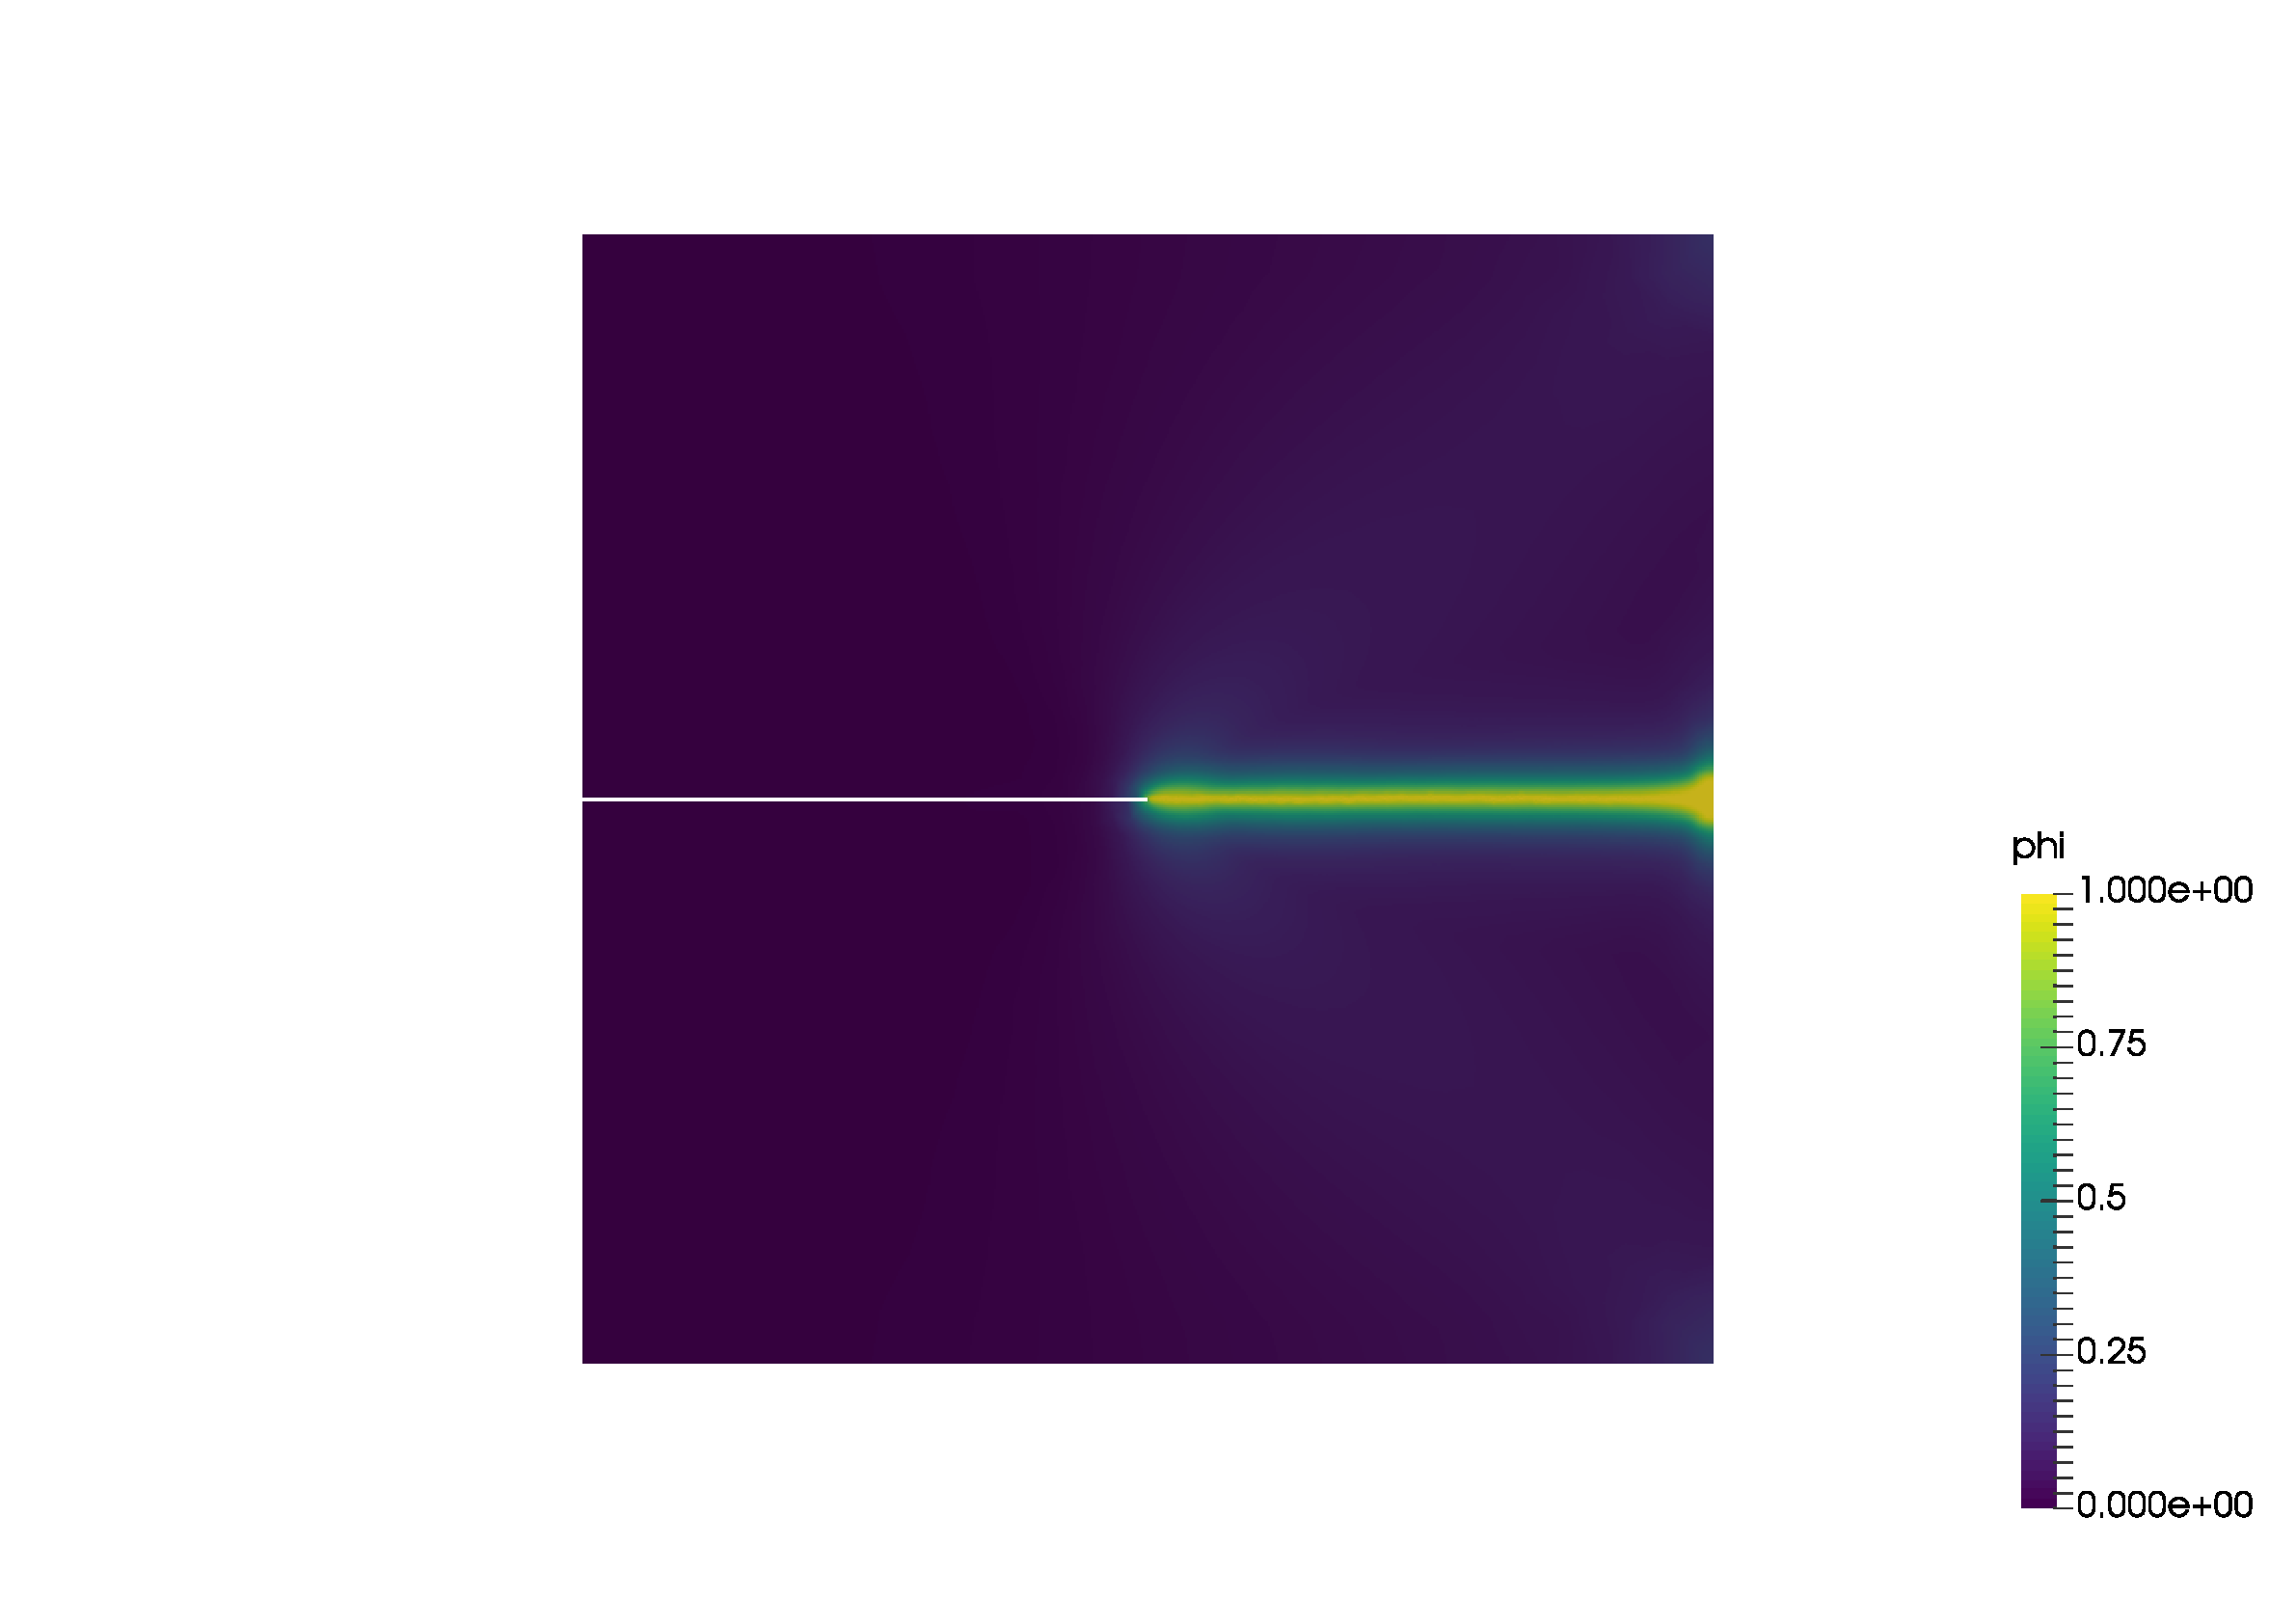
\includegraphics[width=6.0cm,trim=7cm 1cm 7cm 1cm, clip]{Images/SingleEdgeNotchedTension/sent_pf.pdf}};
    \node[inner sep=0pt] () at (-1.15,-3.05)
    {\begin{axis}[
    hide axis,
    scale only axis,
    height=0pt,
    width=0pt,
    colormap/viridis,
    colorbar horizontal,
    point meta min=0,
    point meta max=1,
    colorbar style={
        width=4.75cm,
        xtick={0,0.5,1.0},
        xticklabel style = {yshift=-0.075cm}
    }]
    \addplot [draw=none] coordinates {(0,0)};
    \end{axis}};
    \node[inner sep=0pt] () at (0,-3.75) {$\pf$};
    \end{tikzpicture}
    \caption{ }
    \label{sec4:fig:pf_sen_tension_failure}
  \end{subfigure}
  \caption{Figure (a) presents the load-displacement curves for the single edge notched specimen under tension. Here, $\beta$ is varied as \{10,100,200\}. Figure (b) shows the distribution of the phase-field variable at the final step of the analysis.}
\end{figure}

% Profiles

\begin{figure}[!ht]
  \begin{subfigure}[t]{0.3\textwidth}
  \centering
  \begin{tikzpicture}[thick,scale=0.95, every node/.style={scale=1.0}]
    \begin{axis}[width=4.75cm,height=5.75cm,legend style={draw=none,at={(0.5,1.375)},anchor=north,legend cell align=left}, legend columns = 2,
      transpose legend, ylabel={Value\:[-]},xlabel={Height\:[mm]}, xmin=0, ymin=0, xmax=1., ymax=1.0, yticklabel style={/pgf/number format/.cd,fixed,precision=2},
                 every axis plot/.append style={thick}]
    \pgfplotstableread[col sep = comma]{./Data/SENT/profile10.txt}\Adata;
    \addplot [ 
           color=black, 
%           only marks, 
           mark=*, 
           mark size=0.05pt, 
         ]
         table
         [
           x expr=\thisrowno{0}, 
           y expr=\thisrowno{1}
         ] {\Adata};
         \addlegendentry{$\pf$}
    \addplot [ 
           color=red, 
%           only marks, 
           mark=*, 
           mark size=0.05pt, 
         ]
         table
         [
           x expr=\thisrowno{0}, 
           y expr=\thisrowno{2}
         ] {\Adata};
         \addlegendentry{\mpf}
    \end{axis}
    \end{tikzpicture}
    \caption{$\beta = 10$}
    \label{sec4:fig:sentProfile10}
  \end{subfigure}
  \hfill
  %
  \begin{subfigure}[t]{0.3\textwidth}
  \centering
  \begin{tikzpicture}[thick,scale=0.95, every node/.style={scale=1.0}]
    \begin{axis}[width=4.75cm,height=5.75cm,legend style={draw=none,at={(0.5,1.375)},anchor=north,legend cell align=left}, legend columns = 2,
      transpose legend, xlabel={Height\:[mm]}, xmin=0, ymin=0, xmax=1., ymax=1.0, yticklabel style={/pgf/number format/.cd,fixed,precision=2},
                 every axis plot/.append style={thick}]
    \pgfplotstableread[col sep = comma]{./Data/SENT/profile100.txt}\Adata;
    \addplot [ 
           color=black, 
%           only marks, 
           mark=*, 
           mark size=0.05pt, 
         ]
         table
         [
           x expr=\thisrowno{0}, 
           y expr=\thisrowno{1}
         ] {\Adata};
         \addlegendentry{$\pf$}
    \addplot [ 
           color=red, 
%           only marks, 
           mark=*, 
           mark size=0.05pt, 
         ]
         table
         [
           x expr=\thisrowno{0}, 
           y expr=\thisrowno{2}
         ] {\Adata};
         \addlegendentry{\mpf}
    \end{axis}
    \end{tikzpicture}
    \caption{$\beta = 100$}
    \label{sec4:fig:sentProfile100}
  \end{subfigure}
  \hfill
  \begin{subfigure}[t]{0.3\textwidth}
  \centering
  \begin{tikzpicture}[thick,scale=0.95, every node/.style={scale=1.0}]
    \begin{axis}[width=4.75cm,height=5.75cm,legend style={draw=none,at={(0.5,1.375)},anchor=north,legend cell align=left}, legend columns = 2,
      transpose legend, xlabel={Height\:[mm]}, xmin=0, ymin=0, xmax=1., ymax=1.0, yticklabel style={/pgf/number format/.cd,fixed,precision=2},
                 every axis plot/.append style={thick}]
    \pgfplotstableread[col sep = comma]{./Data/SENT/profile200.txt}\Adata;
    \addplot [ 
           color=black, 
%           only marks, 
           mark=*, 
           mark size=0.05pt, 
         ]
         table
         [
           x expr=\thisrowno{0}, 
           y expr=\thisrowno{1}
         ] {\Adata};
         \addlegendentry{$\pf$}
    \addplot [ 
           color=red, 
%           only marks, 
           mark=*, 
           mark size=0.05pt, 
         ]
         table
         [
           x expr=\thisrowno{0}, 
           y expr=\thisrowno{2}
         ] {\Adata};
         \addlegendentry{\mpf}
    \end{axis}
    \end{tikzpicture}
    \caption{$\beta = 200$}
    \label{sec4:fig:sentProfile200}
  \end{subfigure}
  \caption{Figures present the phase-field ($\pf$) and the micromorphic variable ($\mpf$) for different $\beta$ values at $x=0.75$ [mm], along the height of the SENT specimen.}
\end{figure}

\subsection{Single Edge Notched specimen under Shear (SENS)}\label{sec4:SENshear}

The single edge notched specimen in the previous section is loaded horizontally along the top edge as shown in Figure \ref{sec4:fig:miehe_shear} for a shear test. Following the recommendations in \cite{Ambati2015}, the geometry is discretised with four-noded quad elements with four integration points. The relevant model parameters are presented in Table \ref{sec4:table:miehe_shear}, where a spectral decomposition based energy split is adopted to capture the tension-compression asymmetric response. A quasi-static loading is applied to the top boundary in the form of prescribed displacement increment $\Delta\disp = 1e-4$[mm] for the first $85$ steps, following which it is changed to $1e-6$[mm]. Furthermore, the bottom boundary remains fixed, and roller supports are implemented in left and right edges restricting the vertical displacement.

\begin{figure}[ht]
\begin{minipage}[b]{0.45\linewidth}
\centering
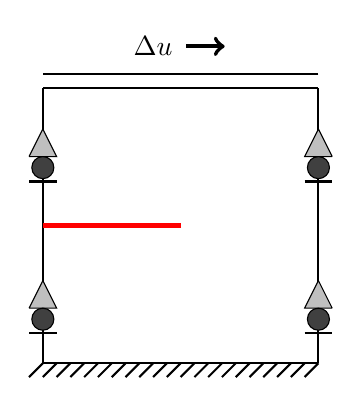
\begin{tikzpicture}[scale=0.7]
    \coordinate (K) at (0,0);
    % Square
    \draw[line width=0.75pt,black] (-2.5,-2.5) to (2.5,-2.5);
    \draw[line width=0.75pt,black] (2.5,-2.5) to (2.5,2.5);
    \draw[line width=0.75pt,black] (2.5,2.5) to (-2.5,2.5);
    \draw[line width=0.75pt,black] (-2.5,2.5) to (-2.5,-2.5);
    \draw[line width=1.5pt,red] (-2.5,0) to (0,0);
    % Top Boundary
    \draw[line width=0.75pt,black] (2.5,2.75) to (-2.5,2.75);
    \draw[->,line width=1.5pt,black] (0.1,3.25) to (0.8,3.25);
    \node[ ] at (-0.5,3.25) {$\Delta\disp$};
    %\node[ ] at (0,3.85) {$\disp_y=0$};
    % Bottom Boundary
    \draw[line width=0.75pt,black] (-2.5,-2.5) to (-2.75,-2.75);
    \draw[line width=0.75pt,black] (-2.25,-2.5) to (-2.5,-2.75);
    \draw[line width=0.75pt,black] (-2.0,-2.5) to (-2.25,-2.75);
    \draw[line width=0.75pt,black] (-1.75,-2.5) to (-2.0,-2.75);
    \draw[line width=0.75pt,black] (-1.5,-2.5) to (-1.75,-2.75);
    \draw[line width=0.75pt,black] (-1.25,-2.5) to (-1.5,-2.75);
    \draw[line width=0.75pt,black] (-1.0,-2.5) to (-1.25,-2.75);
    \draw[line width=0.75pt,black] (-0.75,-2.5) to (-1.0,-2.75);
    \draw[line width=0.75pt,black] (-0.5,-2.5) to (-0.75,-2.75);
    \draw[line width=0.75pt,black] (-0.25,-2.5) to (-0.5,-2.75);
    \draw[line width=0.75pt,black] (0.0,-2.5) to (-0.25,-2.75);
    \draw[line width=0.75pt,black] (0.25,-2.5) to (0.0,-2.75);
    \draw[line width=0.75pt,black] (0.5,-2.5) to (0.25,-2.75);
    \draw[line width=0.75pt,black] (0.75,-2.5) to (0.5,-2.75);
    \draw[line width=0.75pt,black] (1.0,-2.5) to (0.75,-2.75);
    \draw[line width=0.75pt,black] (1.25,-2.5) to (1.0,-2.75);
    \draw[line width=0.75pt,black] (1.5,-2.5) to (1.25,-2.75);
    \draw[line width=0.75pt,black] (1.75,-2.5) to (1.5,-2.75);
    \draw[line width=0.75pt,black] (2.0,-2.5) to (1.75,-2.75);
    \draw[line width=0.75pt,black] (2.25,-2.5) to (2.0,-2.75);
    \draw[line width=0.75pt,black] (2.5,-2.5) to (2.25,-2.75);
    % Left edge 1
    \draw[fill=gray!50] (-2.75,1.25) -- (-2.25,1.25) -- (-2.5,1.75)-- (-2.75,1.25);
    \draw[fill=black!75] (-2.5,1.05) circle (0.2);
    \draw[line width=1pt,black] (-2.25,0.8) to (-2.75,0.8);
    % Left edge 2
    \draw[fill=gray!50] (-2.75,-1.5) -- (-2.25,-1.5) -- (-2.5,-1.)-- (-2.75,-1.5);
    \draw[fill=black!75] (-2.5,-1.7) circle (0.2);
    \draw[line width=1pt,black] (-2.25,-1.95) to (-2.75,-1.95);
    % Right edge 1
    \draw[fill=gray!50] (2.75,1.25) -- (2.25,1.25) -- (2.5,1.75)-- (2.75,1.25);
    \draw[fill=black!75] (2.5,1.05) circle (0.2);
    \draw[line width=1pt,black] (2.25,0.8) to (2.75,0.8);
    % Right edge 2
    \draw[fill=gray!50] (2.75,-1.5) -- (2.25,-1.5) -- (2.5,-1.)-- (2.75,-1.5);
    \draw[fill=black!75] (2.5,-1.7) circle (0.2);
    \draw[line width=1pt,black] (2.25,-1.95) to (2.75,-1.95);
    \end{tikzpicture}
\caption{SENS experiment}
\label{sec4:fig:miehe_shear}
\end{minipage}
\begin{minipage}[b]{0.45\linewidth}
\centering
\begin{tabular}{ll} \hline
  \textbf{Parameters} & \textbf{Value} \\ \hline
  Fracture Model & AT2 \\
  Energy Split & Spectral \\
  $E_0$ & 210.0 [GPa] \\
  $\nu$ & 0.3 [-] \\
  $\gc$ & 2.7 [N/mm] \\
  $\l$ & 1.5e-2 [mm] \\
  $\eta$ & $\beta \gc/\l$ \\ \hline
  \end{tabular}
\captionof{table}{Model parameters}
\label{sec4:table:miehe_shear}
\end{minipage}
\end{figure}

Figure \ref{sec4:fig:miehe_shear_lodi} shows the load displacement curves obtained using $\beta = 10, 100, 200$, and from \cite{Miehe2010}. The curves from \cite{Ambati2015,KRISTENSEN2020102446} are excluded since the former adopts a variationally inconsistent hybrid formulation, and the latter used a different set of boundary conditions. While $\beta = 100, 200$ yield curves similar to those obtained by \cite{Miehe2010}, $\beta = 10$ results in under-estimation of the peak load. The latter observation is due to the insufficient regularization of the phase-field. The effect of the insufficient regularization has been explained in the previous sub-section. Moreover, the phase-field topology at the final step of the analysis is presented in Figure \ref{sec4:fig:pf_sen_shear_failure}), where the fracture path is similar to that presented in \cite{Miehe2010}. 

\begin{figure}[!ht]
  \begin{subfigure}[t]{0.45\textwidth}
  \centering
  \begin{tikzpicture}[thick,scale=0.95, every node/.style={scale=1.0}]
    \begin{axis}[width=9.5cm,height=5.75cm,legend style={draw=none,at={(0.5,1.375)},anchor=north,legend cell align=left}, legend columns = 3,
       ylabel={Load\:[kN]},xlabel={Displacement\:[mm]}, xmin=0, ymin=0, xmax=0.014, ymax=0.55, yticklabel style={/pgf/number format/.cd,fixed,precision=2},
                 every axis plot/.append style={thick}]
    \pgfplotstableread{./Data/SENS/problem_lodi100.dat}\Adata;
    \pgfplotstableread{./Data/SENS/problem_lodi200.dat}\Cdata;
    \pgfplotstableread{./Data/SENS/problem_lodi10.dat}\Ddata;
    \pgfplotstableread{./Data/SENS/NotchShear_Miehe.txt}\Bdata;
    \addplot [ 
           color=black, 
%           only marks, 
           mark=*, 
           mark size=0.05pt, 
         ]
         table
         [
           x expr=\thisrowno{0}, 
           y expr=\thisrowno{1}
         ] {\Bdata};
         \addlegendentry{Miehe [19]}     
    \addplot [ 
           color=green, 
%           only marks, 
           mark=*, 
           mark size=0.05pt, 
         ]
         table
         [
           x expr=\thisrowno{0}, 
           y expr=\thisrowno{1}/1e3
         ] {\Ddata};
         \addlegendentry{10}
    \addplot [ 
           color=cyan, 
%           only marks, 
           mark=*, 
           mark size=0.05pt, 
         ]
         table
         [
           x expr=\thisrowno{0}, 
           y expr=\thisrowno{1}/1e3
         ] {\Adata};
         \addlegendentry{100}
    \addplot [ 
           color=magenta, 
%           only marks, 
           mark=*, 
           mark size=0.05pt, 
         ]
         table
         [
           x expr=\thisrowno{0}, 
           y expr=\thisrowno{1}/1e3
         ] {\Cdata};
         \addlegendentry{200}
    \end{axis}
    \end{tikzpicture}
    \caption{ }
    \label{sec4:fig:miehe_shear_lodi}
  \end{subfigure}
  \hfill
  %
  \begin{subfigure}[t]{0.45\textwidth}
  \centering
    \begin{tikzpicture}
    \node[inner sep=0pt] () at (0,0)
    {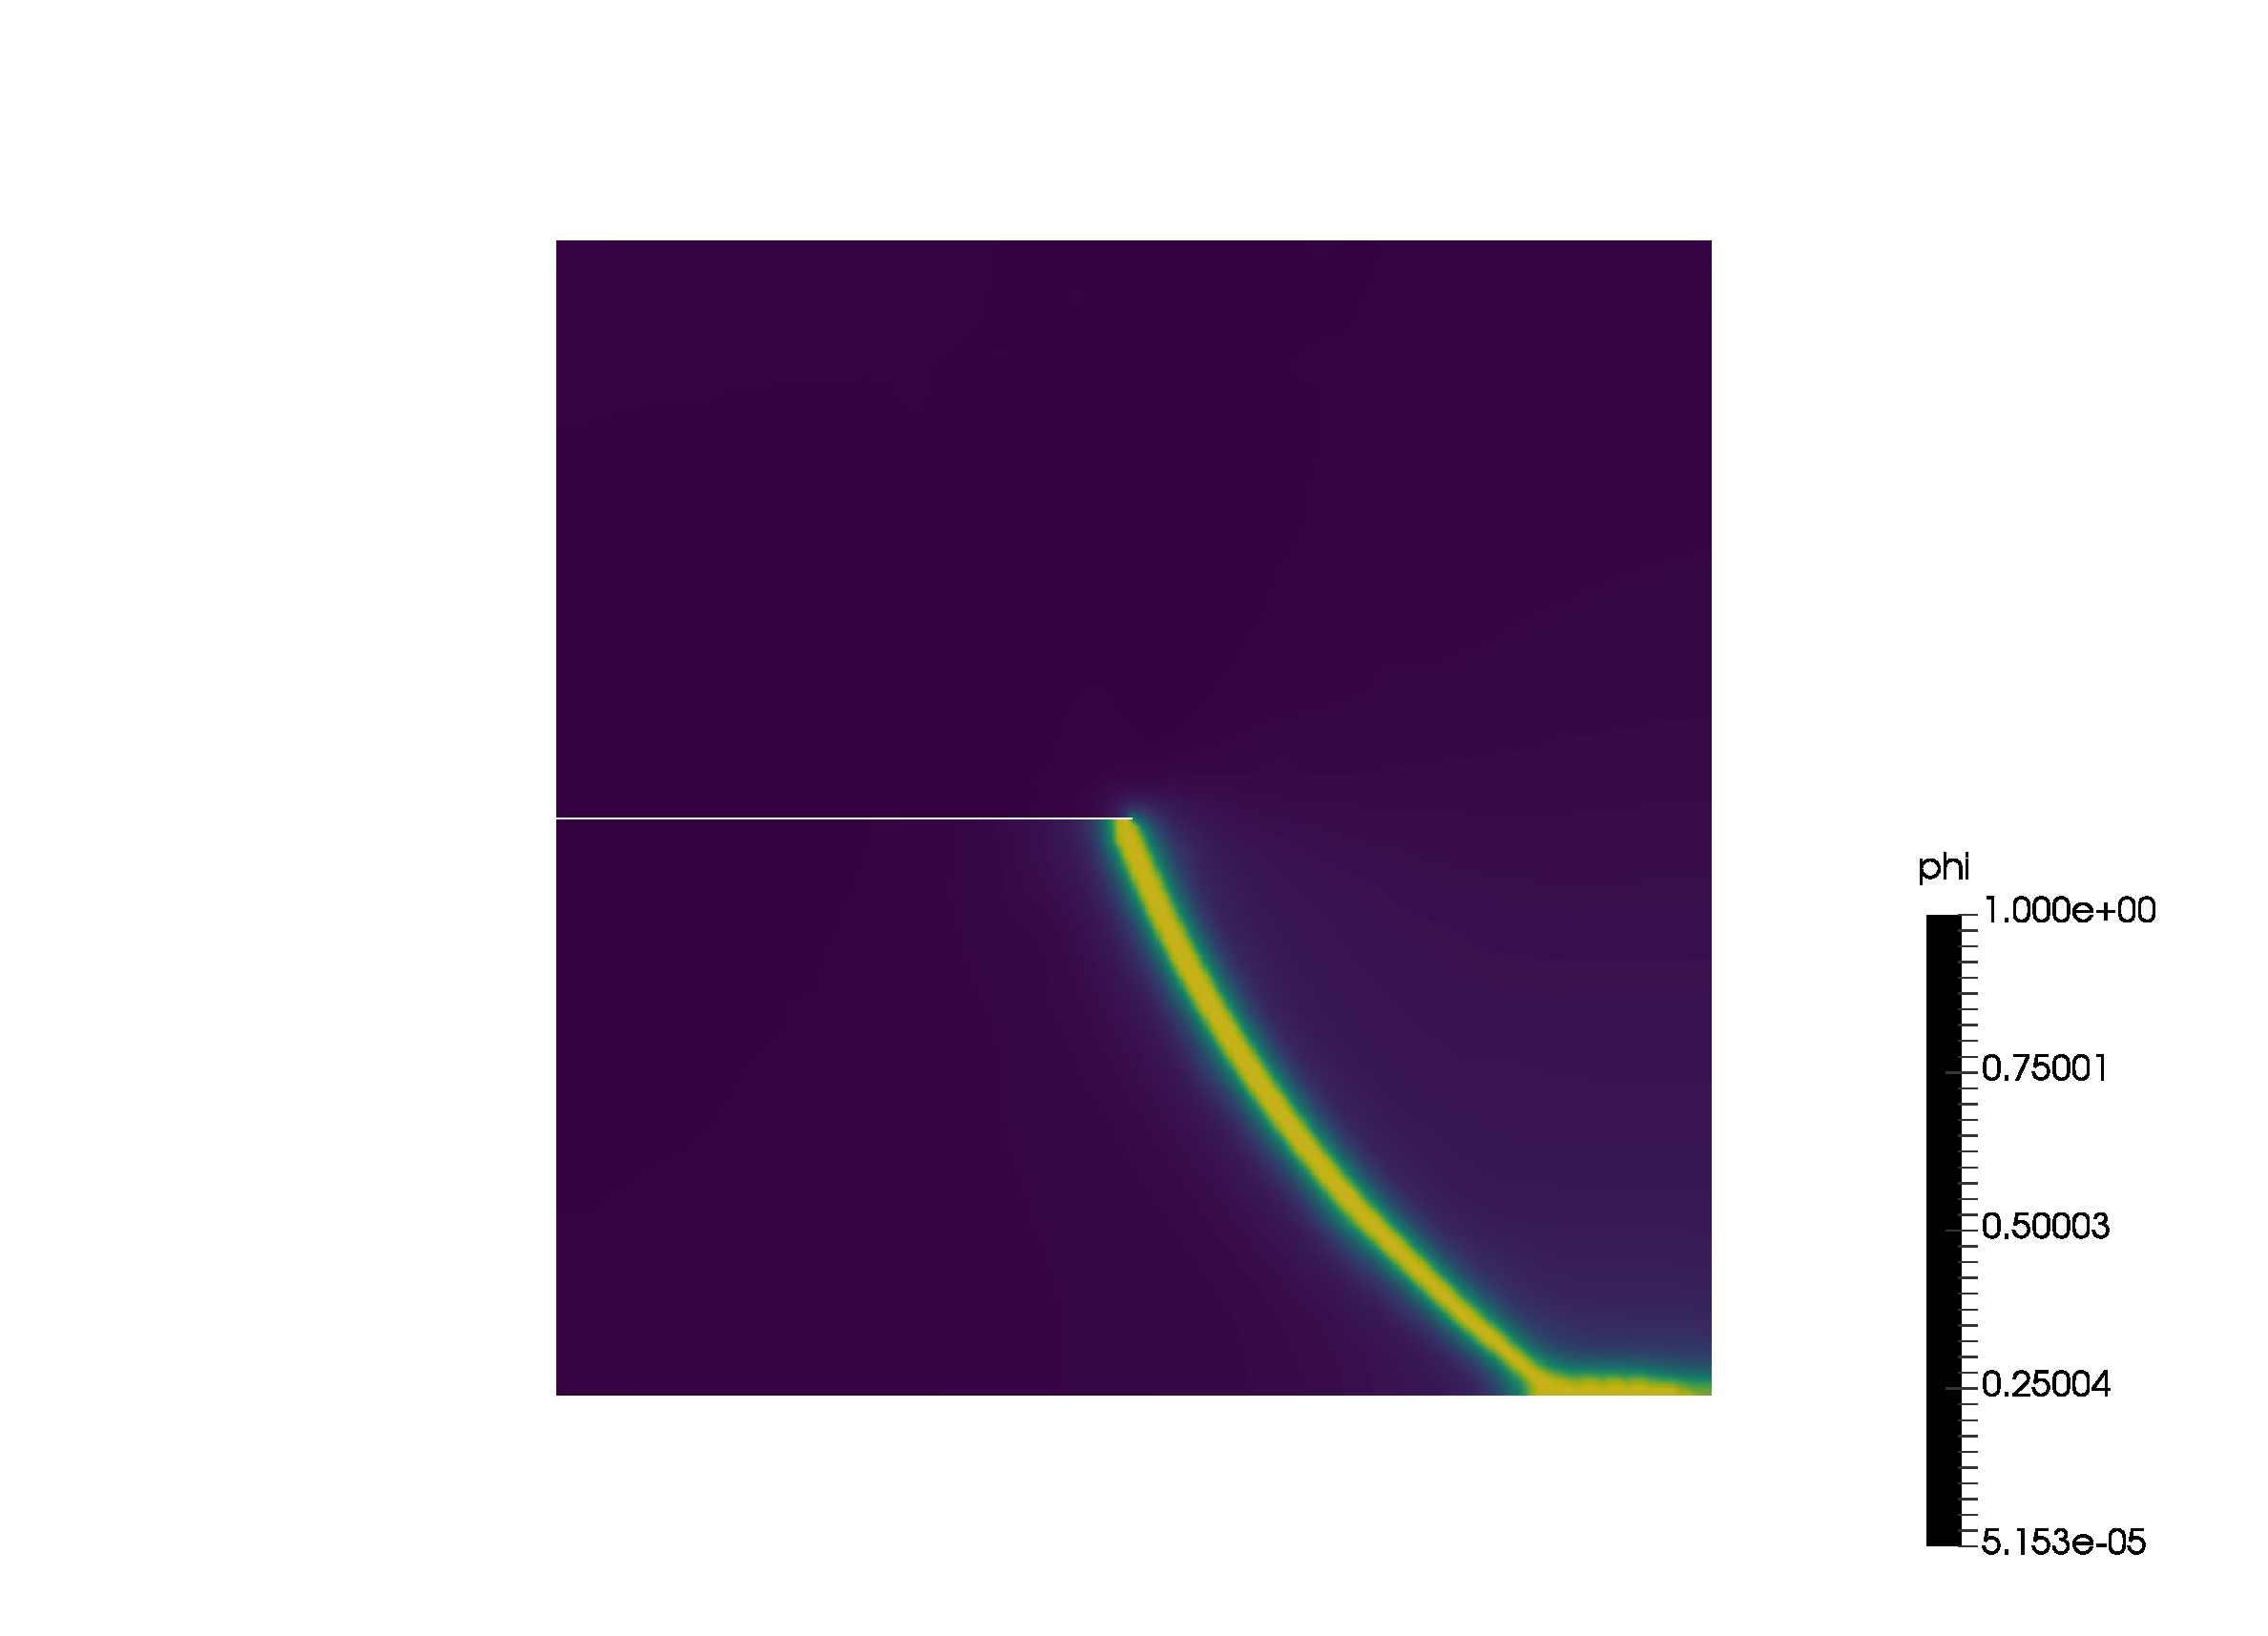
\includegraphics[width=6.0cm,trim=7cm 1cm 7cm 1cm, clip]{Images/SingleEdgeNotchedShear/sens_pf1.pdf}};
    \node[inner sep=0pt] () at (-1.15,-3.05)
    {\begin{axis}[
    hide axis,
    scale only axis,
    height=0pt,
    width=0pt,
    colormap/viridis,
    colorbar horizontal,
    point meta min=0,
    point meta max=1,
    colorbar style={
        width=4.75cm,
        xtick={0,0.5,1.0},
        xticklabel style = {yshift=-0.075cm}
    }]
    \addplot [draw=none] coordinates {(0,0)};
    \end{axis}};
    \node[inner sep=0pt] () at (0,-3.75) {$\pf$};
    \end{tikzpicture}
    \caption{ }
    \label{sec4:fig:pf_sen_shear_failure}
  \end{subfigure}
  \caption{Figure (a) presents the load-displacement curves for the single edge notched specimen under shear. Here, $\beta$ is varied as \{10,100,200\}. Figure (b) shows the distribution of the phase-field variable at the final step of the analysis.}
\end{figure}

\subsection{Winkler L-panel}\label{sec4:Lpanel}

The concrete L-shaped panel studied by \cite{winkler2001traglastuntersuchungen,unger2007modelling} is considered in this sub-section. Figure \ref{sec4:fig:Lpanel} shows the geometry as well as the loading conditions. The longer edges of the panel are 500 [mm] and the smaller edges are 250 [mm]. The loading is applied on the edge marked in blue, 30 [mm] in length, and is in the form of displacement increments of $\Delta\disp = 1e-3$ [mm]. The model parameters are presented in Table \ref{sec4:table:Lpanel_params}. The reader is referred to Section \ref{sec2:energyFunc} for a detailed explanation of these parameters.

\begin{figure}[ht]
\begin{minipage}[b]{0.45\linewidth}
\centering
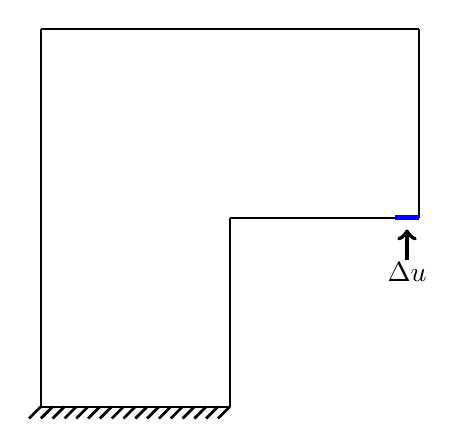
\begin{tikzpicture}[scale=0.6]
    \coordinate (K) at (0,0);
    % Square
    \draw[line width=0.75pt,black] (-4,-4) to (0,-4);
    \draw[line width=0.75pt,black] (0,-4) to (0,0);
    \draw[line width=0.75pt,black] (0,0) to (4,0);
    \draw[line width=0.75pt,black] (4,0)  to (4,4);
    \draw[line width=0.75pt,black] (4,4) to (-4,4);
    \draw[line width=0.75pt,black] (-4,4) to (-4,-4);
    % Loading
    \draw[line width=2.0pt,blue] (3.5,0) to (4,0);
    \draw[->,line width=1.5pt,black] (3.75,-0.9) to (3.75,-0.25);
    \node[ ] at (3.75,-1.15) {$\Delta\disp$};
    % Left edge
    %\draw[fill=black!75] (-2.5,1.05) circle (0.2);
    \draw[line width=1pt,black] (0,-4) to (-0.25,-4.25);
    \draw[line width=1pt,black] (-0.25,-4.) to (-0.5,-4.25);
    \draw[line width=1pt,black] (-0.5,-4.) to (-0.75,-4.25);
    \draw[line width=1pt,black] (-0.75,-4.) to (-1,-4.25);
    \draw[line width=1pt,black] (-1,-4.) to (-1.25,-4.25);
    \draw[line width=1pt,black] (-1.25,-4.) to (-1.5,-4.25);
    \draw[line width=1pt,black] (-1.5,-4.) to (-1.75,-4.25);
    \draw[line width=1pt,black] (-1.75,-4.) to (-2.,-4.25);
    \draw[line width=1pt,black] (-2.,-4.) to (-2.25,-4.25);
    \draw[line width=1pt,black] (-2.25,-4.) to (-2.5,-4.25);
    \draw[line width=1pt,black] (-2.5,-4.) to (-2.75,-4.25);
    \draw[line width=1pt,black] (-2.75,-4.) to (-3.,-4.25);
    \draw[line width=1pt,black] (-3.,-4.) to (-3.25,-4.25);
    \draw[line width=1pt,black] (-3.25,-4.) to (-3.5,-4.25);
    \draw[line width=1pt,black] (-3.5,-4.) to (-3.75,-4.25);
    \draw[line width=1pt,black] (-3.75,-4.) to (-4.,-4.25);
    \draw[line width=1pt,black] (-4.,-4.) to (-4.25,-4.25);
    \end{tikzpicture}
\caption{Winkler L-panel}
\label{sec4:fig:Lpanel}
\end{minipage}
\hspace{0.5cm}
\begin{minipage}[b]{0.45\linewidth}
\centering
\begin{tabular}{ll} \hline
  \textbf{Parameters}  & \textbf{Value} \\ \hline
  Fracture Model & Quasi-Brittle \\
  Energy Split & Spectral \\
  Softening & Cornellisen et. al. \cite{cornelissen1986experimental} \\
  $E_0$  & 2.0e4 [MPa] \\
  $\nu$  & 0.18 [-] \\
  $f_t$  & 2.5 [MPa] \\
  $\gc$  & 0.130 [N/mm] \\
  $\l$  & 10 [mm] \\
  $\eta$ & $\beta \gc/\l$ \\ \hline
  \end{tabular}
\captionof{table}{Parameters for L-shaped panel test \cite{unger2007modelling}}
\label{sec4:table:Lpanel_params}
\end{minipage}
\end{figure}

\begin{figure}[!ht]
\centering
  \begin{subfigure}[t]{0.45\textwidth}
  \centering
    \begin{tikzpicture}[thick,scale=0.95, every node/.style={scale=1.175}]
    \begin{axis}[legend style={draw=none}, legend columns = 3,
      transpose legend, ylabel={Load\:[kN]},xlabel={Displacement\:[mm]}, xmin=0, ymin=0, xmax=1.0, ymax=8.0, yticklabel style={
        /pgf/number format/fixed,
        /pgf/number format/precision=5
        },
        scaled y ticks=false,
        xticklabel style={
        /pgf/number format/fixed,
        /pgf/number format/precision=5
        },
        scaled x ticks=false,
        every axis plot/.append style={thick}]
    \pgfplotstableread{./Data/WinklerL/problem_lodi200m.dat}\Edata;
    \pgfplotstableread{./Data/WinklerL/problem_lodi100m.dat}\Cdata;
    \pgfplotstableread[col sep = comma]{./Data/WinklerL/LPanelUpperLodi.txt}\Bdata;
    \pgfplotstableread[col sep = comma]{./Data/WinklerL/LPanelLowerLodi.txt}\Adata;
    \addplot [ name path = A,
           color=blue!20, 
%           only marks, 
           mark=*, 
           mark size=0.01pt,
           forget plot
         ]
         table
         [
           x expr=\thisrowno{0}, 
           y expr=\thisrowno{1}
         ] {\Adata};
    \addplot [ name path = B,
           color=blue!20, 
%           only marks, 
           mark=*, 
           mark size=0.01pt, 
           forget plot
         ]
         table
         [
           x expr=\thisrowno{0}, 
           y expr=\thisrowno{1}
         ] {\Bdata};
    % Fill area between paths
    \addplot [blue!20, forget plot] fill between [of = A and B];     
    \addplot [ 
           color=cyan, 
%           only marks, 
           mark=*, 
           mark size=0.05pt, 
         ]
         table
         [
           x expr=\thisrowno{0}, 
           y expr=\thisrowno{1}/10
         ] {\Cdata};
         \addlegendentry{100}
    \addplot [ 
           color=magenta, 
%           only marks, 
           mark=*, 
           mark size=0.05pt, 
         ]
         table
         [
           x expr=\thisrowno{0}, 
           y expr=\thisrowno{1}/10
         ] {\Edata};
         \addlegendentry{200}     
    \end{axis}
    \end{tikzpicture}
    \caption{Load-displacement plot}
    \label{sec4:fig:LPanel_lodi}
  \end{subfigure}
  \hspace{5mm}
  %
  \begin{subfigure}[t]{0.45\textwidth}
  \centering
    \begin{tikzpicture}
    \node[inner sep=0pt] () at (0,1.5)
    {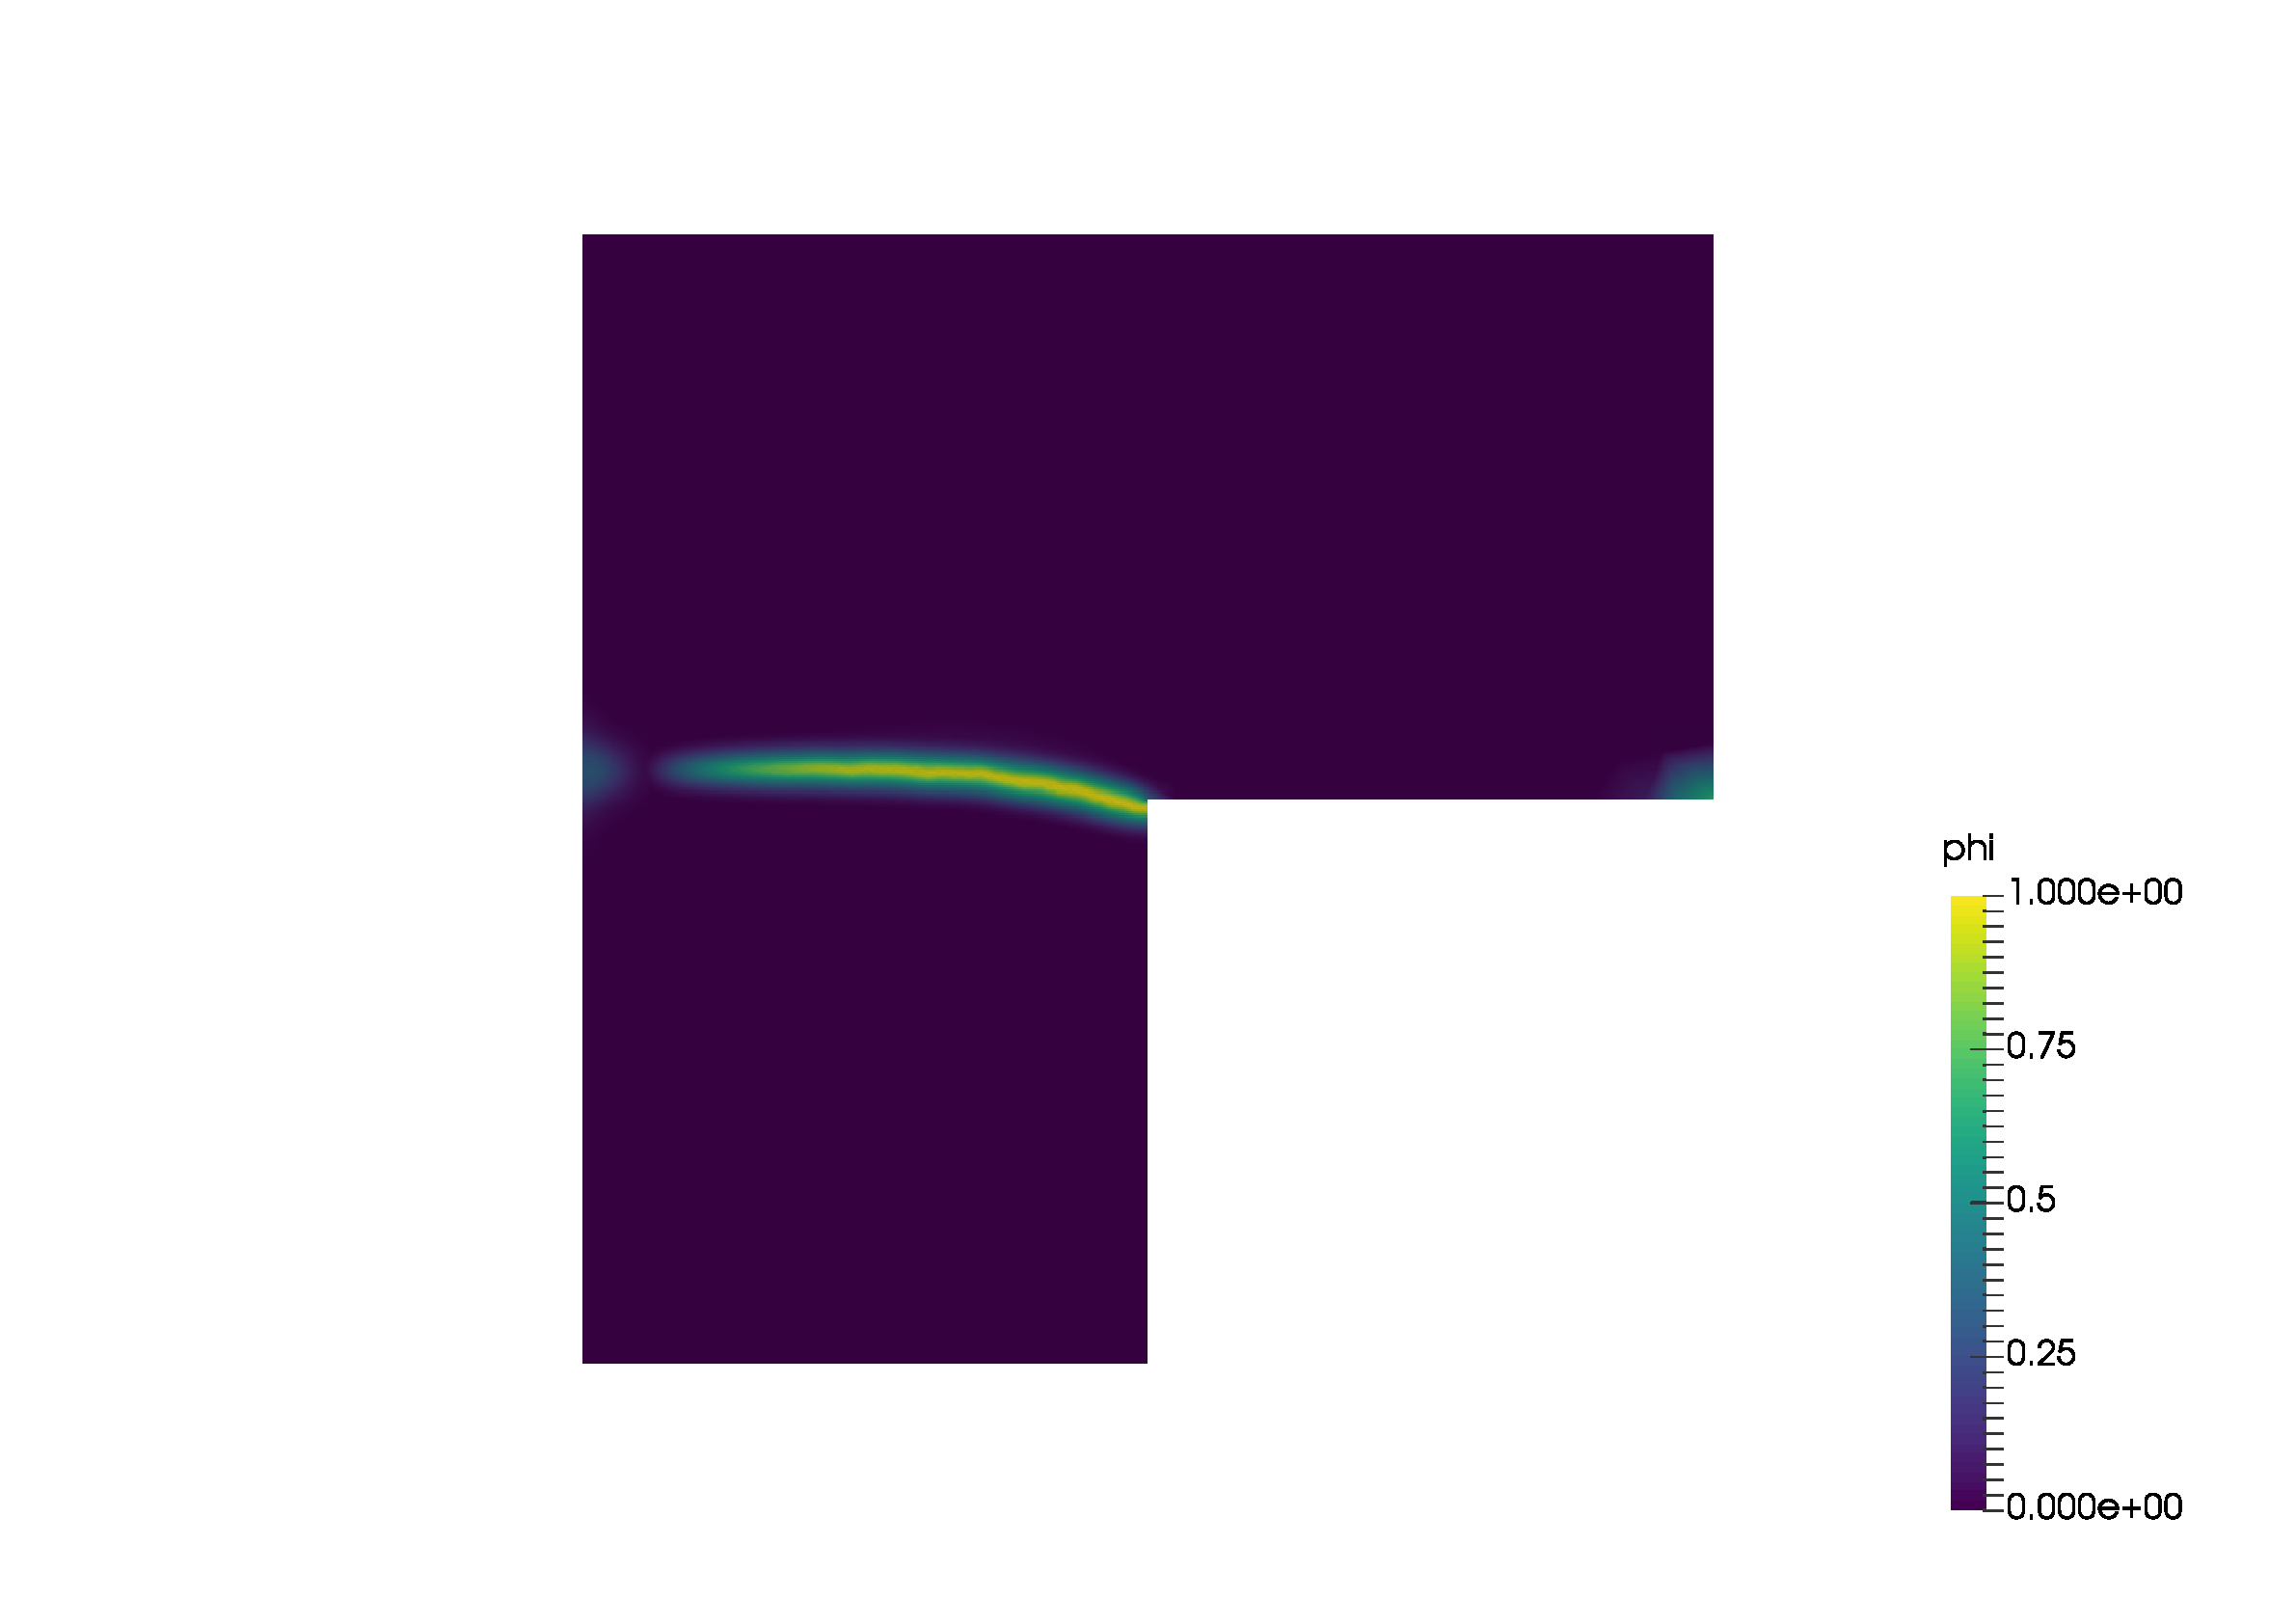
\includegraphics[width=6.0cm,trim=7cm 1cm 7cm 1cm, clip]{Images/WinklerL/winkler_pf.pdf}};
    \node[inner sep=0pt] () at (-1.2,-1.75)
    {\begin{axis}[
    hide axis,
    scale only axis,
    height=0pt,
    width=0pt,
    colormap/viridis,
    colorbar horizontal,
    point meta min=0,
    point meta max=1,
    colorbar style={
        width=4.75cm,
        xtick={0,0.5,1.0},
        xticklabel style = {yshift=-0.075cm}
    }]
    \addplot [draw=none] coordinates {(0,0)};
    \end{axis}};
    \node[inner sep=0pt] () at (0,-2.45) {$\pf$};
    \end{tikzpicture}
    \caption{ }
    \label{sec4:fig:pf_LPanel_failure}
  \end{subfigure}
  \caption{Figure (a) presents the load-displacement curves for the concrete Winkler L-panel test, for $\beta = 100, 200$. The experimental range is represented by the shaded area. Figure (b) shows the distribution of the phase-field variable at the final step of the analysis.}
  \label{sec4:fig:LPanel_results}
\end{figure}

Figure \ref{sec4:fig:LPanel_lodi} presents the load-displacement curves using the micromorphic phase-field fracture model, with $\beta = 100,200$. The range of the experimentally obtained load-displacement curves is shown in the shaded region. For both values of $\beta$, the load-displacement curves exhibit a good agreement with the experimental region. Moreover, the phase-field topology in the final step of the simulation in Figure \ref{sec4:fig:pf_LPanel_failure} is similar to that from the literature \cite{winkler2001traglastuntersuchungen}.


\subsection{Quasi-brittle: Concrete three-point bending}\label{sec4:concreteTPB}

A three-point bending experiment on a notched concrete beam reported in \cite{Rots1988} is considered here. The beam has dimensions $450\times100$ [mm$^2$], and has a notch $5\times50$ [mm$^2$]. A schematic of the beam along with the loading conditions is presented in Figure \ref{sec4:fig:3pt_bending}. Displacement-based load increments of $\Delta\disp = 1e-3$ [mm] is enforced throughout the simulation. The model parameters are presented in Table \ref{sec4:table:3pt_bending}. The reader is referred to Section \ref{sec2:energyFunc} for a detailed explanation of these parameters.

\clearpage

\begin{figure}[ht]
\begin{minipage}[b]{0.45\linewidth}
\centering
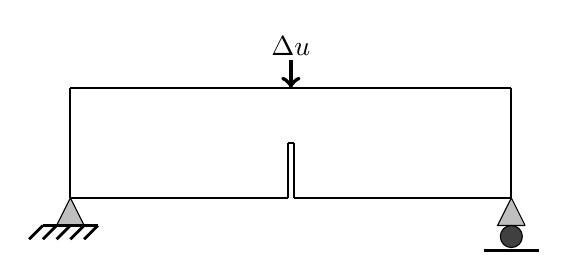
\begin{tikzpicture}[scale=0.7]
    \coordinate (K) at (0,0);
    % Square
    \draw[line width=0.75pt,black] (4,2) to (-4,2);
    \draw[line width=0.75pt,black] (4,2) to (4,0);
    \draw[line width=0.75pt,black] (4,0) to (0.05,0);
    \draw[line width=0.75pt,black] (0.05,0) to (0.05,1.0);
    \draw[line width=0.75pt,black] (0.05,1.0) to (-0.05,1.0);
    \draw[line width=0.75pt,black] (-0.05,1.0) to (-0.05,0.0);
    \draw[line width=0.75pt,black] (-0.05,0.0) to (-4.0,0.0);
    \draw[line width=0.75pt,black] (-4.0,0.0) to (-4.0,2);
    % Loading
    \draw[->,line width=1.5pt,black] (0.0,2.5) to (0.0,2.);
    \node[ ] at (0,2.75) {$\Delta\disp$};
    % Left edge
    \draw[fill=gray!50] (-4.25,-0.5) -- (-3.75,-0.5) -- (-4,0)-- (-4.25,-0.5);
    %\draw[fill=black!75] (-2.5,1.05) circle (0.2);
    \draw[line width=1pt,black] (-4.5,-0.5) to (-3.5,-0.5);
    \draw[line width=1pt,black] (-4.5,-0.5) to (-4.75,-0.75);
    \draw[line width=1pt,black] (-4.25,-0.5) to (-4.5,-0.75);
    \draw[line width=1pt,black] (-4,-0.5) to (-4.25,-0.75);
    \draw[line width=1pt,black] (-3.75,-0.5) to (-4,-0.75);
    \draw[line width=1pt,black] (-3.5,-0.5) to (-3.75,-0.75);
    % Right edge
    \draw[fill=gray!50] (4.25,-0.5) -- (3.75,-0.5) -- (4,0)-- (4.25,-0.5);
    \draw[fill=black!75] (4,-0.7) circle (0.2);
    \draw[line width=1pt,black] (4.5,-0.95) to (3.5,-0.95);
    \end{tikzpicture}
\caption{Three point bending test}
\label{sec4:fig:3pt_bending}
\end{minipage}
\hspace{0.5cm}
\begin{minipage}[b]{0.45\linewidth}
\centering
\begin{tabular}{ll} \hline
  \textbf{Parameters}  & \textbf{Value} \\ \hline
  Fracture Model & Quasi-Brittle \\
  Energy Split & Spectral \\
  Softening & Cornellisen et. al. \cite{cornelissen1986experimental} \\
  $E_0$  & 2e4 [MPa] \\
  $\nu$  & 0.2 [-] \\
  $f_t$  & 2.4 [MPa] \\
  $\gc$  & 0.113 [N/mm] \\
  $\l$  & 2.5 [mm] \\
  $\eta$ & $\beta \gc/\l$ \\ \hline
  \end{tabular}
\captionof{table}{Parameters for three point bending test}
\label{sec4:table:3pt_bending}
\end{minipage}
\end{figure}

\begin{figure}[!ht]
\centering
  \begin{subfigure}[t]{0.45\textwidth}
  \centering
    \begin{tikzpicture}[thick,scale=0.95, every node/.style={scale=1.175}]
    \begin{axis}[legend style={draw=none}, legend columns = 3,
      transpose legend, ylabel={Load\:[kN]},xlabel={Displacement\:[mm]}, xmin=0, ymin=0, xmax=1.0, ymax=1.75, yticklabel style={
        /pgf/number format/fixed,
        /pgf/number format/precision=5
        },
        scaled y ticks=false,
        xticklabel style={
        /pgf/number format/fixed,
        /pgf/number format/precision=5
        },
        scaled x ticks=false,
        every axis plot/.append style={very thick}]
    \pgfplotstableread{./Data/Rots/problem_lodi200m.dat}\Edata;
    \pgfplotstableread{./Data/Rots/problem_lodi100m.dat}\Cdata;
    \pgfplotstableread[col sep = comma]{./Data/Rots/RotsTPBUpperLodi.txt}\Bdata;
    \pgfplotstableread[col sep = comma]{./Data/Rots/RotsTPBLowerLodi.txt}\Adata;
    \addplot [name path = A, 
           color=blue!20, 
%           only marks, 
           mark=*, 
           mark size=0.25pt, 
           forget plot
         ]
         table
         [
           x expr=\thisrowno{0}, 
           y expr=\thisrowno{1}
         ] {\Adata};
    \addplot [name path = B,
           color=blue!20, 
%           only marks, 
           mark=*, 
           mark size=0.25pt, 
           forget plot
         ]
         table
         [
           x expr=\thisrowno{0}, 
           y expr=\thisrowno{1}
         ] {\Bdata};
    \addplot [blue!20, forget plot] fill between [of = A and B]; 
    \addplot [ 
           color=cyan, 
%           only marks, 
           mark=*, 
           mark size=0.05pt, 
         ]
         table
         [
           x expr=\thisrowno{0}, 
           y expr=\thisrowno{1}
         ] {\Cdata};
         \addlegendentry{100}
    \addplot [ 
           color=magenta, 
%           only marks, 
           mark=*, 
           mark size=0.05pt, 
         ]
         table
         [
           x expr=\thisrowno{0}, 
           y expr=\thisrowno{1}
         ] {\Edata};
         \addlegendentry{200} 
    \end{axis}
    \end{tikzpicture}
    \caption{Load-displacement plot}
    \label{sec4:fig:3pt_bending_lodi}
  \end{subfigure}
  \hspace{5mm}
  %
  \begin{subfigure}[t]{0.45\textwidth}
  \centering
    \begin{tikzpicture}
    \node[inner sep=0pt] () at (0,0)
    {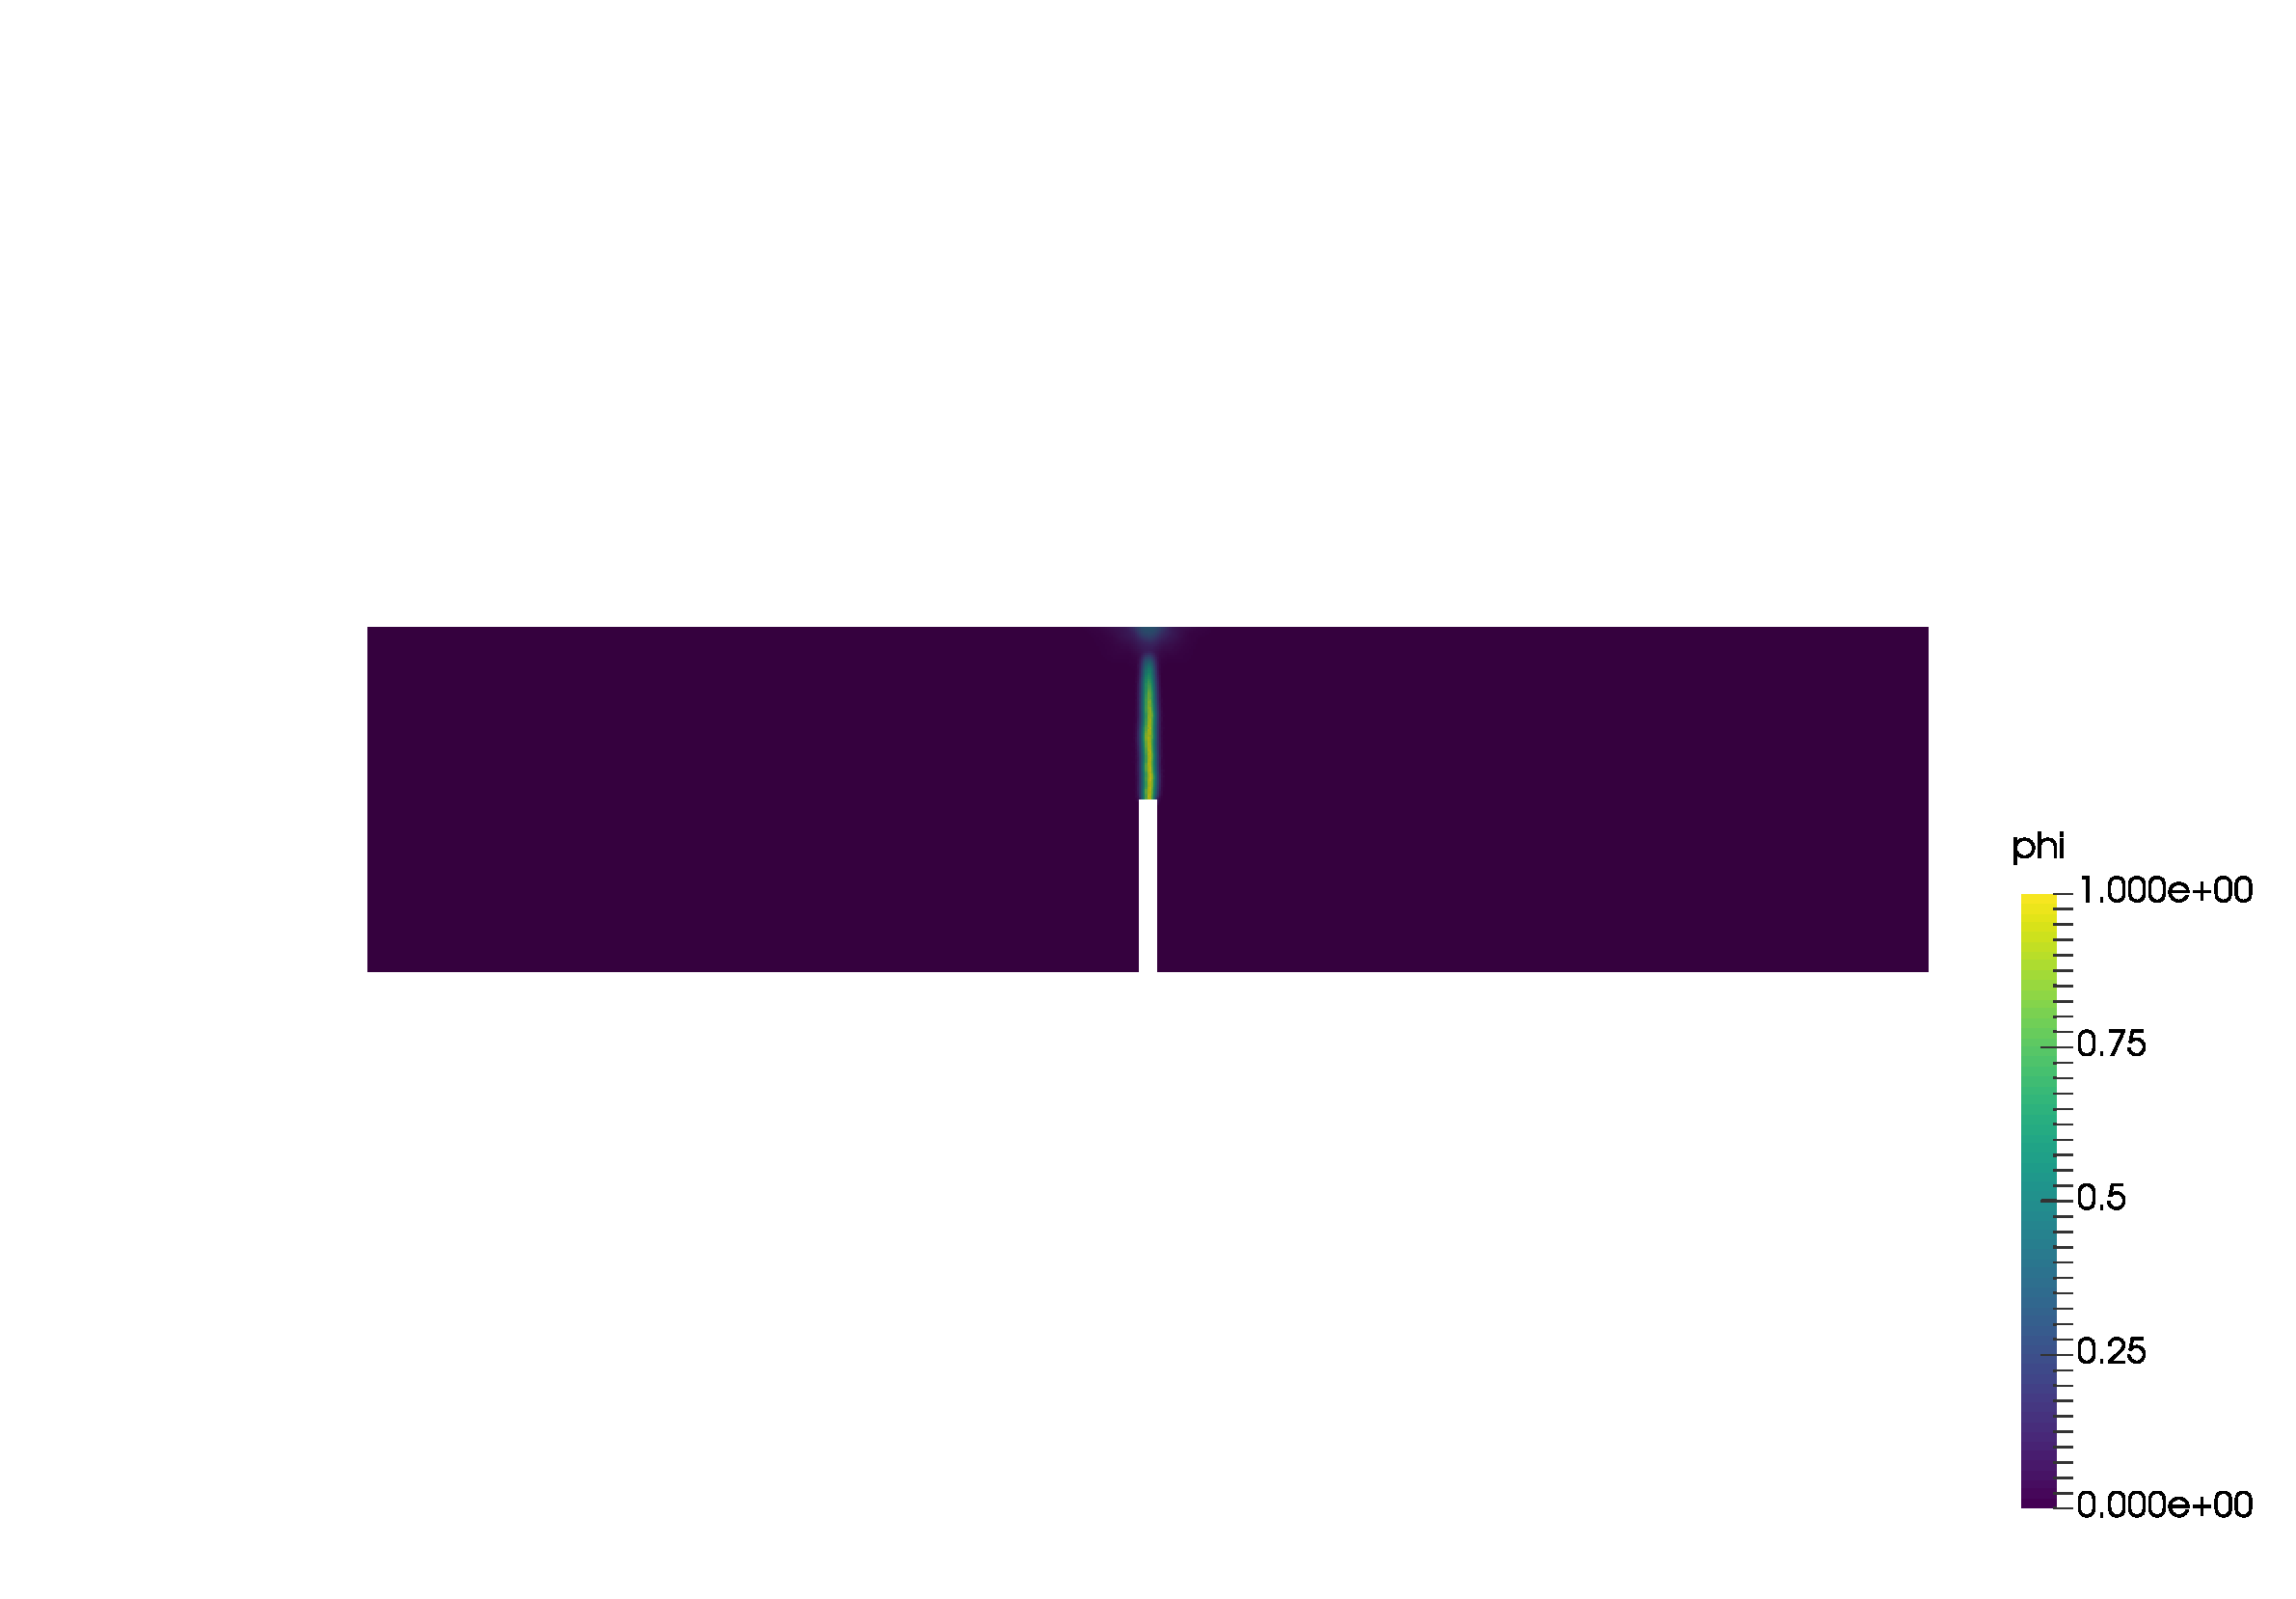
\includegraphics[width=6.0cm,trim=7cm 1cm 7cm 1cm, clip]{Images/RotsTPB/rots_pf.pdf}};
    \node[inner sep=0pt] () at (-1.2,-1.75)
    {\begin{axis}[
    hide axis,
    scale only axis,
    height=0pt,
    width=0pt,
    colormap/viridis,
    colorbar horizontal,
    point meta min=0,
    point meta max=1,
    colorbar style={
        width=4.75cm,
        xtick={0,0.5,1.0},
        xticklabel style = {yshift=-0.075cm}
    }]
    \addplot [draw=none] coordinates {(0,0)};
    \end{axis}};
    \node[inner sep=0pt] () at (0,-2.45) {$\pf$};
    \end{tikzpicture}
    \caption{ }
    \label{sec4:fig:pf_3pt_bending_failure}
  \end{subfigure}
  \caption{Figure (a) presents the load-displacement curves for the concrete three-point bending test, with $\beta = 100, 200$. The experimental range is represented by the shaded area. Figure (b) shows the distribution of the phase-field variable at the final step of the analysis in a section of the beam.}
  \label{sec4:fig:3pt_bending_results}
\end{figure}

Figure \ref{sec4:fig:3pt_bending_lodi} presents the load-displacement curves using the micromorphic phase-field fracture model, with $\beta = 100,200$. The range of the experimentally obtained load-displacement curves is exhibited by the shaded region. For both values of $\beta$, the load-displacement curves exhibit a good agreement with the experimental region. Moreover, the phase-field topology in the final step of the simulation in Figure \ref{sec4:fig:pf_3pt_bending_failure} is similar to that from the literature \cite{Rots1988}.

\subsection{Hydraulic fracturing}\label{sec4:HydFrac}

Two numerical experiments, adopted from \cite{Mikelic2015fluidfrac} are considered for simulating hydraulic fracturing. The geometry consists on a square ($2 \times 2$ [m$^2$]) embedded with a Single Natural Fracture (SNF) in Figure \ref{sec4:fig:snc} and Three Natural Fractures (TNF) in Figure \ref{sec4:fig:tnc}. The fracture in the SNF specimen has a length $0.4$ [m] and is located midway along the height. In the TNF specimen, two additional fractures are introduced. The vertical fracture has a length $1$ [m] and is located at an x-offset $0.6$ [m] from the centre of the specimen. The third fracture is a line segment from coordinates (-0.8,-0.3) to (-0.3,-0.8) assuming the axes origin placed at the centre of the specimen. Furthermore, on the external boundaries of the SNF and TNF models, the displacements and the fluid flux are set to zero. fluid is injected into the existing fractures (shown in red in Figures \ref{sec4:fig:snc} and \ref{sec4:fig:tnc}) at a rate $q^p$. Note that in \cite{Mikelic2015fluidfrac}, the fluid injection is carried out using a point source instead of a line source. The model parameters, required for the simulation, are presented in Table \ref{sec4:table:hydfracparams}.

\begin{figure}[ht]
\begin{minipage}[b]{0.3\linewidth}
\centering
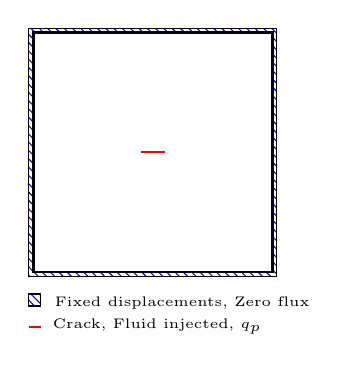
\begin{tikzpicture}[scale=0.75]
    \coordinate (K) at (0,0);
    % Fixity
    \draw[pattern=north west lines, pattern color=blue,line width=0.5pt] (-2.1,-2.1) rectangle (2.1,2.1);
    % Rectangle
    \draw[line width=1.0pt,black,fill=white] ( -2.025,-2.025) rectangle (2.025,2.025);    
    % Natural Fractures
    \draw[line width=0.75pt,red] (-0.2,0) to (0.2,0);
    % Label
    \draw[pattern=north west lines, pattern color=blue,line width=0.5pt] (-2.1,-2.6) rectangle (-1.9,-2.4);
    \node[ ] at (0.5,-2.55) {\tiny{Fixed displacements, Zero flux}};
    \draw[line width=0.75pt,red] (-2.1,-2.95) to (-1.9,-2.95);
    \node[ ] at (0.075,-2.95) {\tiny{Crack, Fluid injected, $q_p$}};
    \end{tikzpicture}
\caption{Single natural fracture}
\label{sec4:fig:snc}
\end{minipage}
\begin{minipage}[b]{0.3\linewidth}
\centering
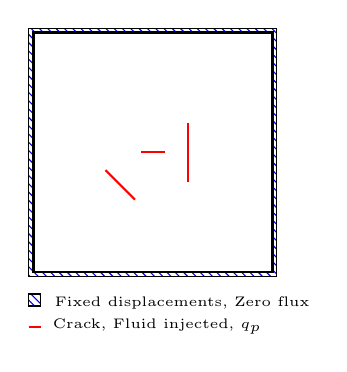
\begin{tikzpicture}[scale=0.75]
    \coordinate (K) at (0,0);
    % Fixity
    \draw[pattern=north west lines, pattern color=blue,line width=0.5pt] (-2.1,-2.1) rectangle (2.1,2.1);
    % Rectangle
    \draw[line width=1.0pt,black,fill=white] ( -2.025,-2.025) rectangle (2.025,2.025);    
    % Natural Fractures
    \draw[line width=0.75pt,red] (-0.2,0) to (0.2,0);
    \draw[line width=0.75pt,red] (0.6,-0.5) to (0.6,0.5);
    \draw[line width=0.75pt,red] (-0.8,-0.3) to (-0.3,-0.8);
    % Label
    \draw[pattern=north west lines, pattern color=blue,line width=0.5pt] (-2.1,-2.6) rectangle (-1.9,-2.4);
    \node[ ] at (0.5,-2.55) {\tiny{Fixed displacements, Zero flux}};
    \draw[line width=0.75pt,red] (-2.1,-2.95) to (-1.9,-2.95);
    \node[ ] at (0.075,-2.95) {\tiny{Crack, Fluid injected, $q_p$}};
    \end{tikzpicture}
\caption{Three natural fractures}
\label{sec4:fig:tnc}
\end{minipage}
\begin{minipage}[b]{0.3\linewidth}
\centering
\scriptsize
\begin{tabular}{ll} \hline
  \textbf{Parameters} & \textbf{Value} \\ \hline
  Fracture Model & AT2 \\
  Energy Split & Spectral Split \\
  $E_0$ & 1 [GPa] \\
  $\nu$ & 0.2 [-] \\
  $\gc$ & 1 [N/m] \\
  $\l$ & 5e-2 [m] \\
  $\alpha$ & 1.0 [-] \\
  $n$ & 0.3 [-] \\
  $k_{i,b}$ & 1e-12 [m$^2$] \\
  $\mu_f$ & 1e-3 [Pa\,s] \\
  $K_s$ & 1 [GPa] \\ 
  $K_f$ & 40 [MPa]\\
  $q^p$ & 0.01 [m/s] \\
  $\eta$ & $200 \gc/\l$ \\ \hline
  \end{tabular}
\captionof{table}{Model parameters}
\label{sec4:table:hydfracparams}
\end{minipage}
\end{figure}

Figure \ref{sec4:fig:snf_pf} presents the distribution of the phase-field in the SNF specimen at different times ( $t = 0.01$, $0.1$ and $0.2$ [s]) during the fluid driven fracture propagation simulation. A similar fracture topology compared to \cite{Mikelic2015fluidfrac} has been observed. Furthermore, the corresponding fluid pressure distributions are presented in Figure \ref{sec4:fig:snf_pres}. The localization of the fluid pressure follows from the dual permeability model (see Section \ref{sec:hydfracEFuncTransport}), wherein the intrinsic permeability in the fracture is larger than the intrinsic permeability of the bulk material. Furthermore, as reported in \cite{Mikelic2015fluidfrac}, negative fluid pressure values are observed at the fracture tips, throughout the simulation.

\begin{figure}[!ht]
\centering
  \begin{subfigure}[t]{0.275\textwidth}
  \centering
    \begin{tikzpicture}
    \node[inner sep=0pt] () at (0,0)
    {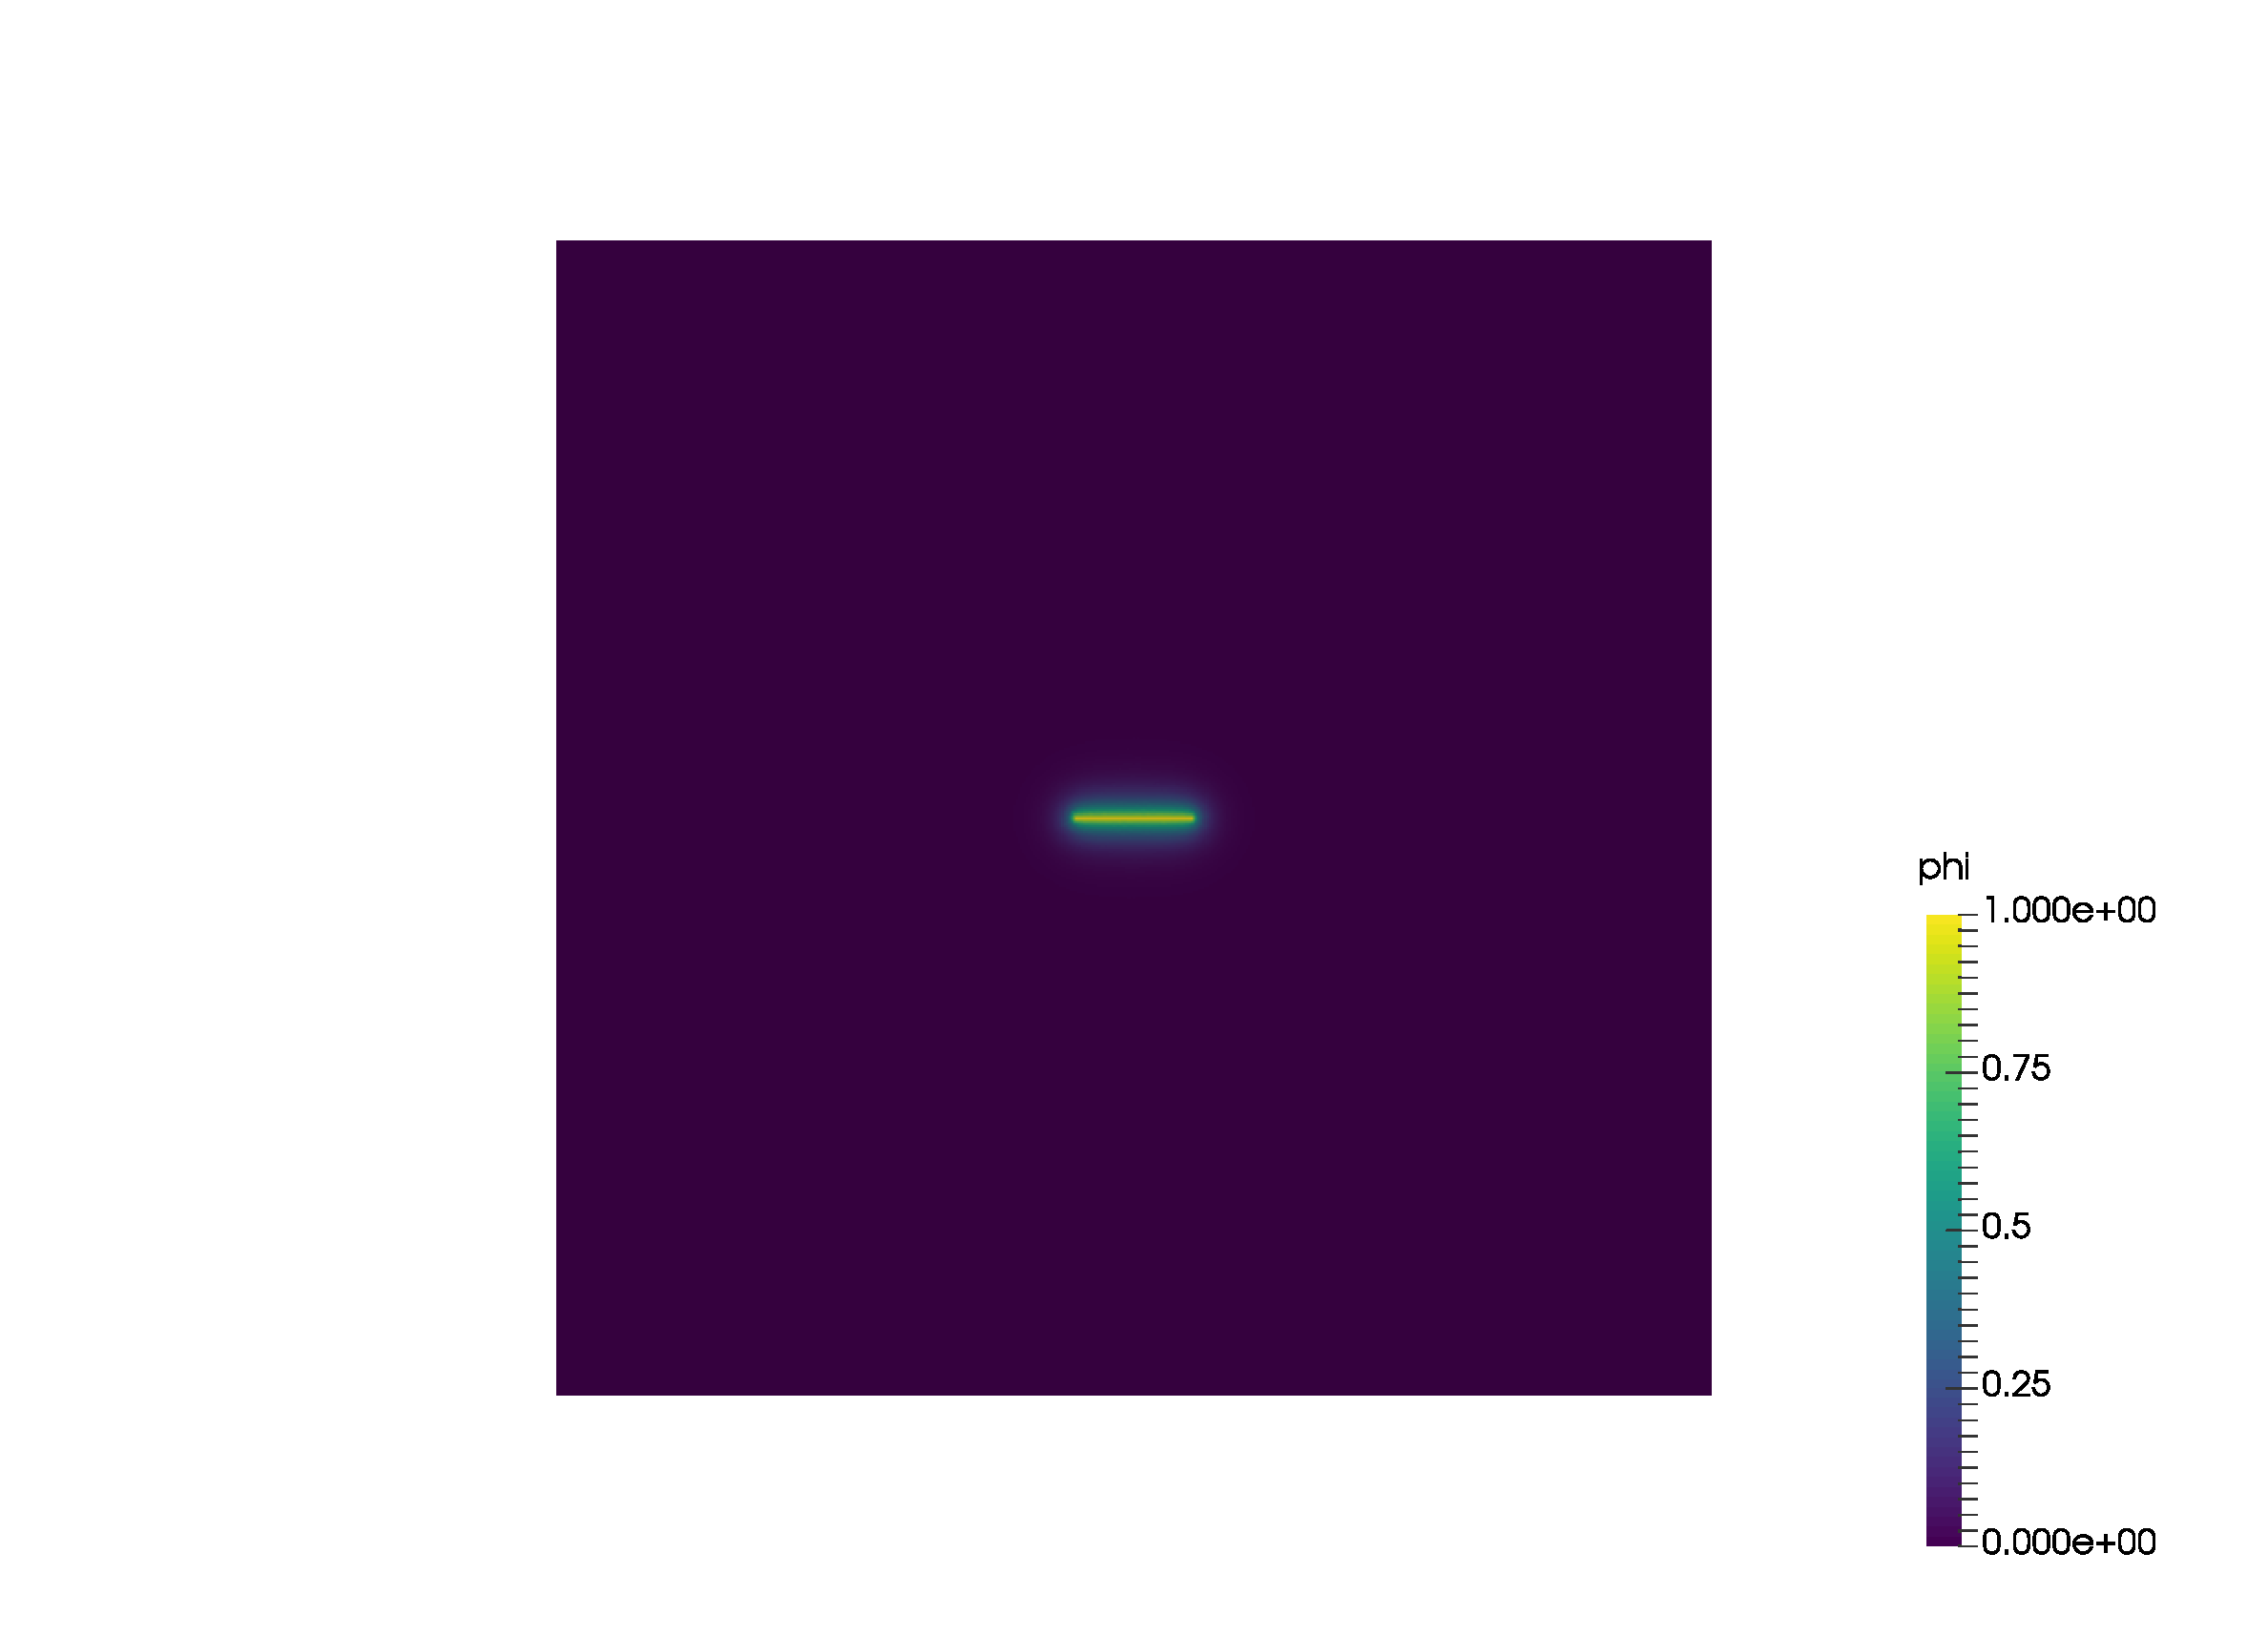
\includegraphics[width=5cm,trim=7cm 1cm 7cm 1cm, clip]{Images/SNF/snf_d_0_0.pdf}};
    \end{tikzpicture}
    \caption{t = 0.01 [s]}
    \label{sec4:fig:snf_d_0_0}
  \end{subfigure}
  \hspace{2.5mm}
  \begin{subfigure}[t]{0.275\textwidth}
  \centering
    \begin{tikzpicture}
    \node[inner sep=0pt] () at (0,0)
    {\includegraphics[width=5cm,trim=7cm 1cm 7cm 1cm, clip]{Images/SNF/snf_d_0_1.pdf}};
    \end{tikzpicture}
    \caption{t = 0.1 [s]}
    \label{sec4:fig:snf_d_0_1}
  \end{subfigure}
  \hspace{2.5mm}
  \begin{subfigure}[t]{0.275\textwidth}
  \centering
    \begin{tikzpicture}
    \node[inner sep=0pt] () at (0,0)
    {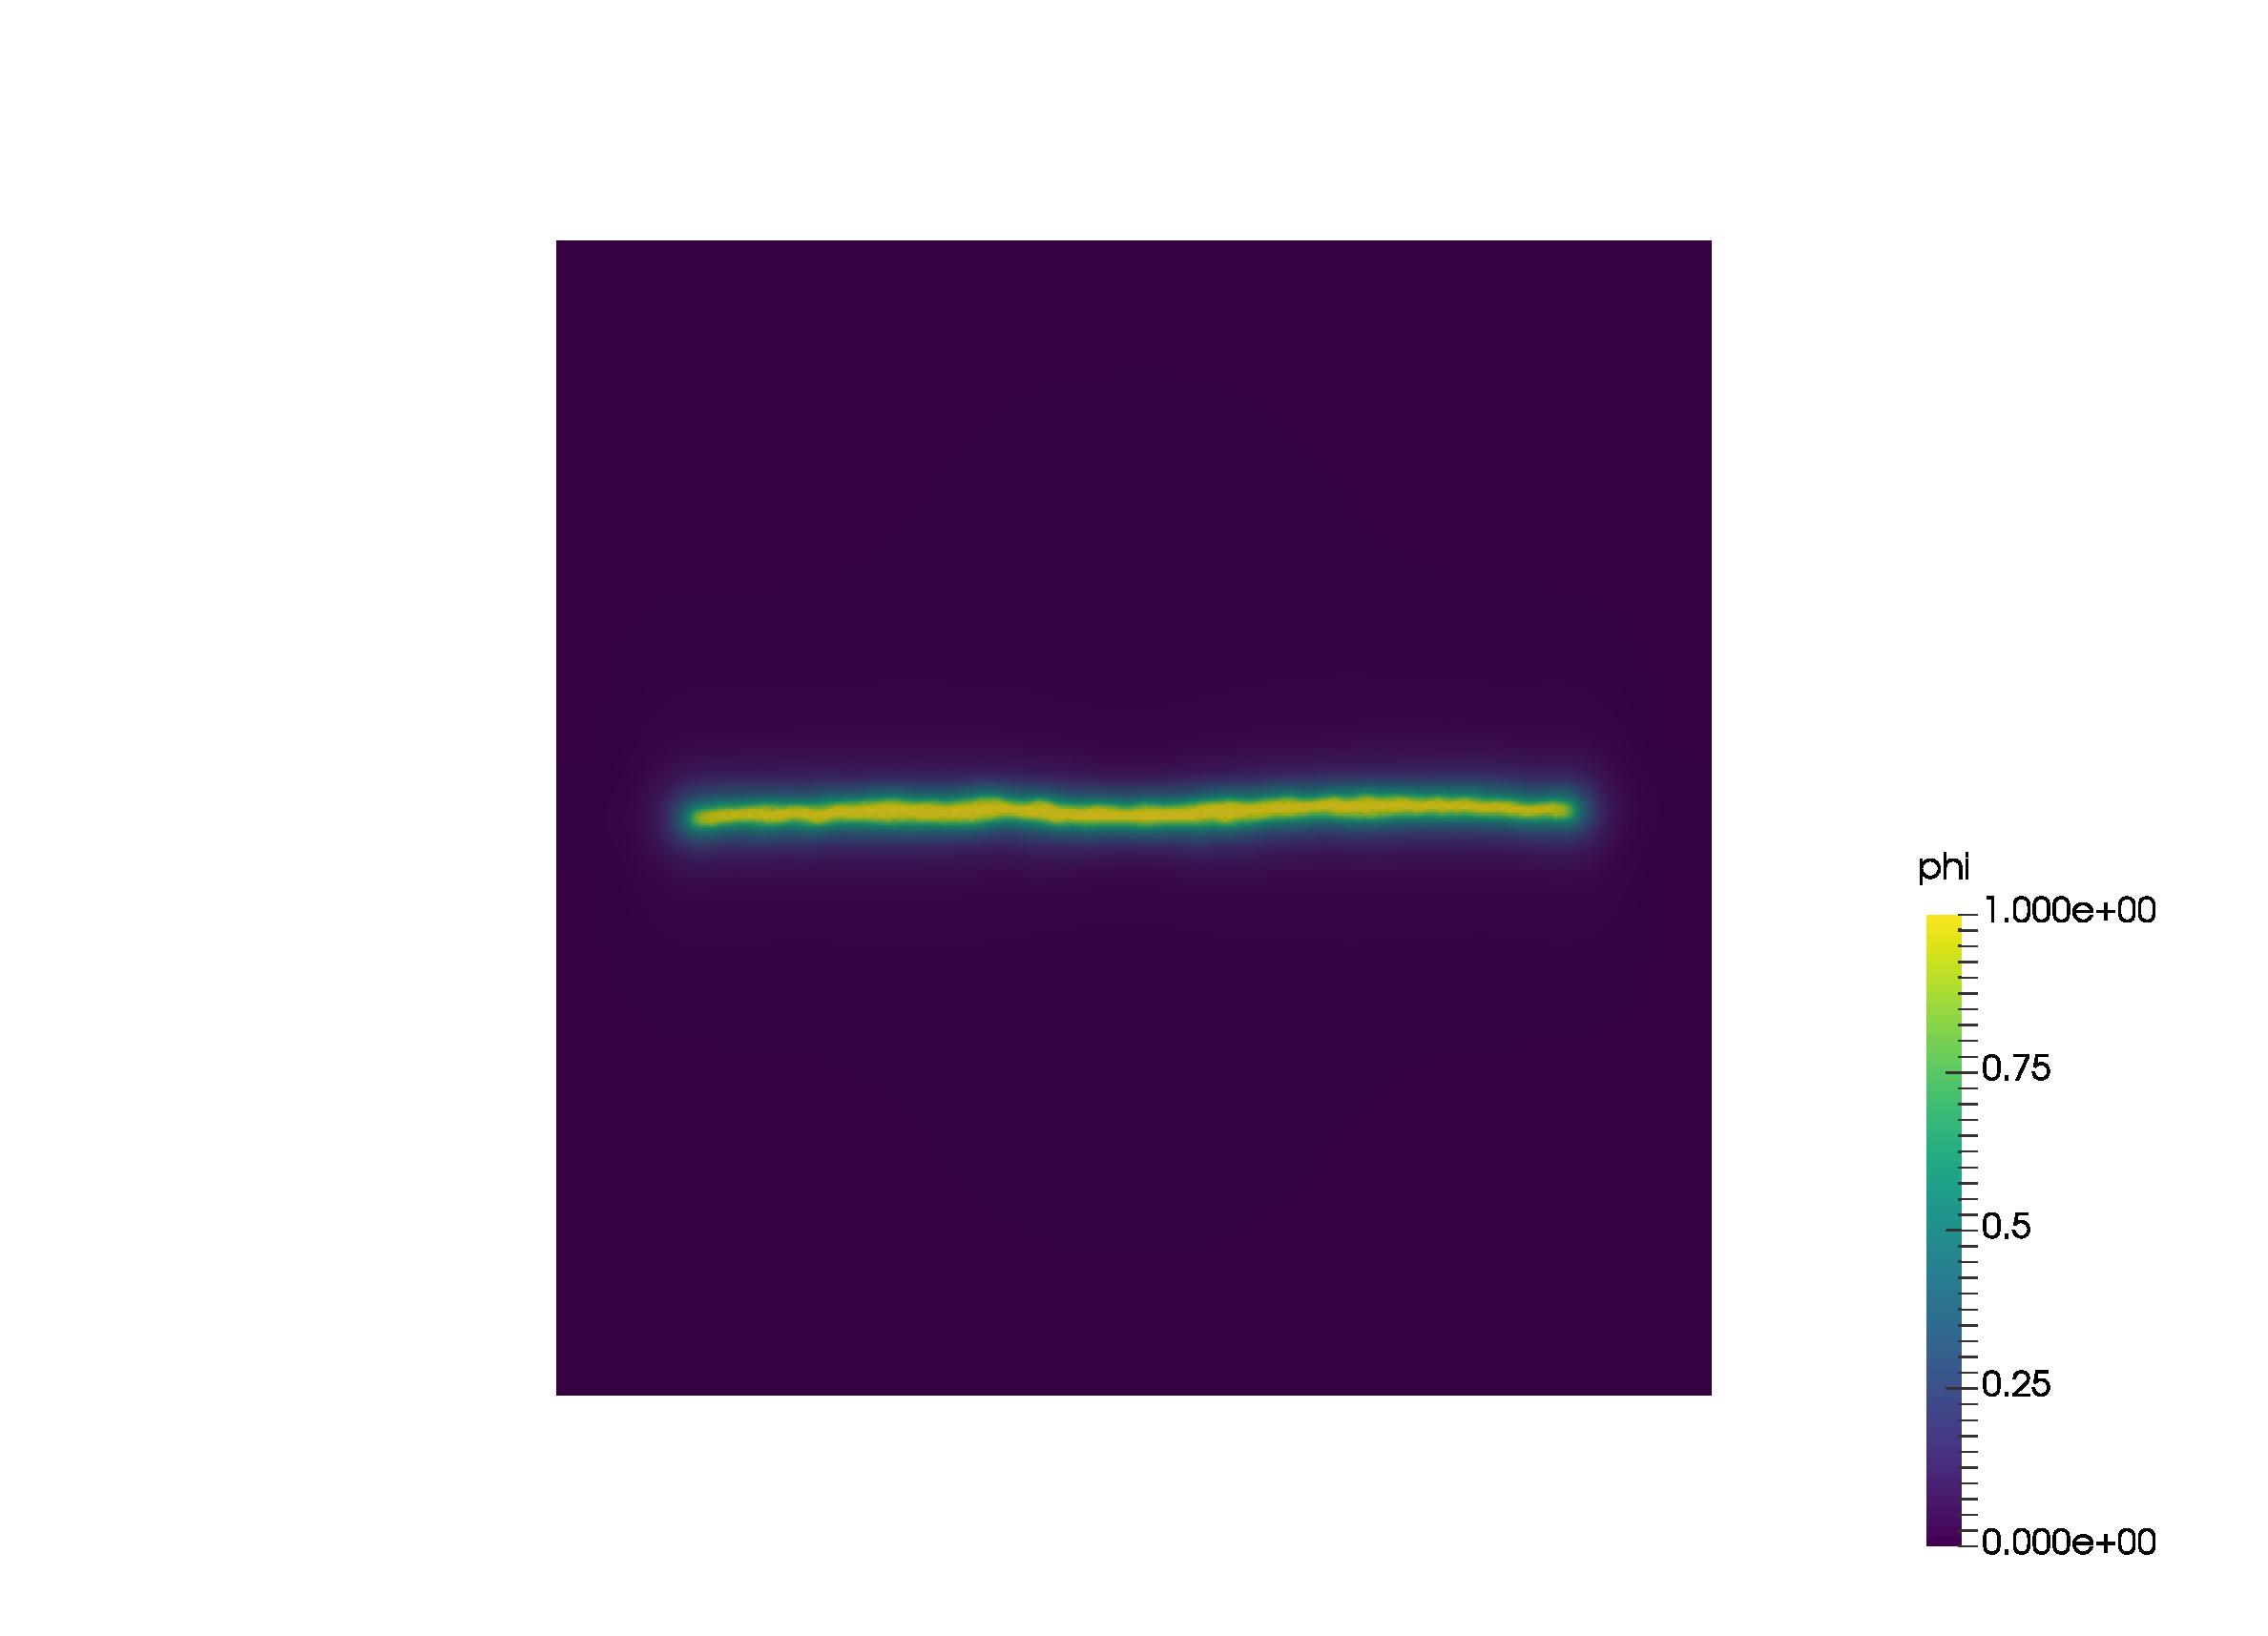
\includegraphics[width=5cm,trim=7cm 1cm 7cm 1cm, clip]{Images/SNF/snf_d_0_2.pdf}};
    \end{tikzpicture}
    \caption{t = 0.2 [s]}
    \label{sec4:fig:snf_d_0_2}
  \end{subfigure}
  \hspace{0.5mm}
  \begin{subfigure}[t]{0.05\textwidth}
  \setlength{\unitlength}{1pt}
    \begin{picture}(1,1)
    \put(-80.,-16){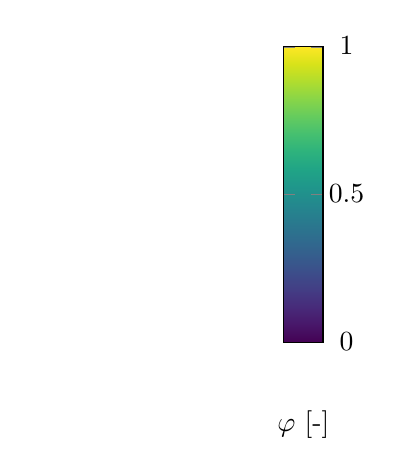
\begin{tikzpicture}[rotate=0]
    {\begin{axis}[
    hide axis,
    scale only axis,
    height=0pt,
    width=0pt,
    colormap/viridis,
    colorbar horizontal,
    point meta min=0,
    point meta max=1,
    colorbar style={
        width=3.75cm,
        rotate=90,
        at={(0.0,50.0)},anchor=south,   
        xtick={0,0.5,1.0},
        xticklabel style = {yshift=0.25cm},
        xticklabel style = {xshift=0.3cm}
    }]
    %\addplot [draw=none] coordinates {(1.5,0)};
    \end{axis}};
    \node[inner sep=0pt] () at (0,-1.05) {$\pf$ [-]};
    \end{tikzpicture}}
    \end{picture}
  \end{subfigure}
  \caption{Figures (a-c) present the distribution of the phase-field variable at the different times during the analysis of the Single Natural Fracture (SNF) specimen.}
  \label{sec4:fig:snf_pf}
\end{figure}

\clearpage

\begin{figure}[!ht]
\centering
  \begin{subfigure}[t]{0.275\textwidth}
  \centering
    \begin{tikzpicture}
    \node[inner sep=0pt] () at (0,0)
    {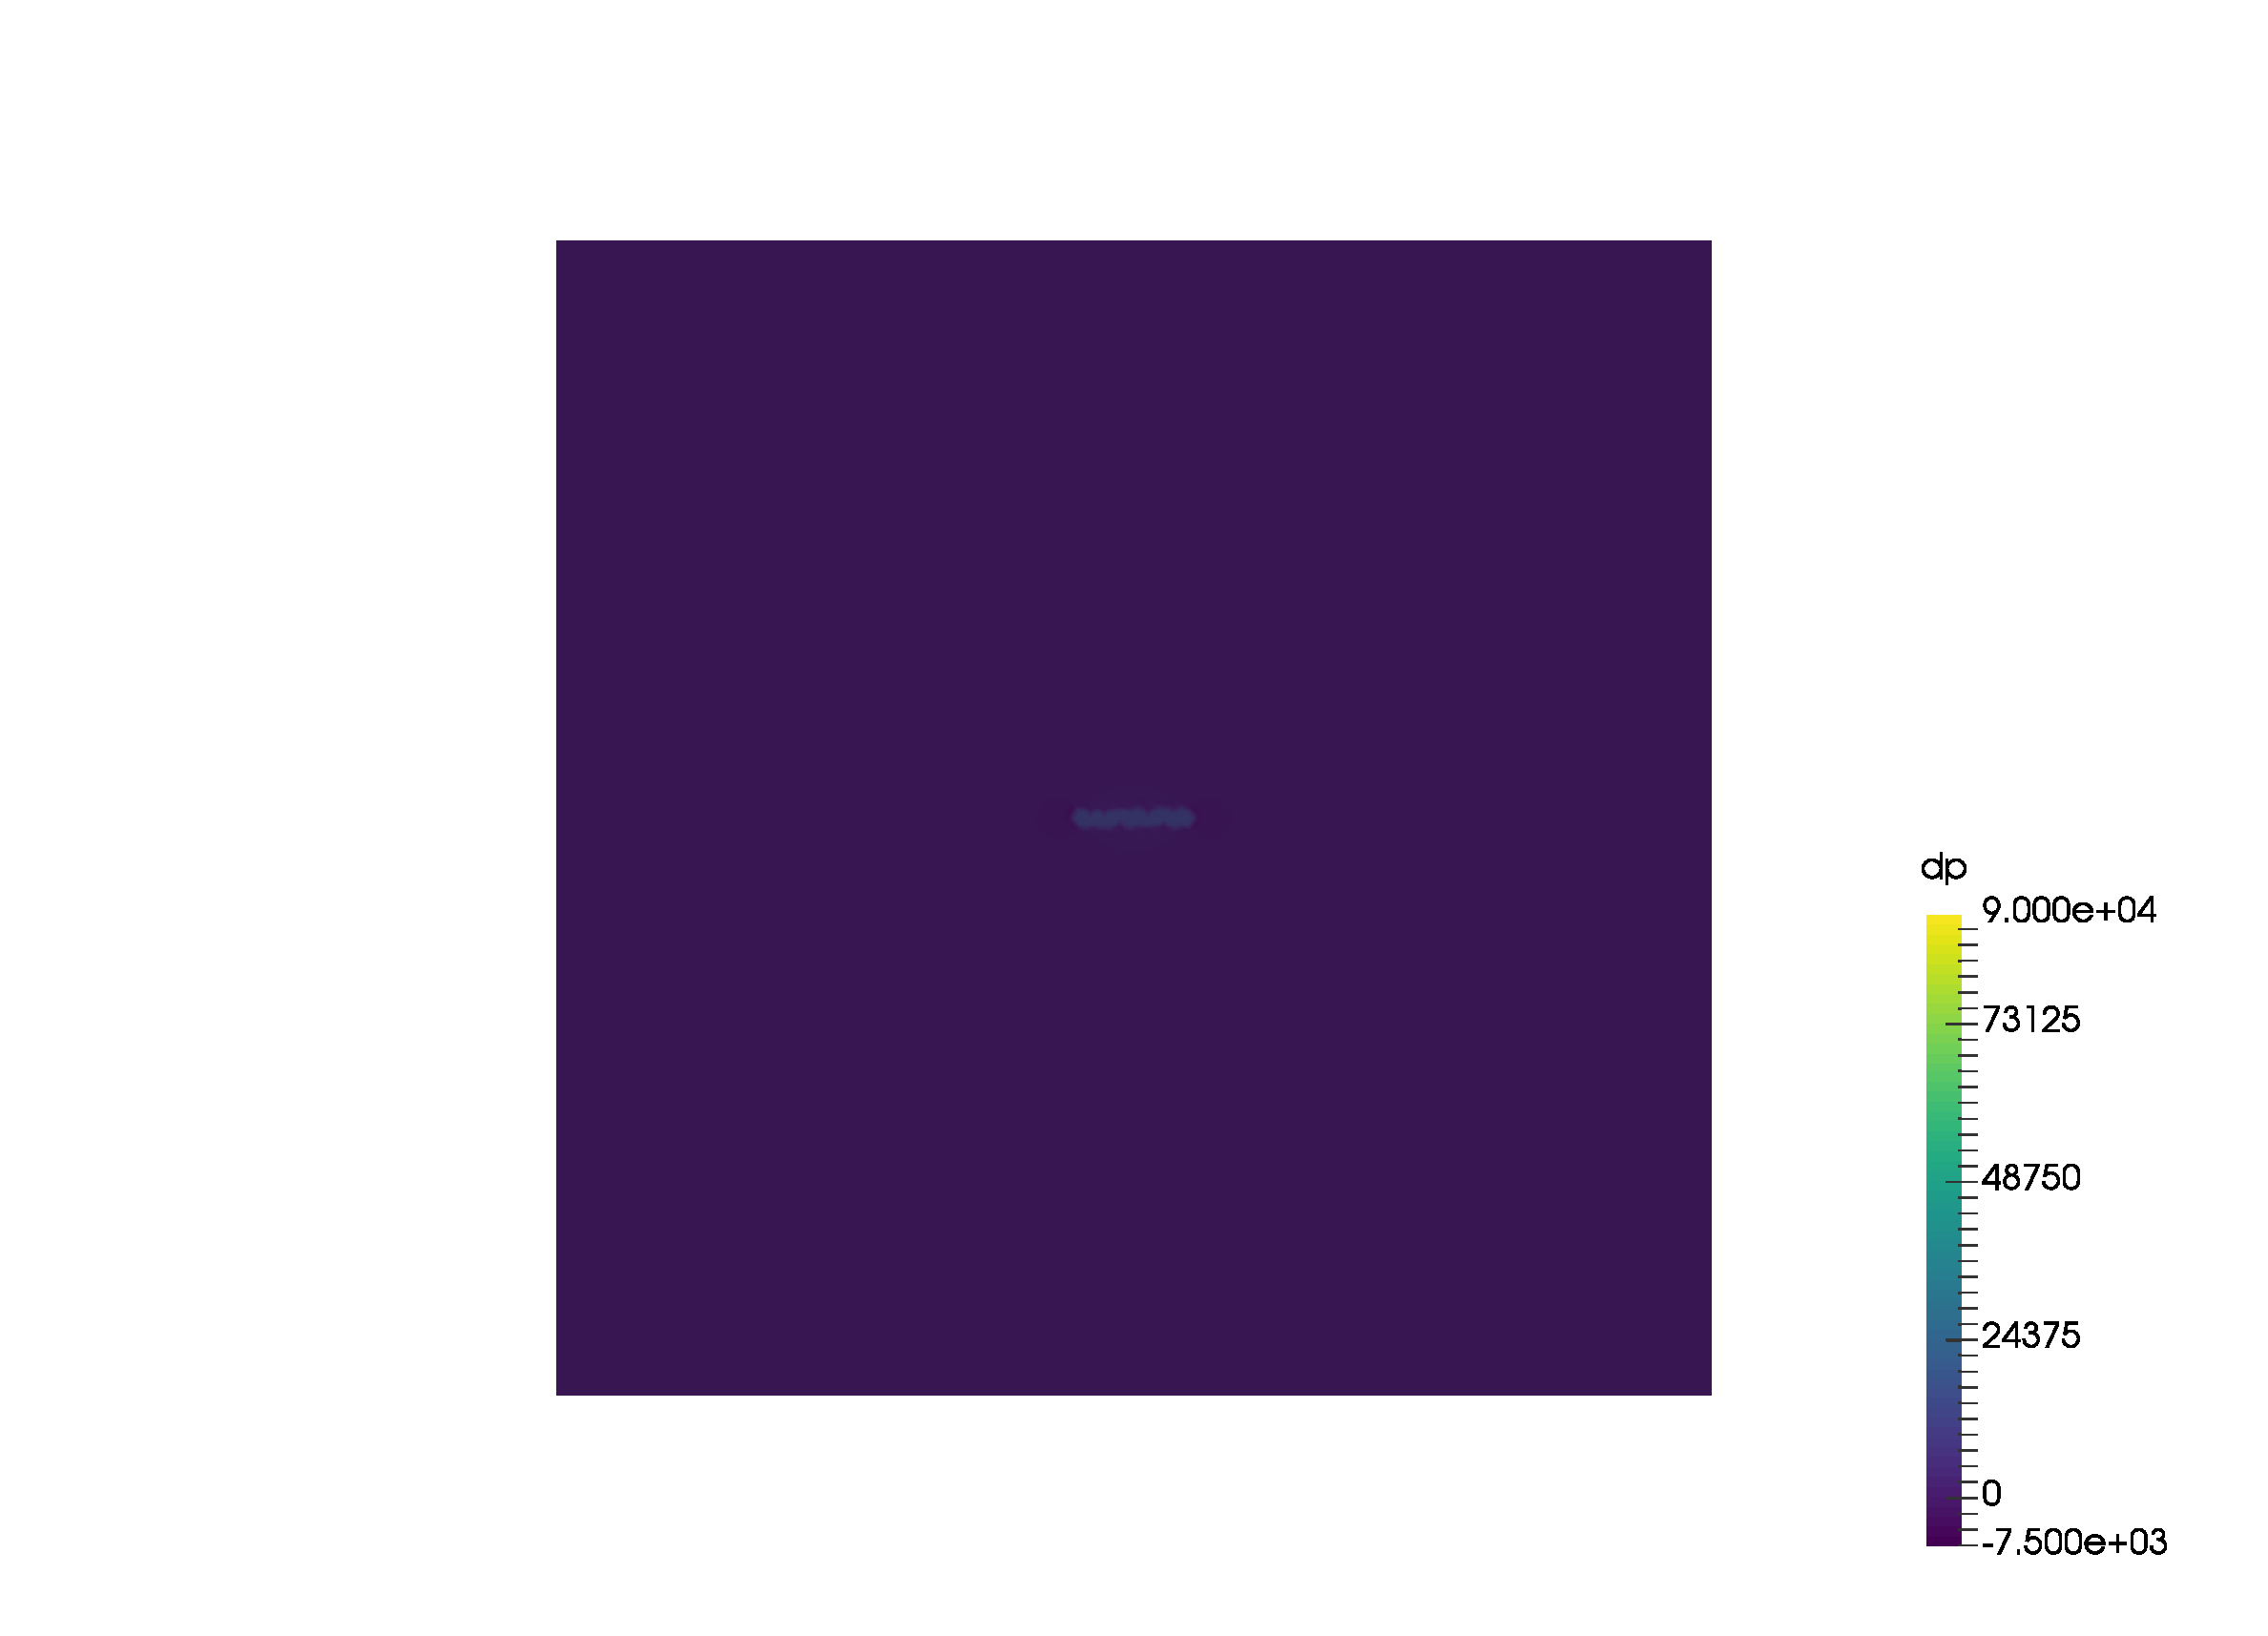
\includegraphics[width=5cm,trim=7cm 1cm 7cm 1cm, clip]{Images/SNF/snf_p_0_0.pdf}};
    \end{tikzpicture}
    \caption{t = 0.01 [s]}
    \label{sec4:fig:snf_p_0_0}
  \end{subfigure}
  \hspace{2.5mm}
  \begin{subfigure}[t]{0.275\textwidth}
  \centering
    \begin{tikzpicture}
    \node[inner sep=0pt] () at (0,0)
    {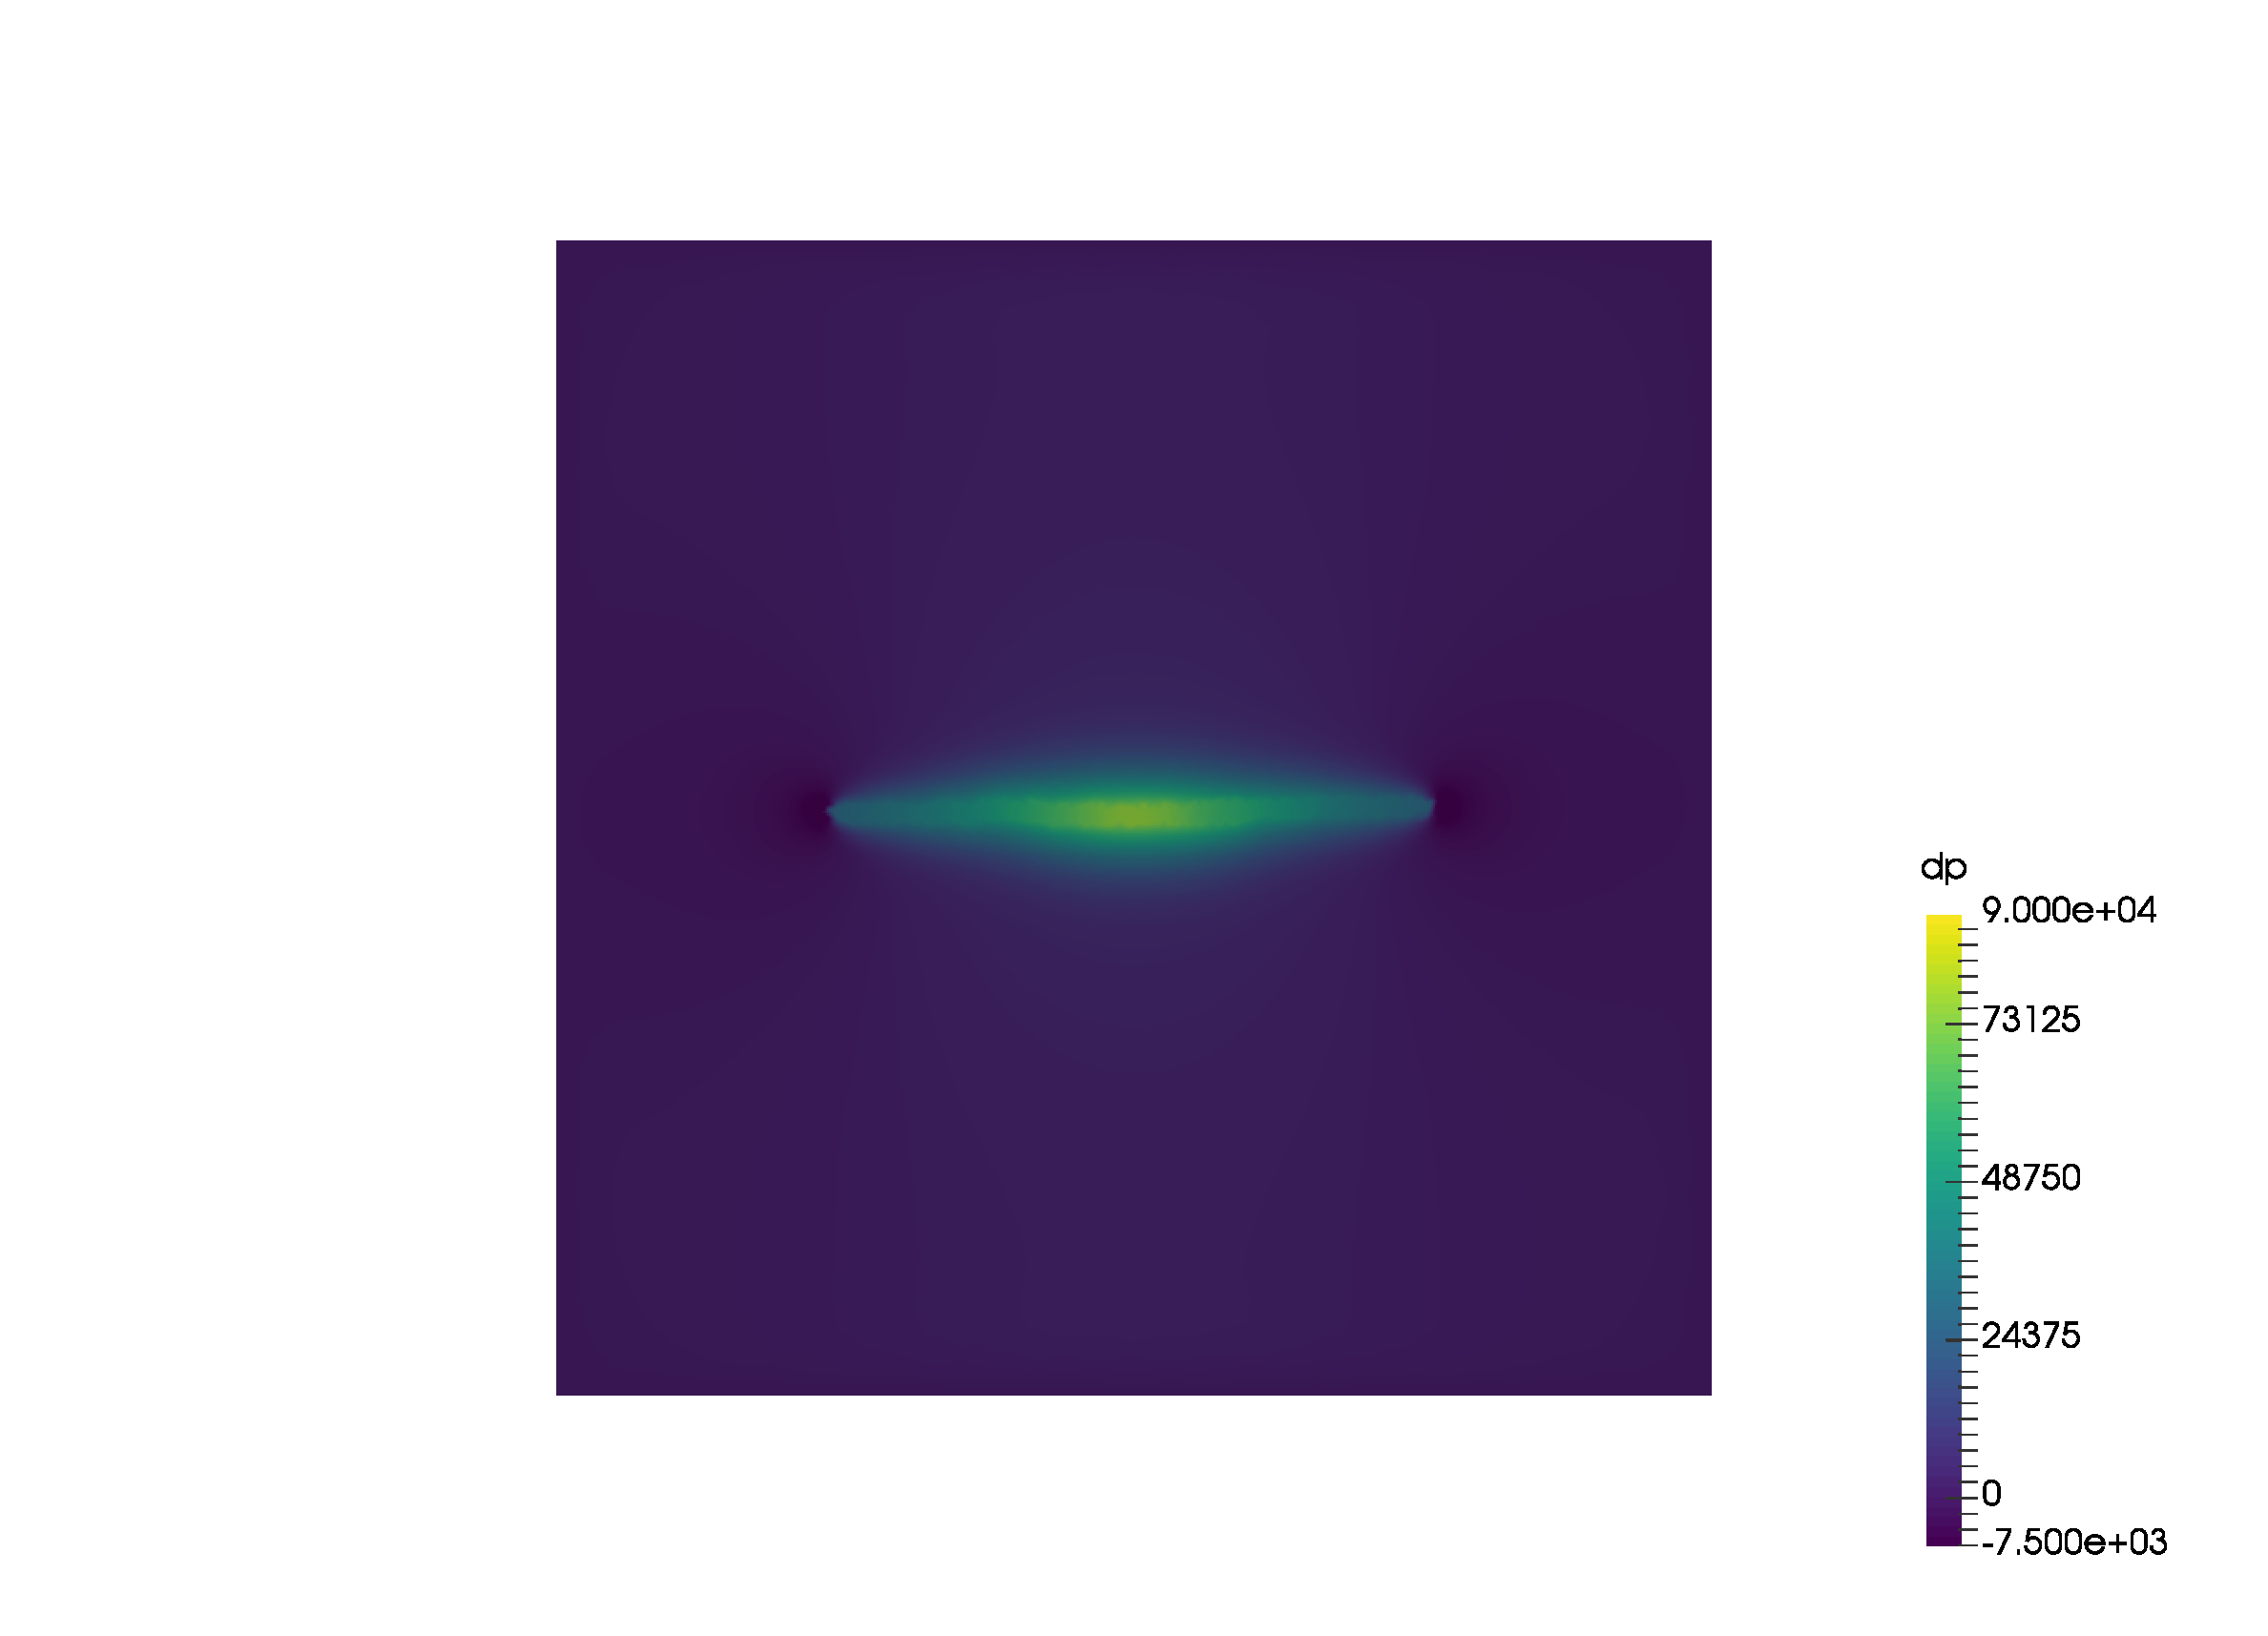
\includegraphics[width=5cm,trim=7cm 1cm 7cm 1cm, clip]{Images/SNF/snf_p_0_1.pdf}};
    \end{tikzpicture}
    \caption{t = 0.1 [s]}
    \label{sec4:fig:snf_p_0_1}
  \end{subfigure}
  \hspace{2.5mm}
  \begin{subfigure}[t]{0.275\textwidth}
  \centering
    \begin{tikzpicture}
    \node[inner sep=0pt] () at (0,0)
    {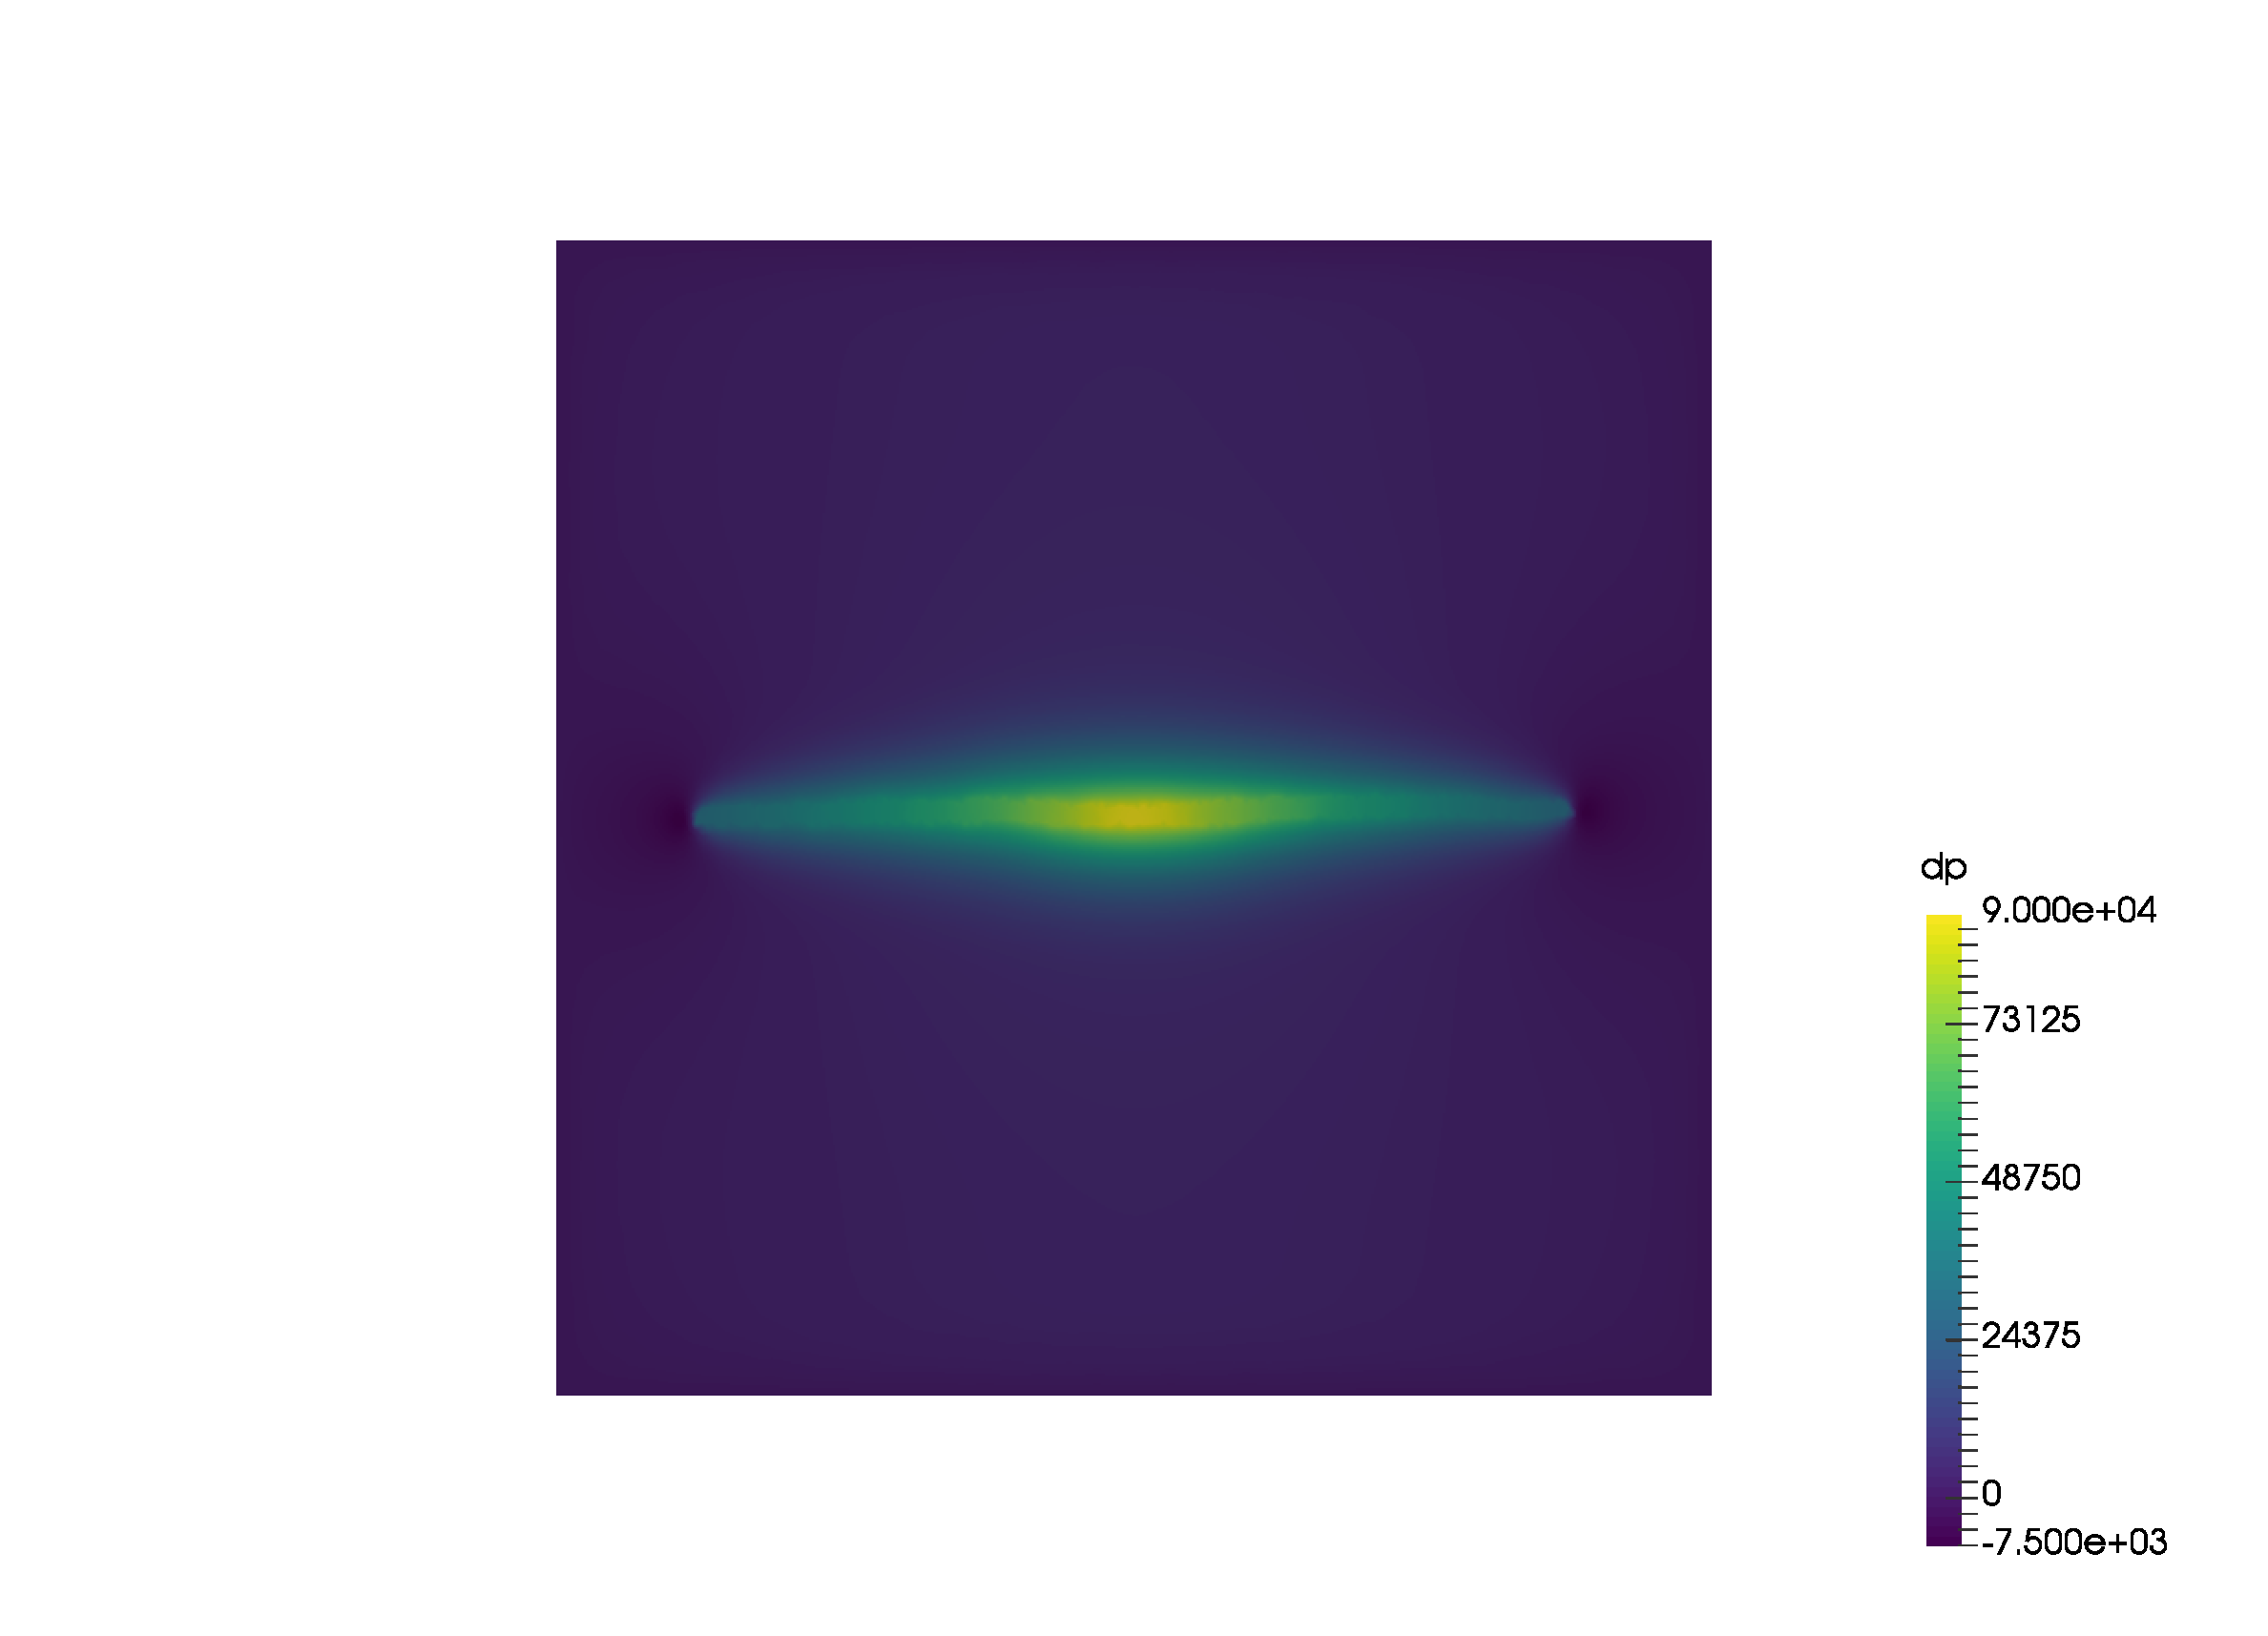
\includegraphics[width=5cm,trim=7cm 1cm 7cm 1cm, clip]{Images/SNF/snf_p_0_2.pdf}};
    \end{tikzpicture}
    \caption{t = 0.2 [s]}
    \label{sec4:fig:snf_p_0_2}
  \end{subfigure}
  \hspace{0.5mm}
  \begin{subfigure}[t]{0.05\textwidth}
  \setlength{\unitlength}{1pt}
    \begin{picture}(1,1)
    \put(-80.,-16){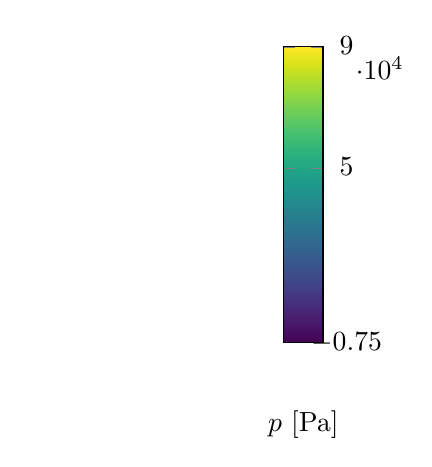
\begin{tikzpicture}[rotate=0]
    {\begin{axis}[
    hide axis,
    scale only axis,
    height=0pt,
    width=0pt,
    colormap/viridis,
    colorbar horizontal,
    point meta min=-7500,
    point meta max=90000,
    colorbar style={
        width=3.75cm,
        rotate=90,
        at={(0.0,50.0)},anchor=south,   
        xtick={-7500,50000,90000},
        xticklabel style = {yshift=0.25cm},
        xticklabel style = {xshift=0.3cm}
    }]
    %\addplot [draw=none] coordinates {(1.5,0)};
    \end{axis}};
    \node[inner sep=0pt] () at (0,-1.05) {$p$ [Pa]};
    \end{tikzpicture}}
    \end{picture}
  \end{subfigure}
  \caption{Figures (a-c) present the distribution of the fluid pressure at the different times during the analysis of the Single Natural Fracture (SNF) specimen.}
  \label{sec4:fig:snf_pres}
\end{figure}

Next, the TNF specimen is presented in this manuscript to demonstrate the fracture merging capabilities of the micromorphic phase-field fracture model. To this end, Figure \ref{sec4:fig:tnf_pf} presents the distribution of the phase-field in the SNF specimen at different times ( $t = 0.001$, $0.024$ and $0.048$ [s]) during the fluid driven fracture propagation simulation. Figure \ref{sec4:fig:tnf_d_0_024} illustrates the merging of the evolving phase-field from the horizontal fracture onto the vertical fracture. In the same figure, the phase-field from the horizontal fracture evolves leftwards in a curved fashion subsequently merging with the inclined fracture, as shown in Figure \ref{sec4:fig:tnf_d_0_048}. Furthermore, owing to the dual permeability model, localized fluid pressure distributions are observed in Figure \ref{sec4:fig:tnf_pres}. Similar observations were made in \cite{Mikelic2015fluidfrac} albeit with a point source of fluid injection, and a different dual permeability relationship.

\begin{figure}[!ht]
\centering
  \begin{subfigure}[t]{0.275\textwidth}
  \centering
    \begin{tikzpicture}
    \node[inner sep=0pt] () at (0,0)
    {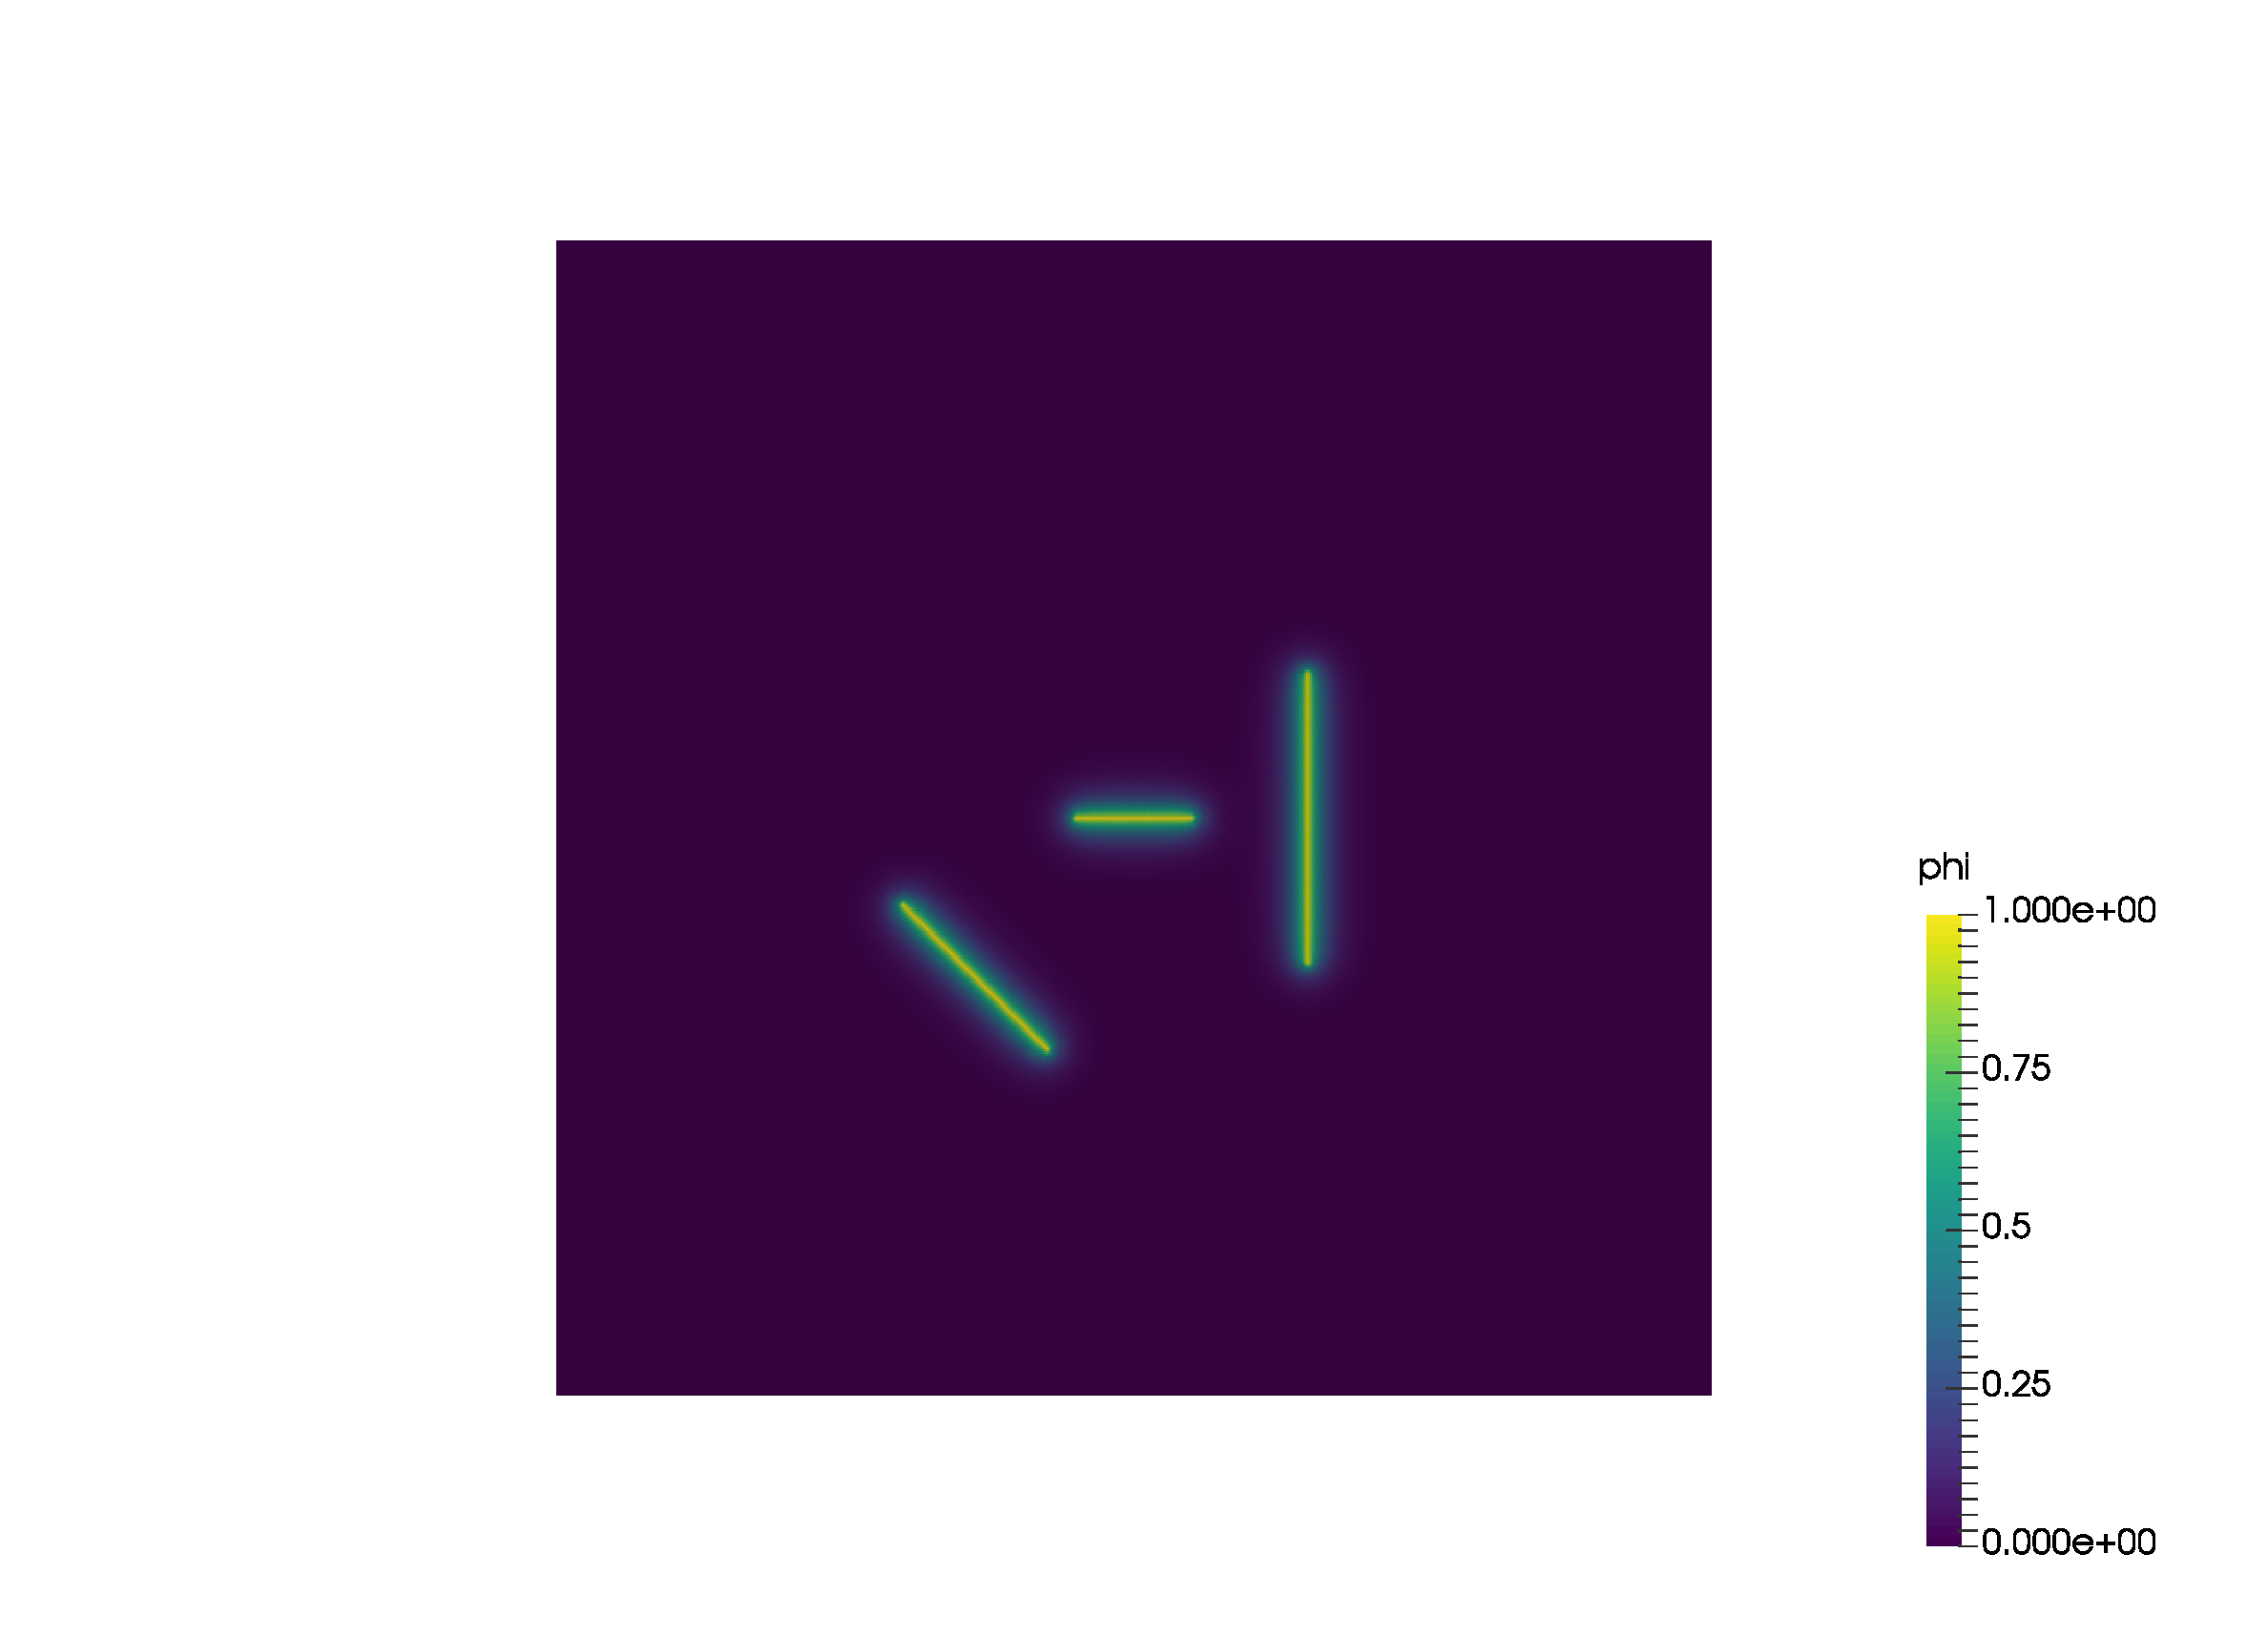
\includegraphics[width=5cm,trim=7cm 1cm 7cm 1cm, clip]{Images/TNF/tnf_d_0_0.pdf}};
    \end{tikzpicture}
    \caption{t = 0.001 [s]}
    \label{sec4:fig:tnf_d_0_0}
  \end{subfigure}
  \hspace{2.5mm}
  \begin{subfigure}[t]{0.275\textwidth}
  \centering
    \begin{tikzpicture}
    \node[inner sep=0pt] () at (0,0)
    {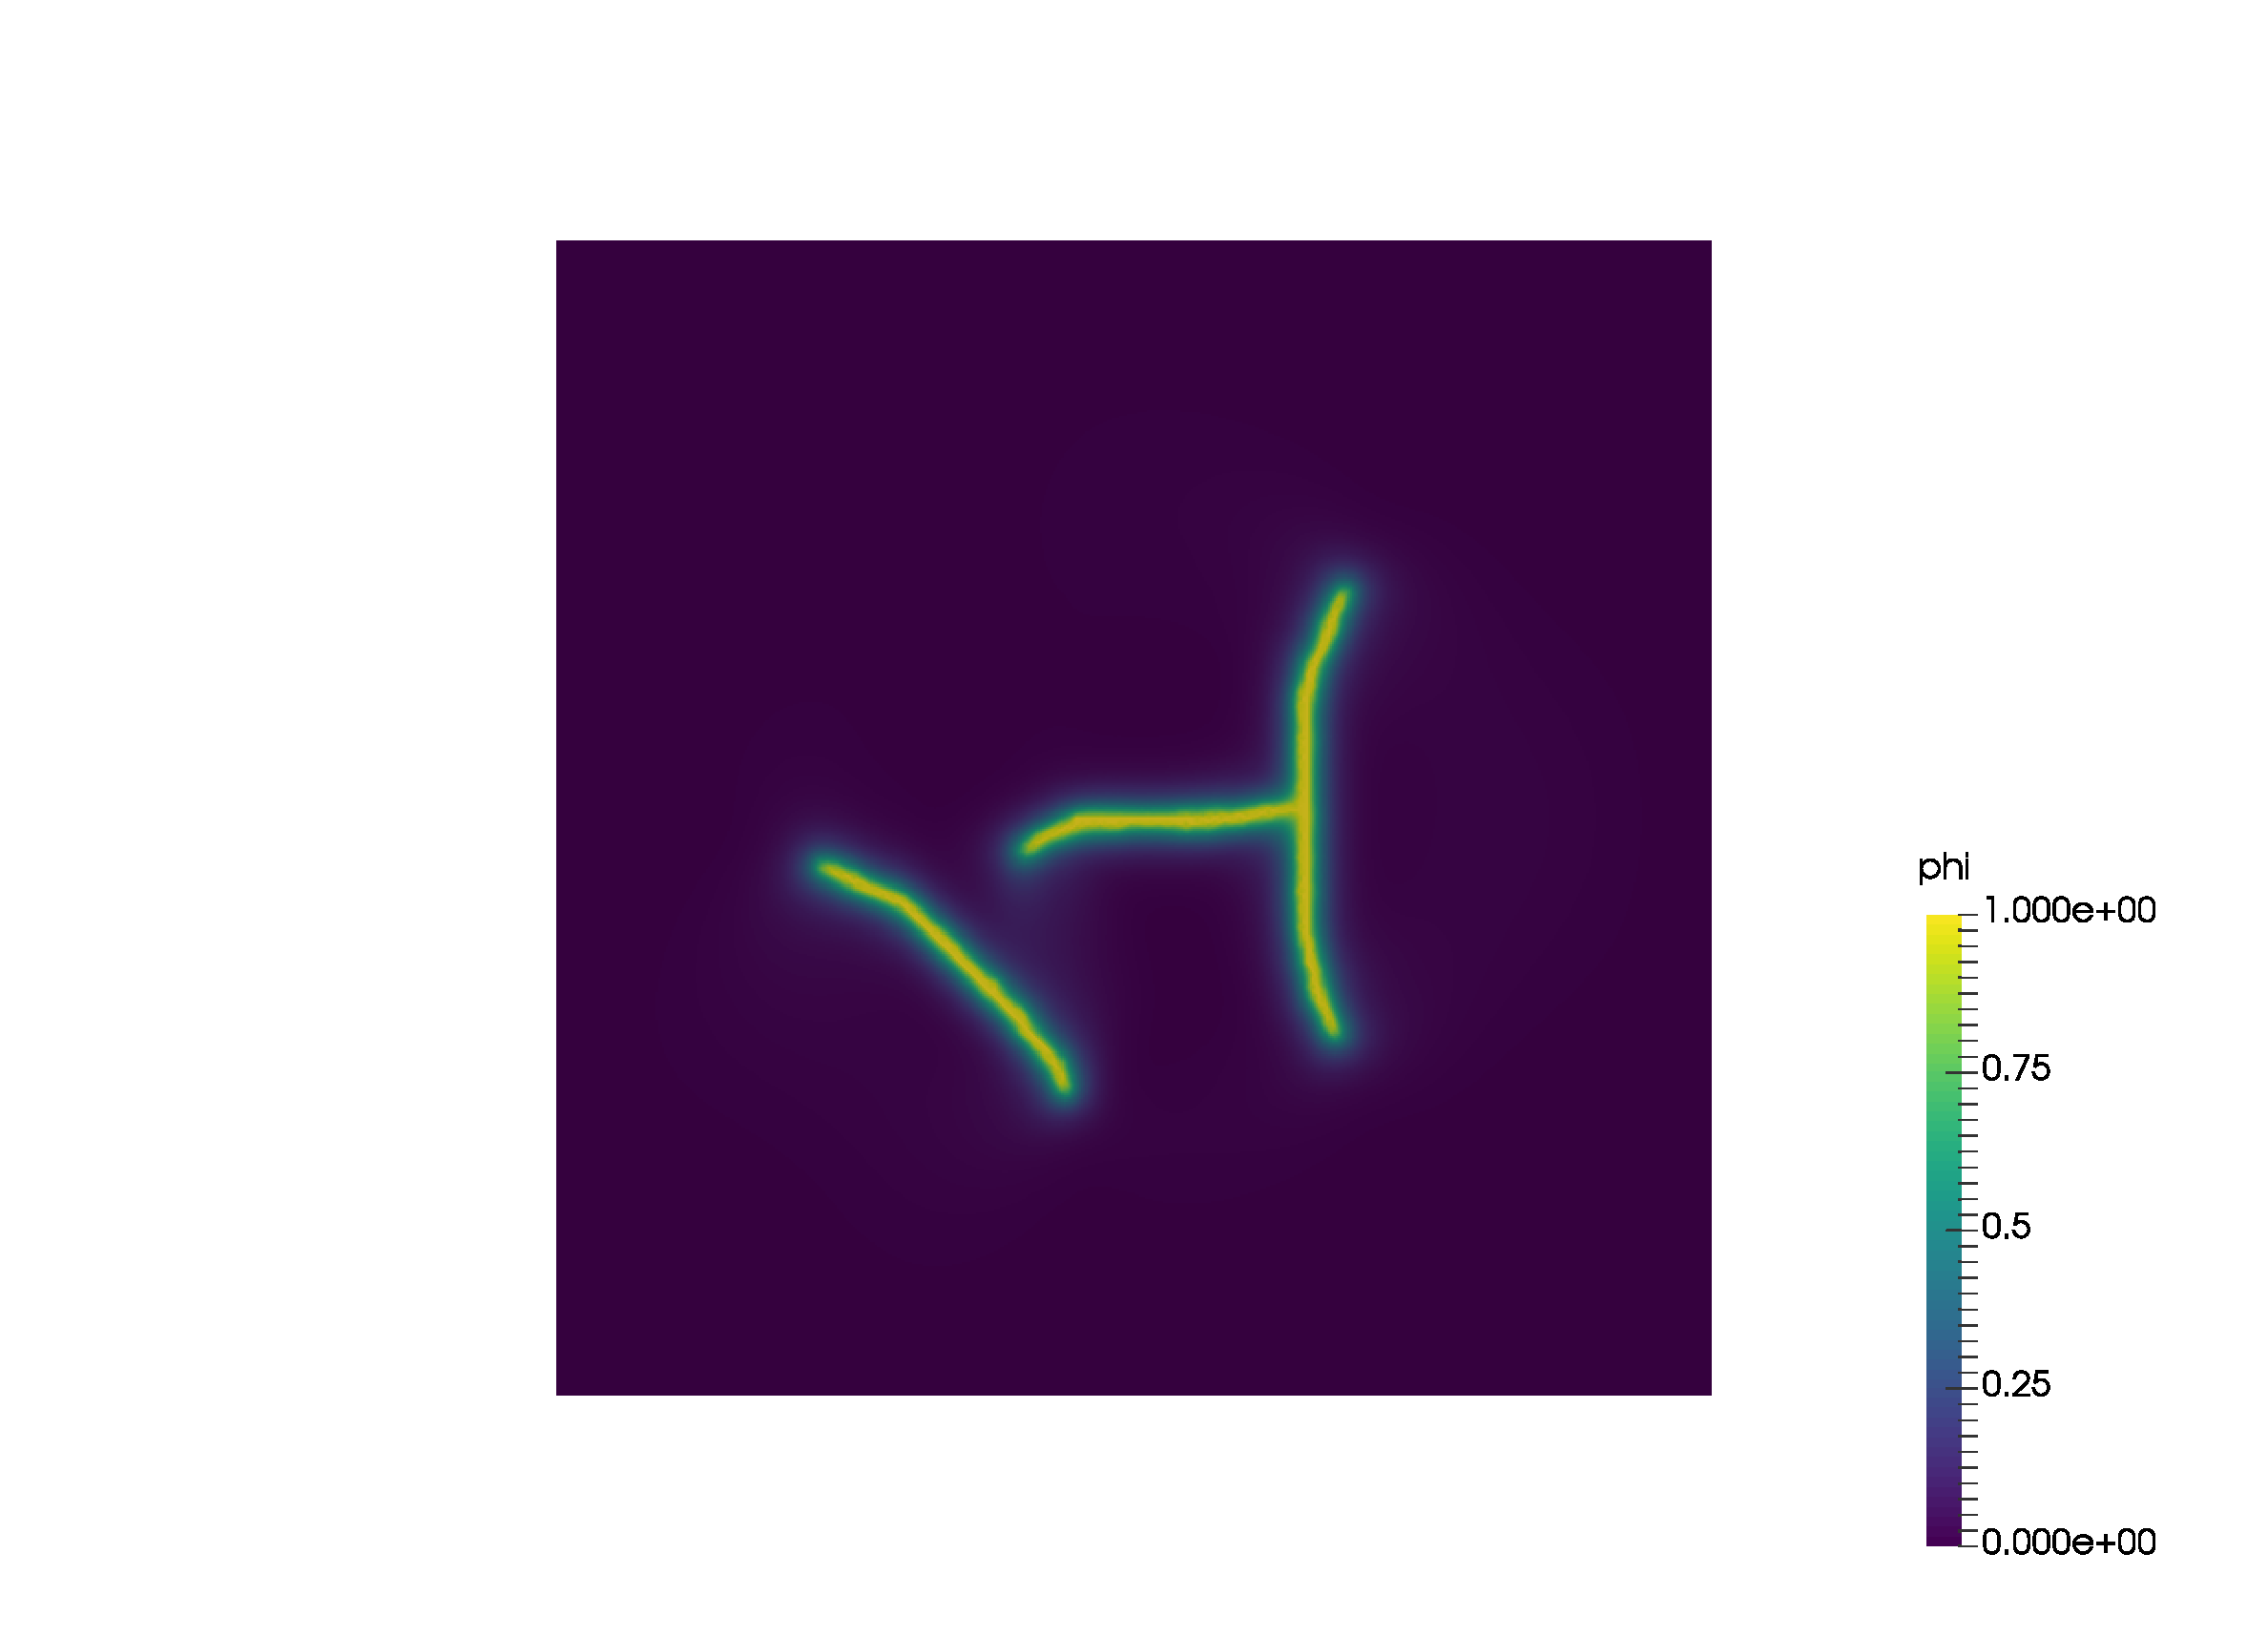
\includegraphics[width=5cm,trim=7cm 1cm 7cm 1cm, clip]{Images/TNF/tnf_d_0_024.pdf}};
    \end{tikzpicture}
    \caption{t = 0.024 [s]}
    \label{sec4:fig:tnf_d_0_024}
  \end{subfigure}
  \hspace{2.5mm}
  \begin{subfigure}[t]{0.275\textwidth}
  \centering
    \begin{tikzpicture}
    \node[inner sep=0pt] () at (0,0)
    {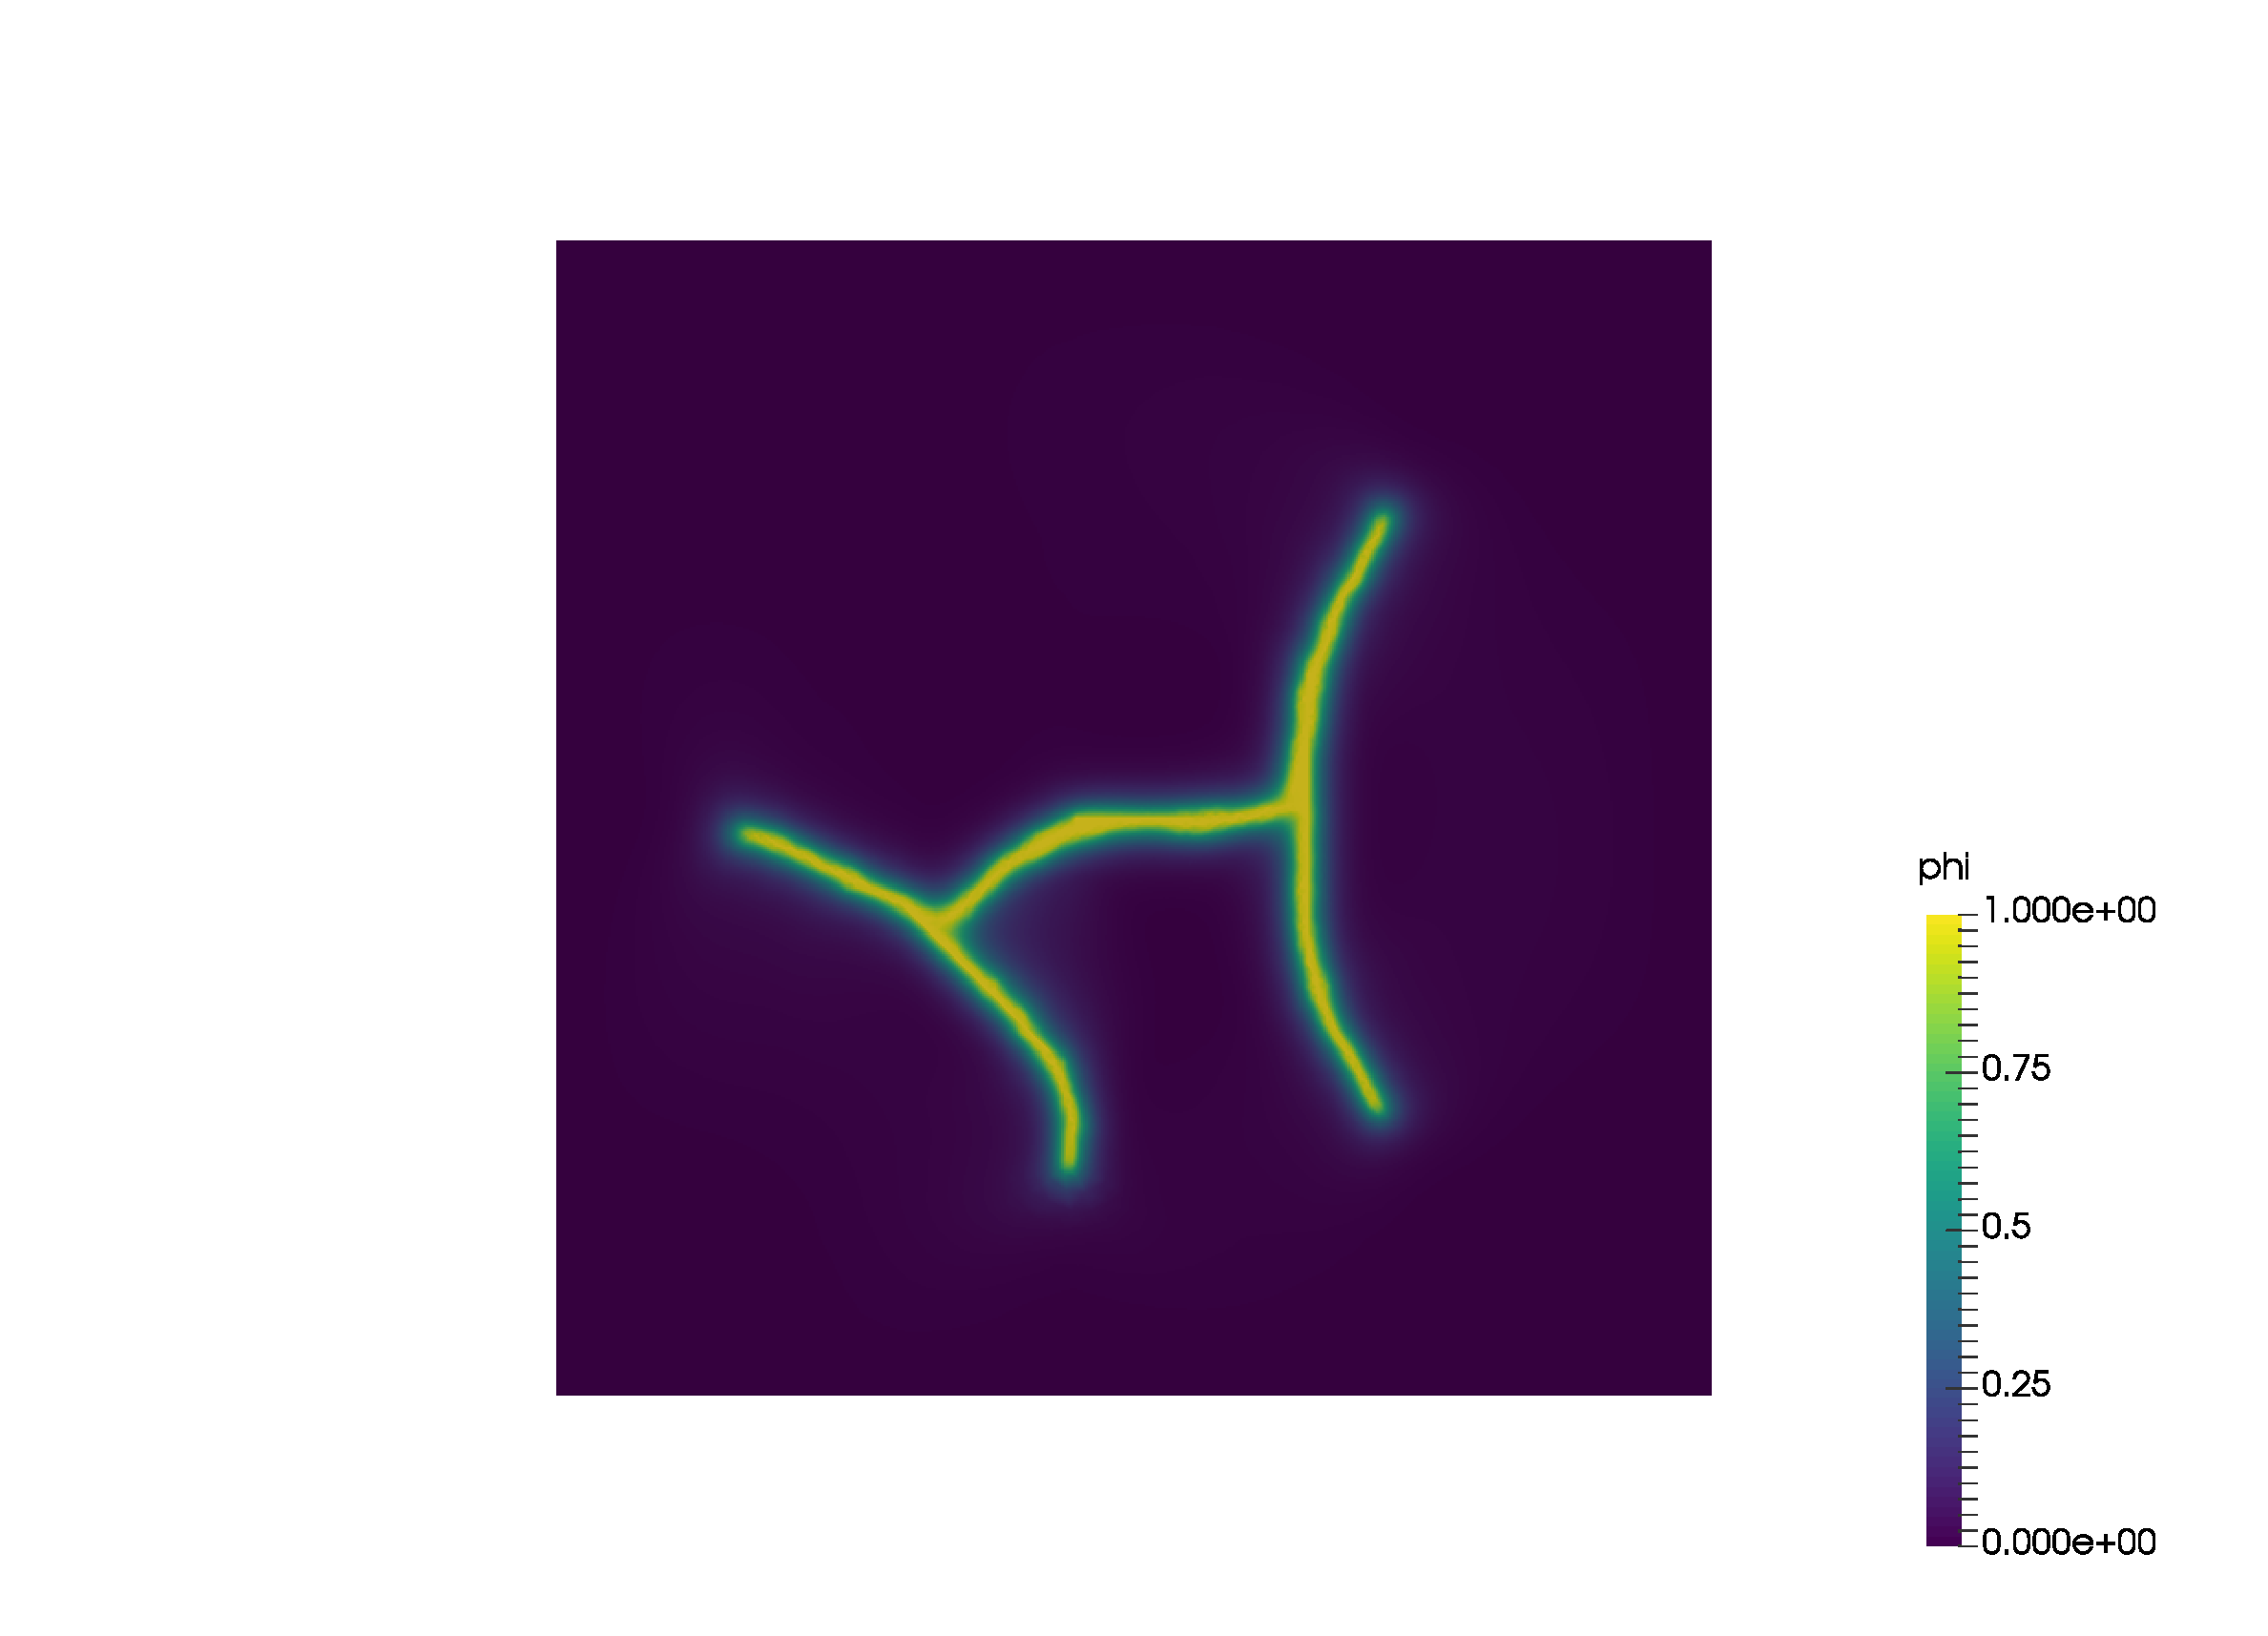
\includegraphics[width=5cm,trim=7cm 1cm 7cm 1cm, clip]{Images/TNF/tnf_d_0_048.pdf}};
    \end{tikzpicture}
    \caption{t = 0.048 [s]}
    \label{sec4:fig:tnf_d_0_048}
  \end{subfigure}
  \hspace{0.5mm}
  \begin{subfigure}[t]{0.05\textwidth}
  \setlength{\unitlength}{1pt}
    \begin{picture}(1,1)
    \put(-80.,-16){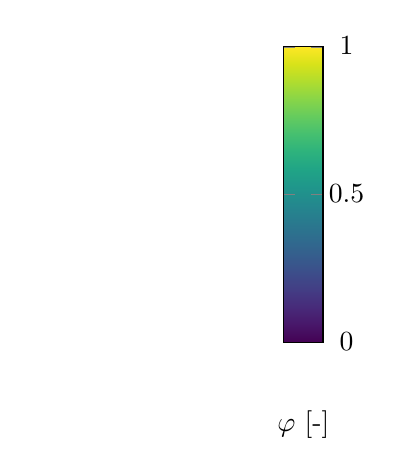
\begin{tikzpicture}[rotate=0]
    {\begin{axis}[
    hide axis,
    scale only axis,
    height=0pt,
    width=0pt,
    colormap/viridis,
    colorbar horizontal,
    point meta min=0,
    point meta max=1,
    colorbar style={
        width=3.75cm,
        rotate=90,
        at={(0.0,50.0)},anchor=south,   
        xtick={0,0.5,1.0},
        xticklabel style = {yshift=0.25cm},
        xticklabel style = {xshift=0.3cm}
    }]
    %\addplot [draw=none] coordinates {(1.5,0)};
    \end{axis}};
    \node[inner sep=0pt] () at (0,-1.05) {$\pf$ [-]};
    \end{tikzpicture}}
    \end{picture}
  \end{subfigure}
  \caption{Figures (a-c) present the distribution of the phase-field variable at the different times during the analysis of the Three Natural Fractures (TNF) specimen.}
  \label{sec4:fig:tnf_pf}
\end{figure}

\begin{figure}[!ht]
\centering
  \begin{subfigure}[t]{0.275\textwidth}
  \centering
    \begin{tikzpicture}
    \node[inner sep=0pt] () at (0,0)
    {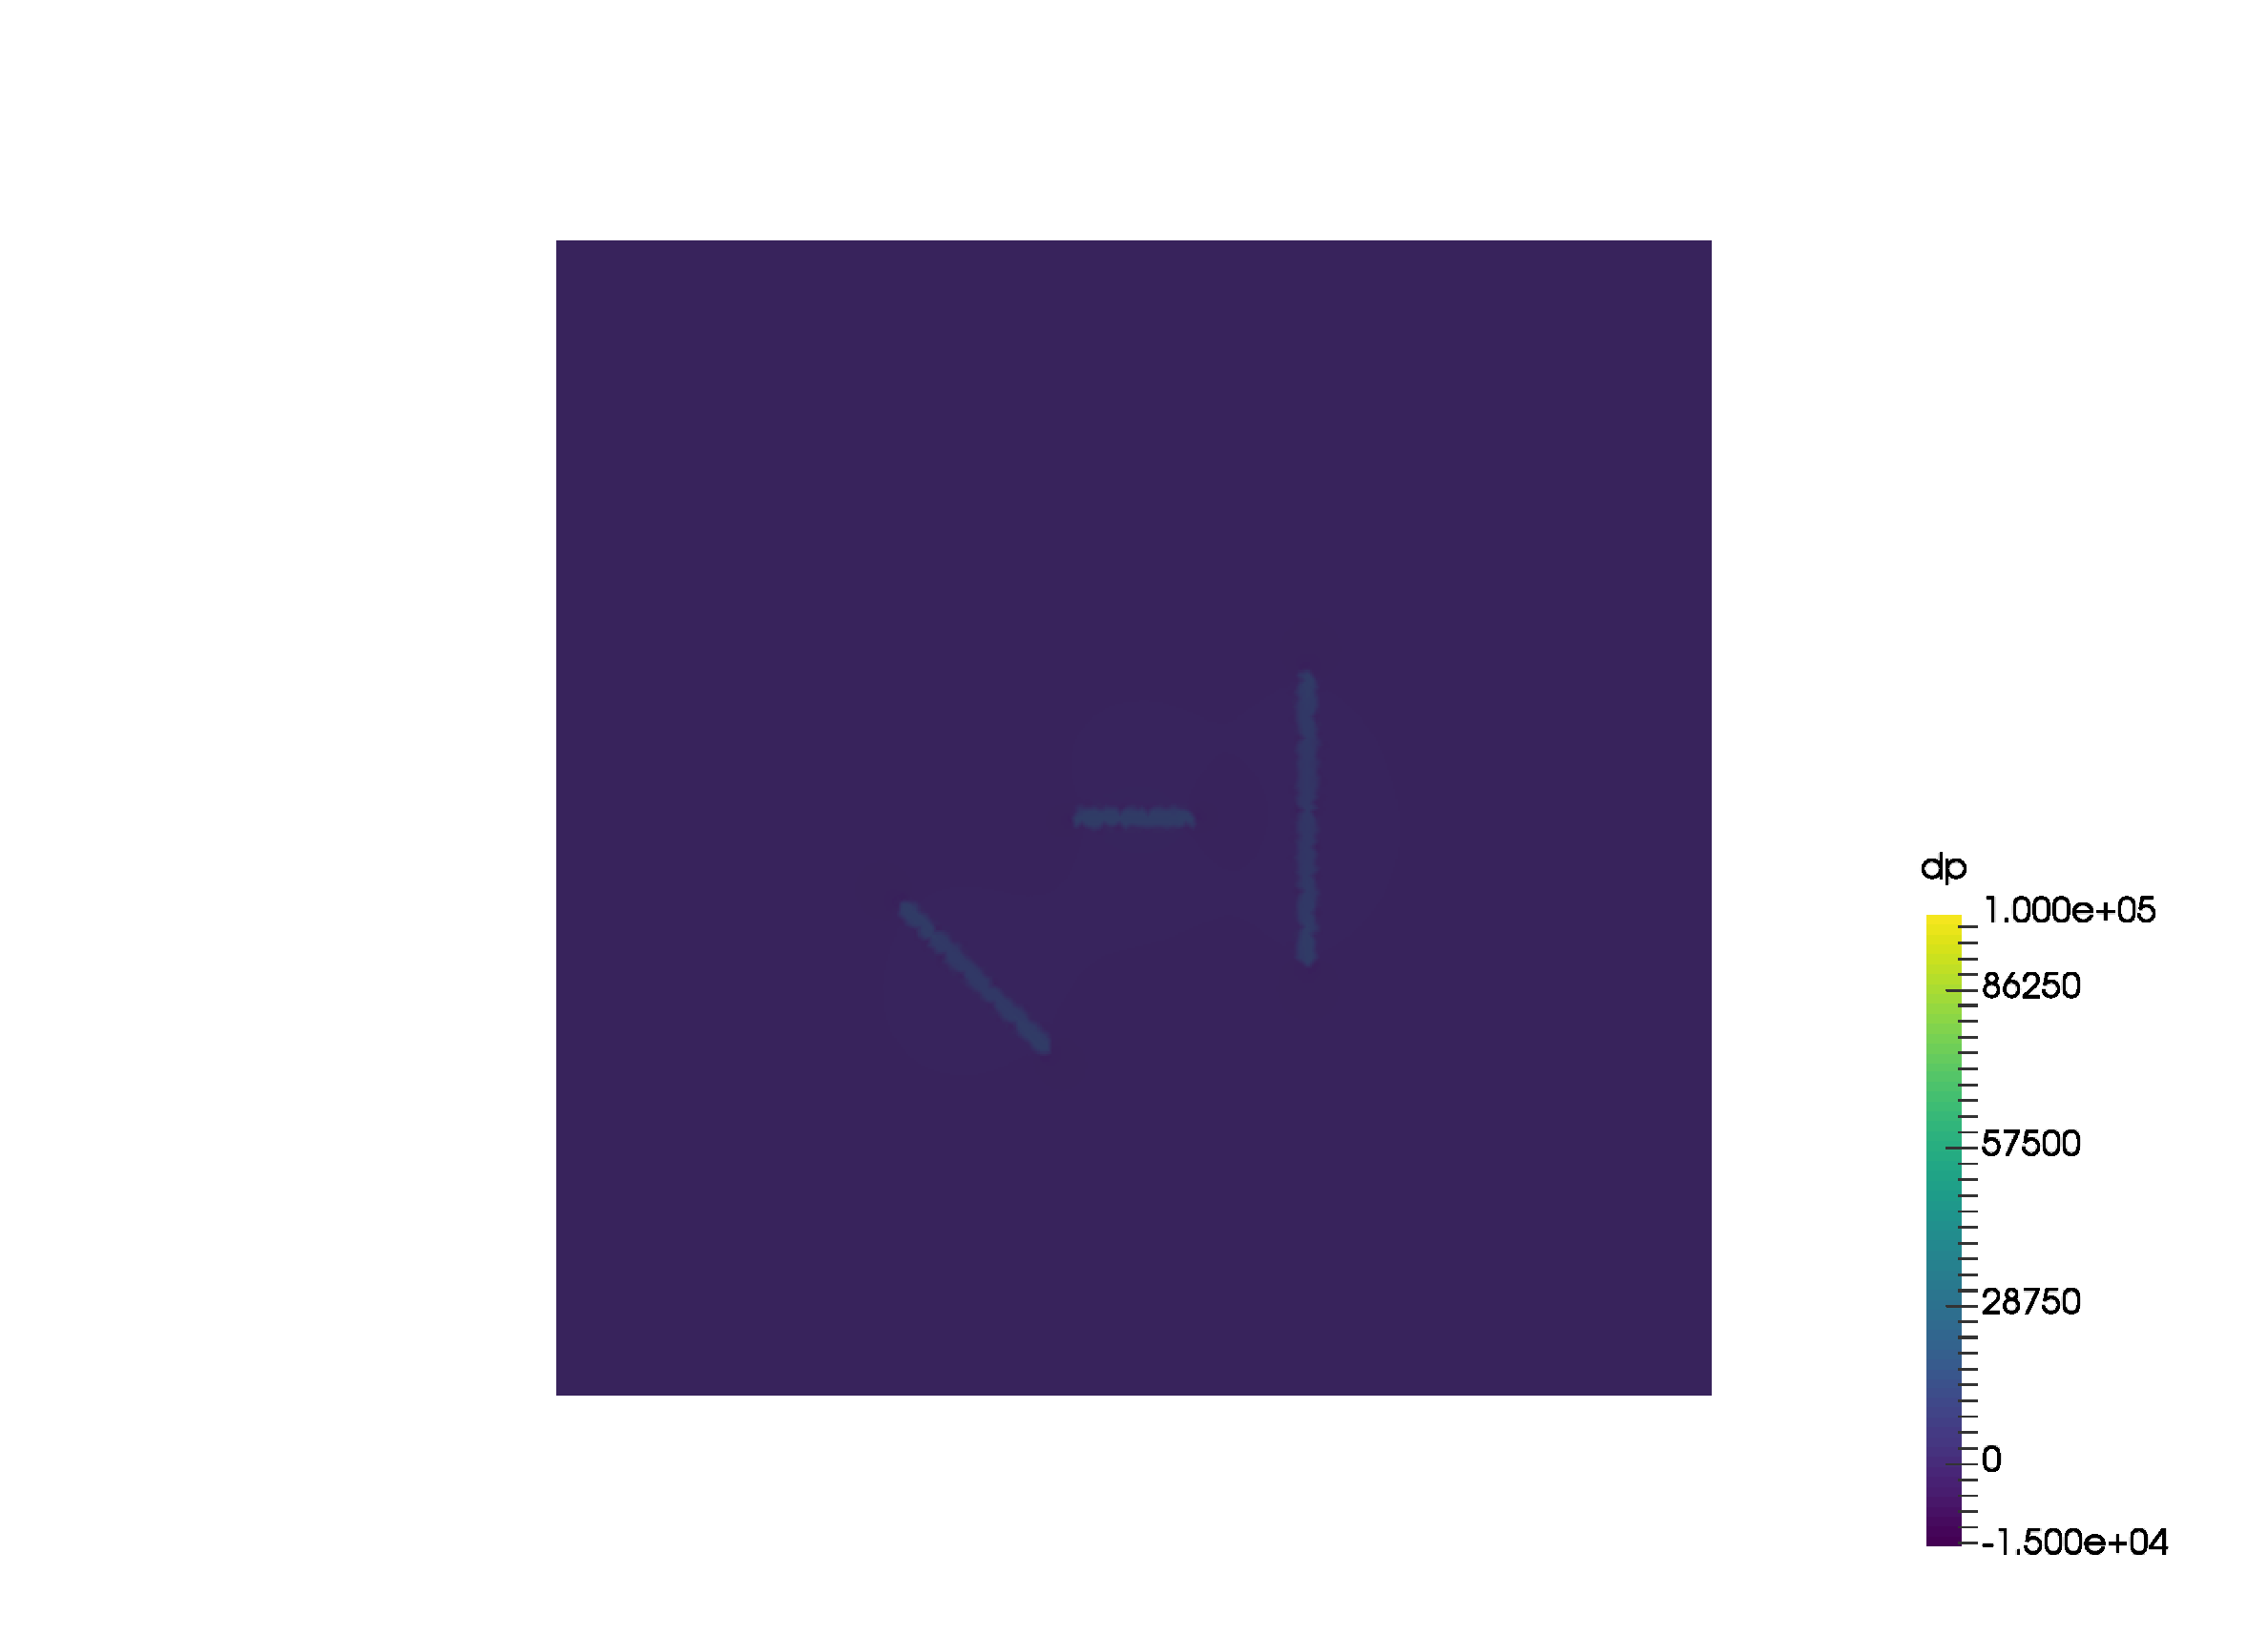
\includegraphics[width=5cm,trim=7cm 1cm 7cm 1cm, clip]{Images/TNF/tnf_p_0_0.pdf}};
    \end{tikzpicture}
    \caption{t = 0.001 [s]}
    \label{sec4:fig:tnf_p_0_0}
  \end{subfigure}
  \hspace{2.5mm}
  \begin{subfigure}[t]{0.275\textwidth}
  \centering
    \begin{tikzpicture}
    \node[inner sep=0pt] () at (0,0)
    {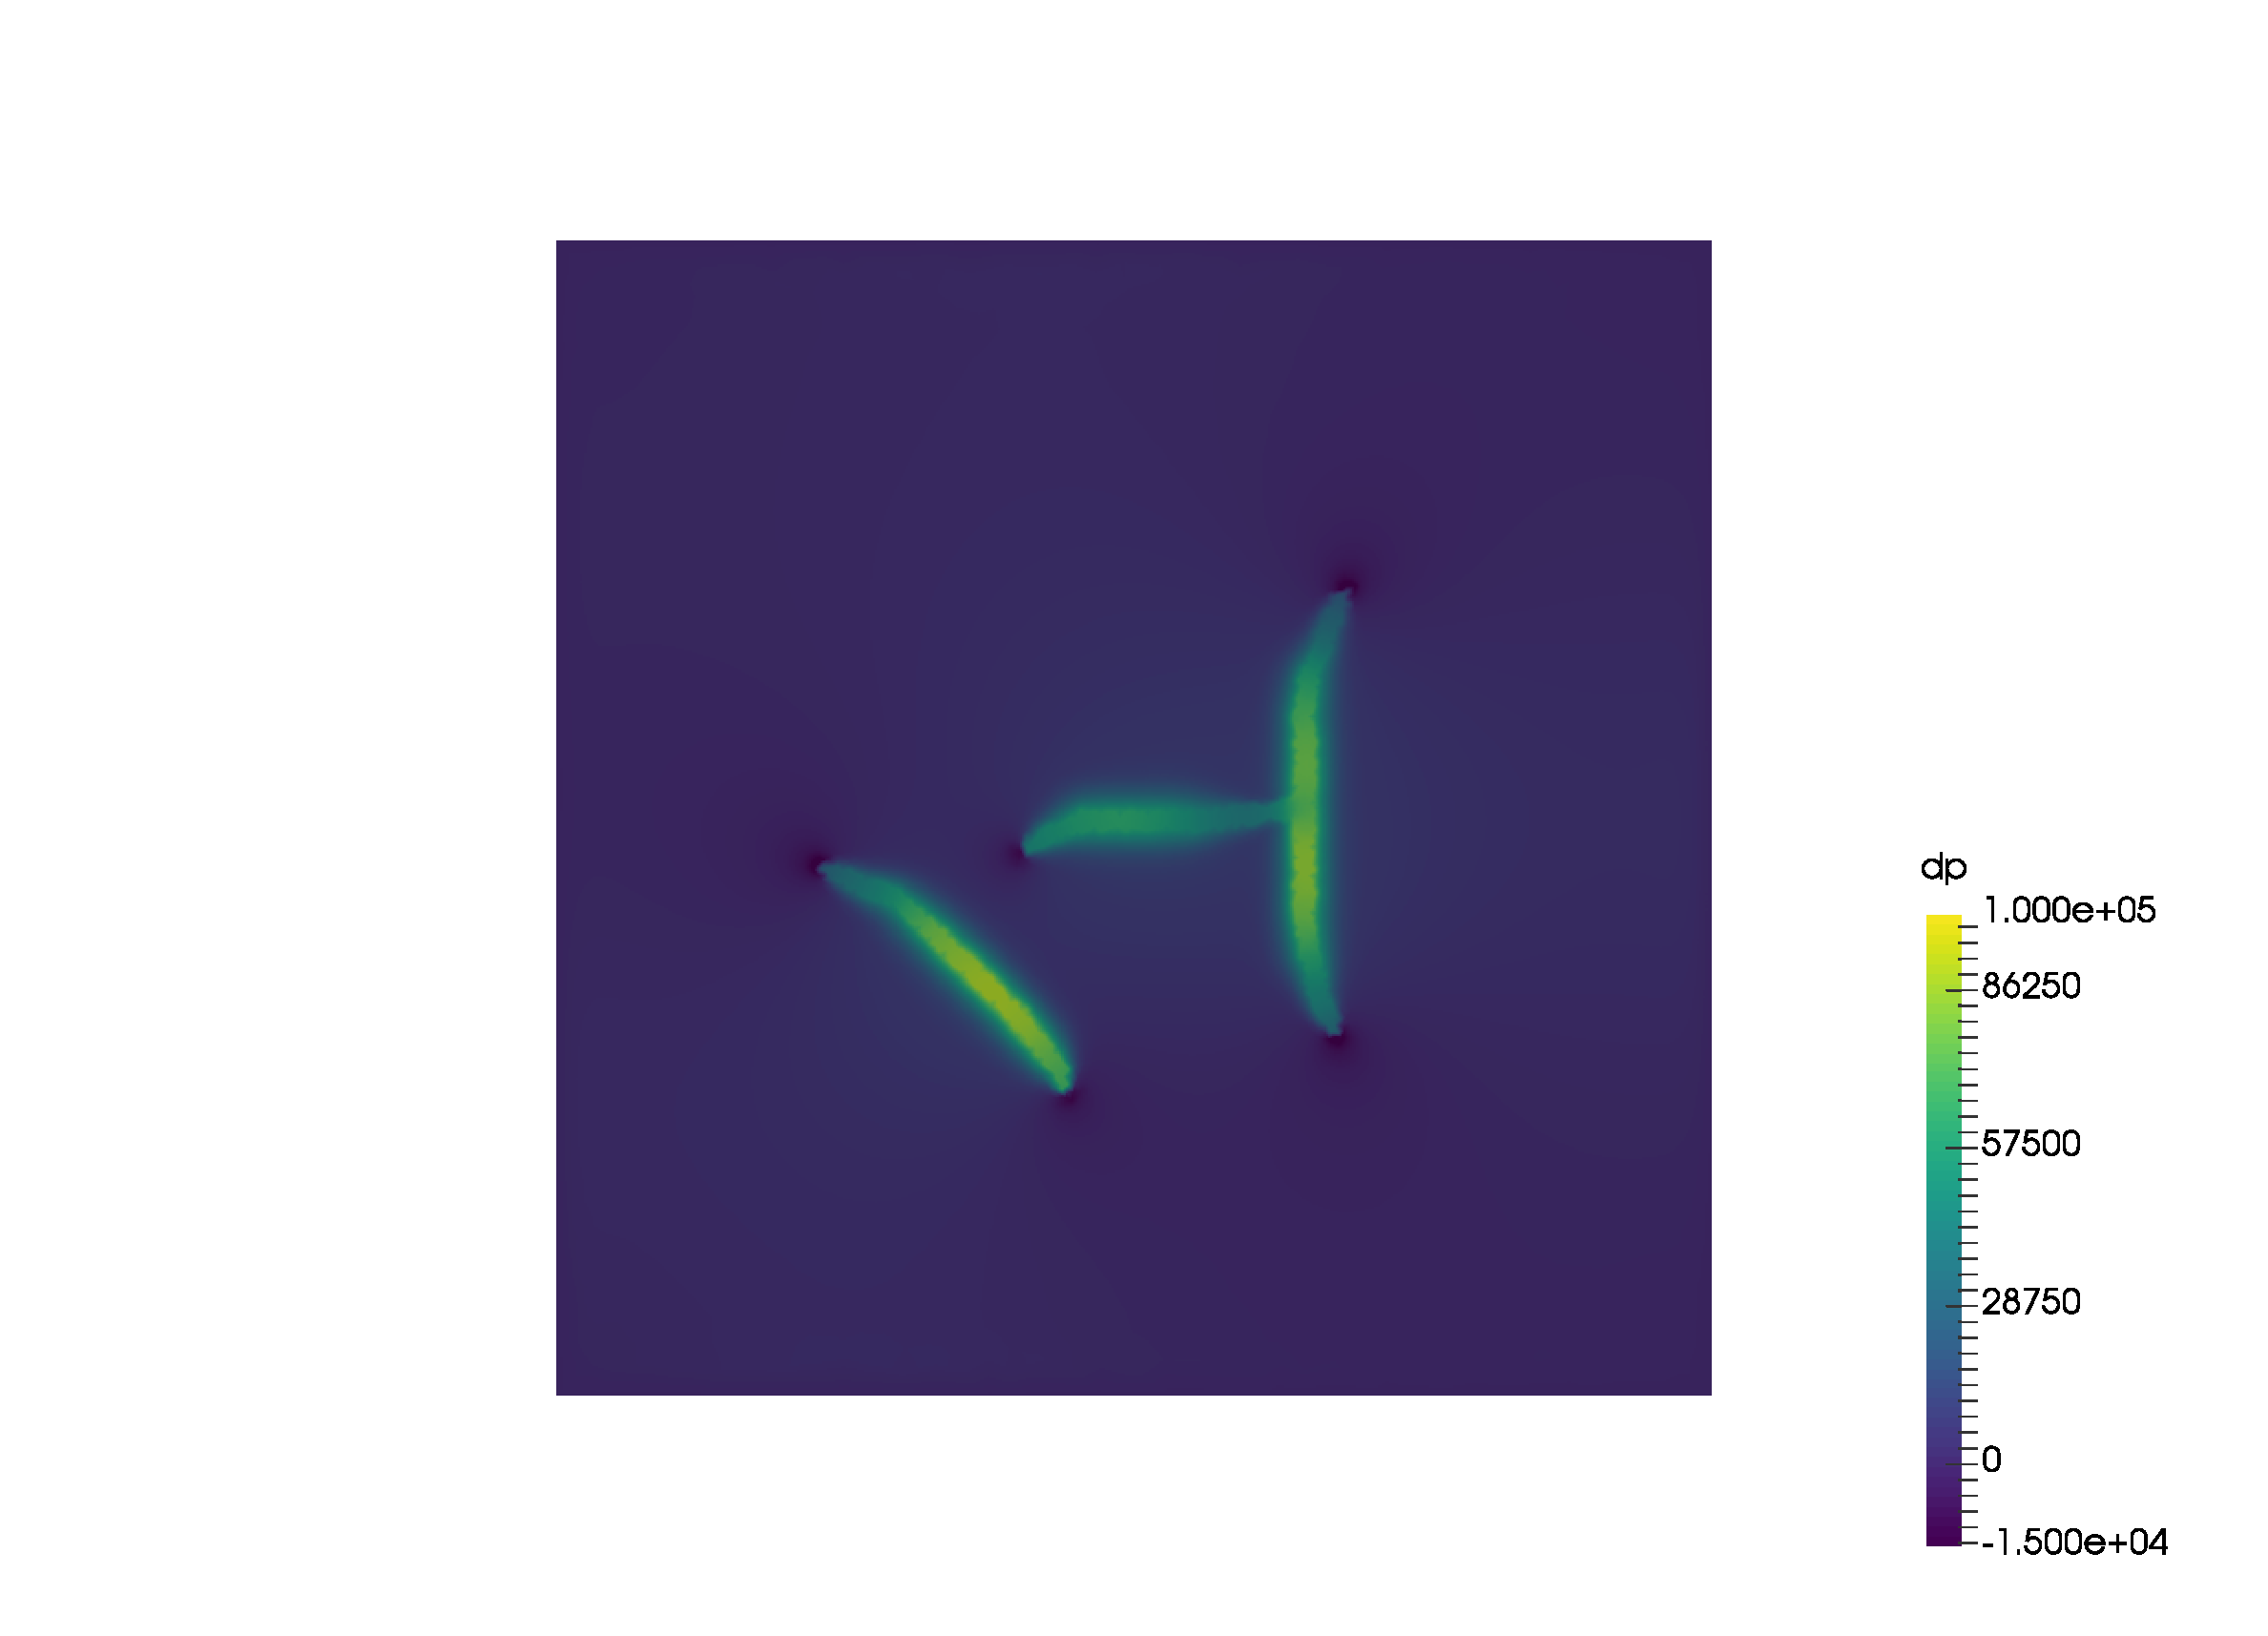
\includegraphics[width=5cm,trim=7cm 1cm 7cm 1cm, clip]{Images/TNF/tnf_p_0_024.pdf}};
    \end{tikzpicture}
    \caption{t = 0.024 [s]}
    \label{sec4:fig:tnf_p_0_024}
  \end{subfigure}
  \hspace{2.5mm}
  \begin{subfigure}[t]{0.275\textwidth}
  \centering
    \begin{tikzpicture}
    \node[inner sep=0pt] () at (0,0)
    {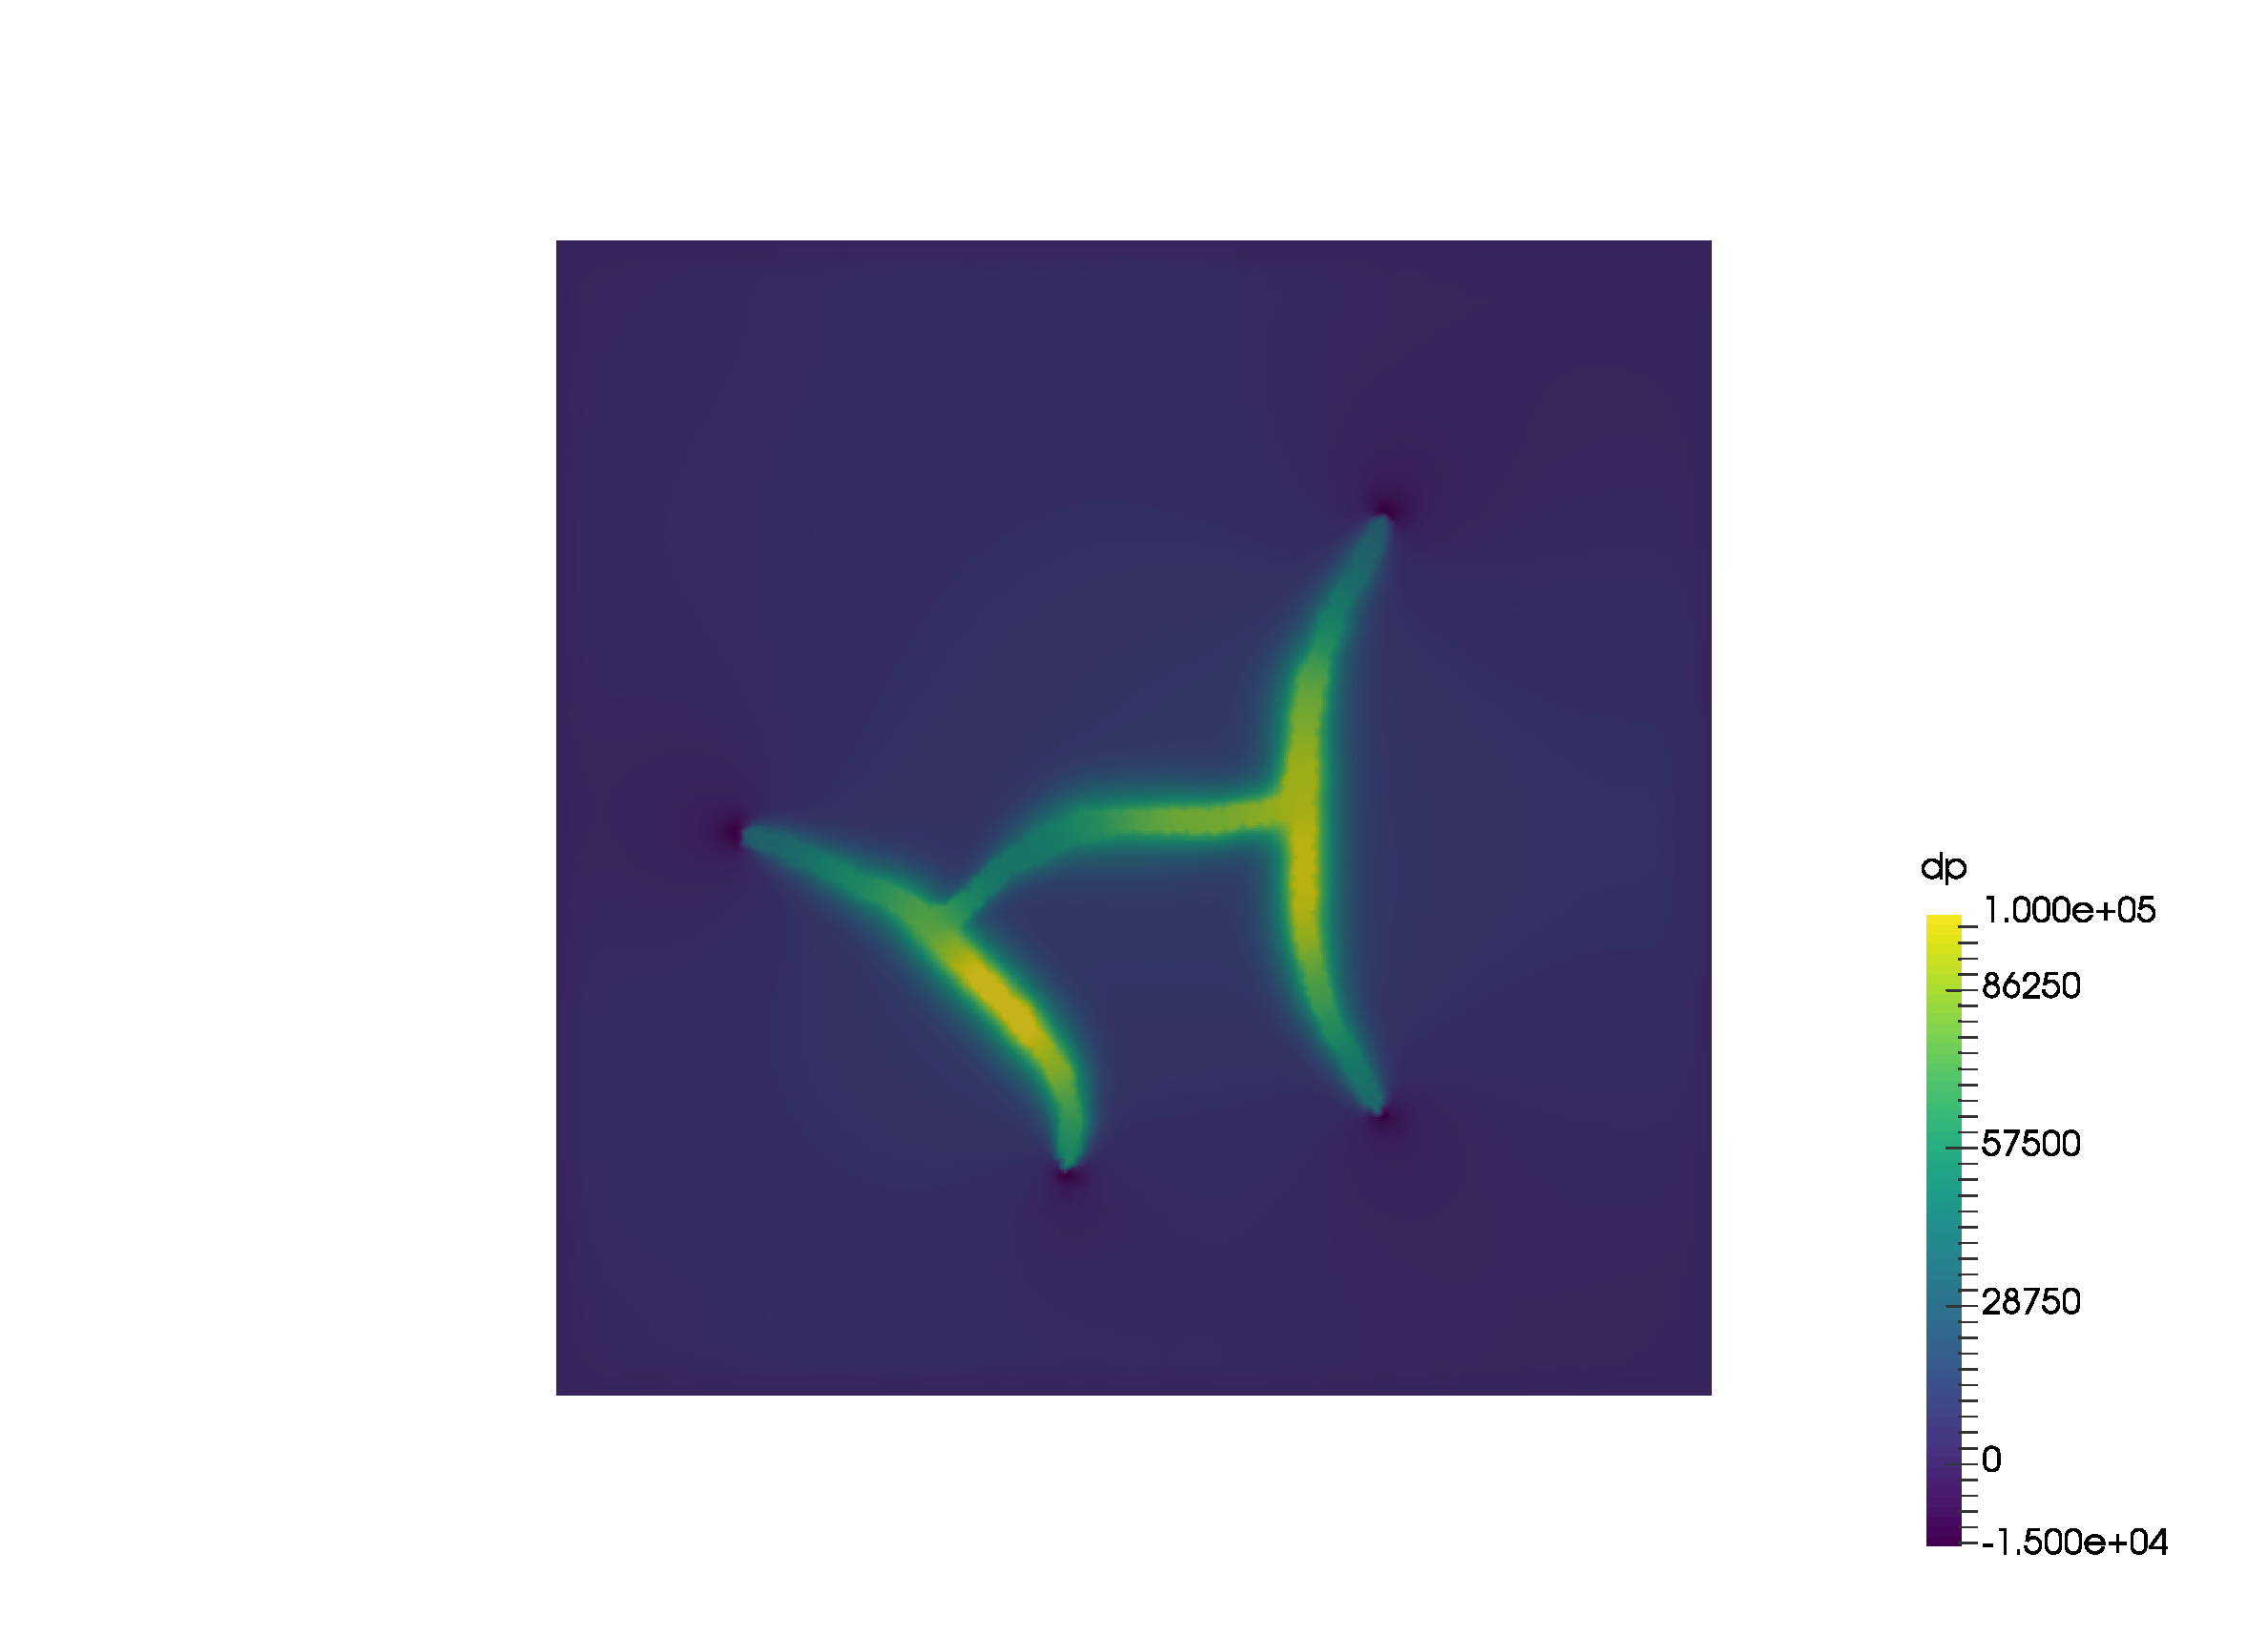
\includegraphics[width=5cm,trim=7cm 1cm 7cm 1cm, clip]{Images/TNF/tnf_p_0_048.pdf}};
    \end{tikzpicture}
    \caption{t = 0.048 [s]}
    \label{sec4:fig:tnf_p_0_048}
  \end{subfigure}
  \hspace{0.5mm}
  \begin{subfigure}[t]{0.05\textwidth}
  \setlength{\unitlength}{1pt}
    \begin{picture}(1,1)
    \put(-80.,-16){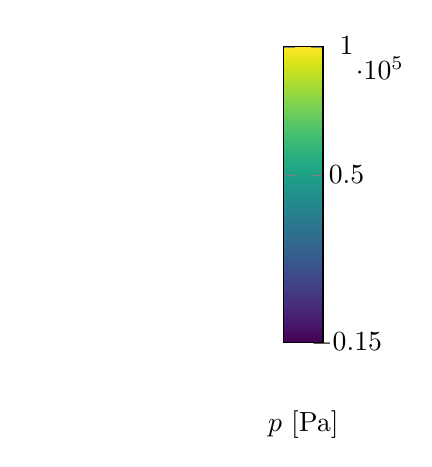
\begin{tikzpicture}[rotate=0]
    {\begin{axis}[
    hide axis,
    scale only axis,
    height=0pt,
    width=0pt,
    colormap/viridis,
    colorbar horizontal,
    point meta min=-15000,
    point meta max=100000,
    colorbar style={
        width=3.75cm,
        rotate=90,
        at={(0.0,50.0)},anchor=south,   
        xtick={-15000,50000,100000},
        xticklabel style = {yshift=0.25cm},
        xticklabel style = {xshift=0.3cm}
    }]
    %\addplot [draw=none] coordinates {(1.5,0)};
    \end{axis}};
    \node[inner sep=0pt] () at (0,-1.05) {$p$ [Pa]};
    \end{tikzpicture}}
    \end{picture}
  \end{subfigure}
  \caption{Figures (a-c) present the distribution of the fluid pressure at the different times during the analysis of the Three Natural Fractures (TNF) specimen.}
  \label{sec4:fig:tnf_pres}
\end{figure}

\color{black}

\section{Conclusions and Outlook}\label{sec5}

A novel phase-field fracture model is proposed in this manuscript, based on the micromorphic extension of the phase-field fracture energy functional. In this model, the phase-field variable is local, and a `new' micromorphic variable is introduced for regularization. In conjunction with the fracture irreversibility criterion, the phase-field evolution equation is a local variational inequality. This local equation is then solved pointwise (i.e., at integration points) in the computational domain. For brittle AT1 and AT2 fracture models, an explicit closed-form expression exist for the phase-field. However, for quasi-brittle fracture models, a nonlinear scalar equation needs to be solved iteratively. Furthermore, the local nature of the phase-field also provides the ease in implementing bounds, $\pf \in [0,1]$ using the trivial `\textit{min}' and `\textit{max}' operations. The micromorphic phase-field fracture model enforces fracture irreversibility and bounds on the phase-field with system-level precision without the need for any user-defined parameter, tracking of active/inactive sets, and without any loss of variational consistency.

The micromorphic phase-field fracture model converges towards the conventional phase-field fracture model for an appropriately chosen interaction parameter $\eta$. An appropriately chosen value of $\alpha$ results in $\pf \approx \mpf$, thereby establishing the equivalence of the energy functional of the two models. This convergent behaviour is demonstrated in this manuscript through numerical experiments on a single edge notched specimen loaded in tension with varying $\alpha$. For $\alpha \gtrsim 100 \gc / l$, $\pf \approx \mpf$ for an arbitrarily chosen section of the computational domain. In this case, both, the fracture topology as well as the load-displacement curve is similar to those obtained with conventional phase-field fracture models in the literature. For lower values of $\alpha$, the regularization is insufficient, and a local material behaviour is obtained. Additional numerical experiments were conducted, loading the aforementioned specimen in shear, and Winkler L-shaped panel and the concrete three-point bending tests for demonstrating quasi-brittle fracture phenomenon. For all experiments, the fracture topology as well as the load-displacement curve for $\alpha \gtrsim 100 \gc / l$ were in agreement with results from the literature. The micromorphic phase-field fracture model, is thus able to demonstrate both brittle and quasi-brittle fracture in linear elastic media.

Furthermore, the feasibility of extending the micromorphic phase-field fracture model towards multiphysics problems is demonstrated through hydraulic fracturing simulations. To this end, the energy functional developed for linear elastic media is extended towards porous media, with an additional fluid phase contribution. A fluid transport equation is added to the system of equations, wherein a dual permeability model is introduced. The dual permeability model is defined using a fracture dependent scaling function that iterates between the bulk and fracture intrinsic permeabilities. For a sufficiently high $\eta$, the phase-field $\pf \approx$ the micromorphic variable $\mpf$. This allows the construction of a fracture dependent scaling function using the micromorphic variable instead of the phase-field. This choice circumvents the additional derivatives of the scaling function w.r.t. the strain and the micromorphic variable. Numerical experiments in hydraulic fracture demonstrates the fracture merging capabilities of the micromorphic phase-field fracture model in a multiphysics hydraulic fracturing context.

Finally, the novel micromorphic phase-field fracture model opens a plethora of future research extensions, particularly, in other multi-physics applications, or composite laminates \cite{BUI2021107705}. Other studies may include the implementation of a dissipation-based arc-length method \cite{may2015numerical,BHARALI2022114927} or quasi-Newton methods \cite{KRISTENSEN2020102446,WU2020112704} for addressing the non-convexity of energy functional. 

\section{Software Implementation and Data Availability}

The numerical study in Section \ref{sec5} is carried out using a C++ software package \texttt{falcon}, inspired by \texttt{ofeFRAC} \cite{NGUYENTHANH2020102925}, and based on the Jem and Jive libraries from the Dynaflow Research Group, the Netherlands. The source code as well as the data set would be made available in Github repository of the corresponding author (\url{https://github.com/ritukeshbharali/falcon}).

\section*{Acknowledgements}

The financial support from the Swedish Research Council for Sustainable Development (FORMAS) under Grant 2018-01249 and the Swedish Research Council (VR) under Grant 2017-05192 is gratefully acknowledged. The first author would also like to thank Erik Jan Lingen at Dynaflow Research Group for support with the Jem and Jive libraries, and Vinh Phu Nguyen at Monash University for granting free access to \texttt{ofeFRAC} source files.


\printbibliography

\end{document}